\documentclass[12pt,a4paper]{article}

\usepackage[utf8]{inputenc}
\usepackage[english, russian]{babel}
\usepackage{indentfirst}
\usepackage{misccorr}
\usepackage{graphicx}
\usepackage{floatflt}
\usepackage{amsmath}
\usepackage{amsfonts}
\usepackage{color}
\usepackage{hyperref}
\usepackage[normalem]{ulem}
\usepackage{cancel}

\hypersetup{
	colorlinks=true, % make the links colored
	linkcolor=black, % color TOC links in blue
	urlcolor=blue, % color URLs in red
	linktoc=all % 'all' will create links for everything in the TOC
}

\author{Andrei Tkachuk}
\title{Конспет по высшей математике (3 семестр)}

\begin{document}
	\newtheorem{Def}{Определение}[section]
	\newtheorem{Th}{Теорема}[section]
	\newtheorem{Seq}{Следствие}[section] %потом было бы неплохо сделать так, чтобынумерация следствий была не по параграфам, а по теоремам в параграфе
	\newtheorem{Lem}{Лемма}[section]
	\newtheorem{Axiom}{Аксиома}[section]
	\newtheorem{Note}{Замечание}[section]
    \newtheorem{Example}{Пример}[section]

	 % Оформление докозательства
	\newenvironment{Proof} % имя окружения
	{\par\noindent{\bf Доказательство.}} % команды для \begin
	{\hfill$\scriptstyle\blacksquare$} % команды для \end
	
	%градиент
    \newcommand{\grad}[2]{\mathop{\mathrm{grad}} #1 |_{#2}}
	%специальная буква из \mathbb для множеств чисел
	\newcommand\bb[1]{\mathbb{#1}}
	%обозначение вектора
	\newcommand\Vectr[1]{\overrightarrow{#1}}
    % 'фи' равно красивой 'фи'
    \renewcommand{\phi}{\varphi}
    % Определение русской действительной части вместо \Re
    \renewcommand{\Re}{\mathop{\text{Re}}} 
    % Определение стандартного ряда
    \newcommand{\baserow}[1]{\sum\limits_{n = 1}^{+\infty}{#1}}
    
    
	\tableofcontents
    %File:         %No  %Status:
    \author{Andrei Tkachuk}
\part{Приложение функции нескольких переменных}
\section{Касательные к пространственным прямым и касательные к поверхностям}
		\begin{Def}[Касательная к пространственным кривым]
			Пусть $L$ --- гладкая пространственная кривая без особых точек или
			\begin{gather*}
				L : 
				\begin{cases}
					x = x(t) \\
					y = y(t) \\
					z = z(t) \\
				\end{cases} t \in U(t_0) \\ 
				x(t), y(t), z(t) \in C'(U(t_0)) \quad (x'_t, y'_t, z'_t) \neq (0, 0, 0) 
			\end{gather*}
		\end{Def}   
        Геометрически выглядит следующим образом
        \begin{figure}[bh]
            \noindent\centering{
                \includegraphics[width=65mm]{pictures/1_1_1.png}
                \caption{}
            }
        \end{figure}\\
        Обозначим
        \[
            	M_0(x_0, y_0, z_0) \quad \text{при}\; t = t_0 \qquad \Delta t \neq 0, \; t = t_0 + \Delta t, \; \Delta t \in  U(t_0)
        \]
        Тогда уравнение касательной
		\begin{equation*}
            MM_0 :\: \frac{x - x_0}{x (t_0 + \Delta t) - x_0} = \frac{y - y_0}{y (t_0 + \Delta t) - y_0} = \frac{z - z_0}{z (t_0 + \Delta t) - z_0}
		\end{equation*}
		Равенство выше является каноническим. Если разделить элементы на $\Delta t$ и рассмотреть $\Delta t \rightarrow 0$ то получим следующее
		\begin{gather*}
			l_0 \: : \frac{x - x_0}{x'_0} = \frac{y - y_0}{y'_0} = \frac{z - z_0}{z'_0}
        \end{gather*}
        Так как 
        \begin{equation*}
            \frac{x(t_0 - \Delta t) - x(t_0)}{\Delta t} \to x'_t(t_0) = x'_0 \qquad \Delta t \to 0 \\
		\end{equation*}
		$l_0$ --- касательная к кривой $L$ в точке $M_0$ \\
		$l_0$ --- кривая линия в пространстве ${x'_0} \cdot {y'_0} \cdot {z'_0} \neq 0$
		
		
		\begin{Def}~\\
			Пусть $S : F(x, y, z) = 0$ --- поверхность в пространстве.\\
            $F(x, y, z)$ --- непрерывная функ. в окрестности точки $M_0(x_0, y_0, z_0) \in S$\\
			Плоскость $\pi : Ax + By + Cz + D = 0$, где $A^2 + B^2 + C^2 \neq 0$ называется касательная плоскость к $S$ в точке $M_0$ если
			\begin{enumerate}
				\item $M_0 \in \pi$ 
				\item Любая кривая линия $L \subset S, M_0 \in L$ гладкой кривой с направляющим вектором касательной $\vec{\tau} \neq \vec{0}$ выполняется условие 
                \[
                    \vec{n} \perp \vec{\tau}, \vec{n} = {A, B, C} \quad \Leftrightarrow \quad (\vec{n}, \vec{\tau}) = 0
                \]
			\end{enumerate}
			
         	\begin{figure}[bh]
            \noindent\centering{
                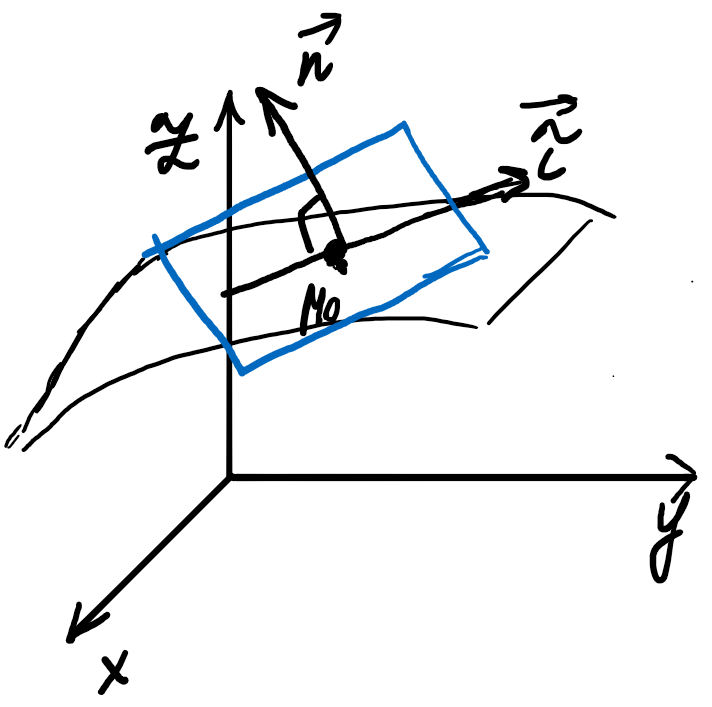
\includegraphics[width=65mm]{pictures/1_1_2.png}
                \caption{}
            }
            \end{figure}
						
		\end{Def}
	
		\begin{Th}[О существовании касательной плоскости] Пусть
            \[
                F(x, y, z) \in C^1(U(M_0)), \quad {F'_x}^2(M_0) + {F'_y}^2(M_0) + {F'_z}^2(M_0) \neq 0
            \]
			Тогда для поверхности $S : F(x, y, z) = 0, \; M_0(x_0, y_0, z_0) \in S$ существует касательная плоскость 
            \[
                \pi : F'_x(M_0)\,(X-x_0) + F'_y(M_0)\,(Y-y_0) s+ F'_z(M_0)\,(Z-z_0) = 0
            \]
		\end{Th}
		\begin{Proof}
			\begin{align*}
			&L:\begin{cases}
					x = x(t)\\
					y = y(t)\\
					z = z(t)\\	
			   \end{cases} \; t \in U(t_0) \quad x(t),\, y(t),\, z(t) \in C^1(U(t_0))\\
			&x_0 = x(t_0), \; y_0 = y(t_0), \; z_0 = z(t_0), \quad M_0(x_0,\, y_0,\, z_0) \in L\\
			&\vec{\tau} = {x'_t(t_0),\, y'_t(t_0),\, z'_t(t_0)}\\
			&\vec{n} = {F'_x(M_0),\, F'_y(M_0),\, F'_z(M_0)}
			\end{align*}
            Докажем, что скалярное произведение равно нулю
            \begin{align*}
			&L \subset S \Rightarrow \forall t \in U(t_0) \; F(x(t),\, y(t),\, z(t)) = 0\\
			&\text{Из дифференцируемости сложной функции получаем}\\
			&(F(x(t),\, y(t),\, z(t)))'_t = F'_x\, x'_t + F'_y\, y'_t + F'_z\, z'_t\\ &\text{при} \; t = t_0\\
			&F'_x(M_0)\,x'_t(t_0) + F'_y(M_0)\,y'_t(t_0) + F'_z(M_0)\,z'_t(t_0) = 0 \; \Rightarrow \; (\vec{n}, \vec{\tau}) = 0\\
			&\Rightarrow \; \pi : F'_x(M_0)\,(X-x_0) + F'_y(M_0)\,(Y-y_0) + F'_z(M_0)\,(Z-z_0) = 0
			\end{align*}
		\end{Proof}
		
		\begin{Def}[Градиент] Градиент функции $F$ в точке $M_0$ обозначается так
        \[ 
            \{F'_x(M_0);\; F'_y(M_0);\; F'_z(M_0)\} = \grad{F}{M_0}
        \]  
		\end{Def}
	
		\begin{Th}(Существование касательной плоскости к явно заданной поверхности).\\
            Рассматривается случай явно заданной поверхности\\
			Пусть $f(x, y) \in C^1(U(N_0)), \, N_0(x_0,\, y_0)$.\\
			Тогда для явно заданной поверхности $S : z = f(x, y)$ существует касательная плоскость в точке $M_0(x_0,\, y_0,\, z_0), \, \text{где } z_0 = f(N_0)$ вида 
			\[
                \pi: Z-z_0 = f'_x(N_0)\,(X-x_0) + f'_y(N_0)\,(Y-y_0)
            \]
		\end{Th}
		\begin{Proof}
			\begin{align*}
				&S: f(x, y) - z = 0, \, F = f(x, y) - z\\
				&F'_x = (f(x, y) - z)'_x = f'_x(N) \\ 
				&\text{Аналогично для других производных}\\
				&F'_y = f'_x(N); \; F'_z = -1;\\
				&\text{Т.к. мы задали явную функцию $F$, то по теореме 1 получаем}\\
				&\pi : f'_x(N_0)(X-x_0) + f'_y(N_0)(Y-y_0) + f'_z(N_0)(Z-z_0) = 0 \\
				&\pi : f'_x(N_0)(X-x_0) + f'_y(N_0)(Y-y_0) - (Z-z_0) = 0 ,\, \text{примечание } z_0 = f(x_0, y_0)\\
				&\pi : Z = f'(x_0, y_0) + f'_x(N_0)(X-x_0) + f'_y(N_0)(Y-y_0)
			\end{align*}
		\end{Proof}
		
		\begin{Def}[Нормаль к поверхности]
			Пусть $S : F(x,y,z) = 0, \; (x, y, z) \in U(M_0)$ гладкая поврхность. $M_0(x_0, y_0, z_0) \in S$.\\
			Тогда нормаль $\vec{n}$ к поверхности $S$ в точке $M_0$ называется прямая линия $n,\, M_0 \in n,\, n\perp\pi$, где $\pi$ --- касательная плоскость
		\end{Def}
		
		\begin{Note}
			Если в условии определения 4 $ \grad{F}{M_0} \neq \Vectr{0}$, то каноническое уравнение $n$
			\[
				n : \frac{x - x_0}{F'_x(M_0)} = \frac{y - y_0}{F'_y(M_0)} = \frac{z - z_0}{F'_z(M_0)}
			\] 
		\end{Note}
		  %1   %OK  R
    \author{Andrei Tkachuk}

\section{Экстремум функции нескольких переменных}

    \begin{Def}[Экстремума ФНП]
		Пусть функция $u = f(M) = f(x_1, \dots, x_n)$ --- является функцией n - переменных определённых в некоторой окрестности $U(M_0)$ и $M_0(x^0_1, \dots, x^0_n)$.\\
		Тогда
		\begin{enumerate}
			\item $M_0$ --- точкой (локального) минимума функции $f(M)$, если \\ 
            $\exists \delta > 0, \, \forall M \in U_\delta(M_0), \, f(M) \geqslant f(M_0)$
			
            \item $M_0$ --- точкой (локального) максимума функции $f(M)$, если \\ 
            $\exists \delta > 0, \, \forall M \in U_\delta(M_0), \, f(M) \leqslant f(M_0)$
            
        	\item $M_0$ --- точкой (локального) экстремума $f(M)$, если \\
             $M_0 = \min f(M)$ или $M_0 = \max f(M)$
		\end{enumerate}
	\end{Def}
	\begin{Def}[Строгий экстремум функции нескольких переменных]
		Пусть функция $u = f(M) = f(x_1, \dots, x_n)$ --- является функцией n - переменных определённых в некоторой окрестности $U(M_0)$ и $M_0(x^0_1, \dots, x^0_n)$\\
		Тогда
		\begin{enumerate}
			\item $M_0$ --- точкой строгого минимума функции $f(M)$, если\\
            $\exists \delta > 0, \, \forall M \in \mathring{U}(M_0), \, f(M) > f(M_0)$
            
			\item $M_0$ --- точкой строгого максимума функции $f(M)$, если\\
            $\exists \delta > 0, \, \forall M \in \mathring{U}(M_0), \, f(M) < f(M_0)$
			
            \item $M_0$ --- точкой строгого экстремума функции $f(M)$, если соблюдается пункт 1 или 2
		\end{enumerate}	
	\end{Def}

	\begin{Th}[Необходимое условие локального экстремума]
		Пусть существует функция 
        \begin{align*}
            &u = f(M) = f(x_1, \dots, x_n), \, M \in U_0(M_0)\\
            &\text{где }  M_0(x^0_1, \dots, x^0_n) \, \text{и } \exists f'_{x_1}, \dots, f'_{x_n}
        \end{align*}
		Тогда если $M_0$ --- точка локального экстремума, то 
        \[
            f'_{x_1}(M_0) = 0, \dots, f'_{x_n}(M_0) = 0 \Leftrightarrow df(M_0) = 0
        \]
	\end{Th}
	\begin{Proof}
		Пусть $M_0$ --- минимум f(M), т.е. 
        \[
            \exists \delta > 0, \, \forall M \in U_\delta(M_0), \, f(M) \geqslant f(M_0)
        \]
		Рассмотрим частную производную от первого аргумента через предел. Для этого возьмём точку $M(x_1, x^0_2, \dots, x^0_n)$ в окрестности точки $M_0$, тогда получаем\\
		\[
            f'_{x_1}(M_0) = \lim_{x_1 \to x^0_1}(\frac{f(x_1, x^0_2, \dots, x^0_n) - f(x^0_1, \dots, x^0_n)}{x_1 - x^0_1})
        \]
		Так как $M_0$ ---  минимум $f(M)$, то 
        \[
            f(M) - f(M_0) \geqslant 0
        \]
		Осталось рассмотреть два случая для знаменателя
		\begin{enumerate}
			\item если $x_1 > x^0_1$, то $f'_{x_1} \geqslant 0$
			\item если $x_1 < x^0_1$, то $f'_{x_1} \leqslant 0$
		\end{enumerate}
		Из всего этого следует, что 
        \[
            f'_{x_1}(M_0) = 0
        \] 
		Аналогично доказываются случаи для других производных
	\end{Proof}

	% Пример !!!
	%
	%
	%

	\begin{Lem}[О сохранении знака непрерывной функции]
		Пусть 
        \[
            u = \phi (M) = \phi (x_1, \dots, x_n) \in C(U(M_0))
        \]
        и
		\begin{enumerate}
			\item $\phi (M_0) > 0 \Rightarrow \exists \delta > 0 \; \forall M \in U_\delta (M_0) \; \phi (M) > 0$
			
            \item $\phi (M_0) < 0 \Rightarrow \exists \delta > 0 \; \forall M \in U_\delta (M_0) \; \phi (M) < 0$
		\end{enumerate}
	\end{Lem}

	\begin{Proof}
		\begin{enumerate}
			\item Логика доказательства аналогична первому семестру
                \begin{align*}
    				&\varphi (M_0) > 0 \\ 
    				&\varepsilon = \frac{\phi (M_0)}{2} > 0 \; \exists \delta > 0 \; \forall M \in U_\delta(M_0) \; | \varphi (M) - \varphi (M_0) | < \varepsilon \\
                    &\text{Расскроем знак модудя}\\
    				&\varphi (M_0) - \frac{\varphi (M_0)}{2} < \varphi (M) < \varphi (M_0) + \frac{\varphi(M_0)}{2}\\
    				&\Rightarrow \forall M \in U_\delta(M_0) \; \varphi(M) > \frac{\varphi(M_0)}{2} > 0\\
    				&\Rightarrow \varphi(M) > 0
    			\end{align*}
			\item Аналогично доказательству выше
		\end{enumerate}
	\end{Proof}

    \begin{Lem}[О свойстве коэфициентов в квадратичной форме]
        Пусть $q(u, v) = Au^2+2Buv+Cv^2$ --- некая квадратичная форма (аналог $ q(u, v)= a_{uu}u^2 + a_{vv}v^2 + a_{uv}uv$). Тогда
        \begin{enumerate}
            \item $\forall (u, v) \neq (0; 0) \; q(u, v) > 0 \Leftrightarrow A > 0, \; AC-B^2 > 0$ --- положительно определённая квадратичная форма 
            \item $\forall (u, v) \neq (0; 0) \; q(u, v) < 0 \Leftrightarrow A < 0, \; AC-B^2 > 0$ ---  отрицательно определённая квадратичная форма
        \end{enumerate}
    \end{Lem}

    \begin{Proof}
        Для доказательства воспользуемся критерием Сильвестра (2 семестр)\\
        Распишем квадратичную форму для n переменных
        \[
            q(u_1, \dots, u_n) = \sum_{j = 1}^n\sum_{i = 1}^n {a_{ij}u_iu_j}, \; a_{ij} = a_{ji}
        \]
        Матрица для неё будет следующей
        \[
            A_1 = \begin{pmatrix}
                      a_{11} & \dots & a_{1n} \\
                      \vdots & \ddots & \vdots \\
                      a_{n1} & \dots & a_{nn}
                  \end{pmatrix} \; A_1^T = A_1
        \]
        По критерию Сильвестра для квадратичной формы справедливо
        \begin{enumerate}
            \item $q > 0: \: \Delta_1 > 0, \dots, \Delta_n > 0$
            \item $q < 0: \: \Delta_1 < 0, \; \Delta_2 > 0, \dots, (-1)^n\Delta_n > 0$
        \end{enumerate}
        Если $n = 2$ то квадратичная форма имеет вид
        \[
            A_1 = \begin{pmatrix}
                    A & B \\
                    B & C
                   \end{pmatrix} \; \Delta_1 = A ,\, \Delta_2 = AC - B^2
        \]
        Таким образом очевидо что если $q > 0$, то $A > 0, \; AC-B^2 > 0$\\
        Аналогично для $q < 0$ следует $A = \Delta_1 < 0, \; AC-B^2 = \Delta_2 > 0$
        
    \end{Proof}
    
    \begin{Th}[Достаточное условие экстреума $f(x,\, y)$]
        Пусть функция $u = f(M) = f(x, y) \in C^2(U(M_0))$ и $df(M_0) = 0$.\\
        Обозначим через $A = f''_{xx}(M_0), \; B = f''_{xy}(M_0), \; C = f''_{yy}(M_0)$, Тогда
        \begin{enumerate}
            \item $A > 0, \, AC - B^2 > 0 $ (т.е. квадратичная форма положительна) $ \Rightarrow M_0$ --- точка строгого минимума функции
            \item $A < 0, \, AC - B^2 > 0 $ (т.е. квадратичная форма отрицательна) $ \Rightarrow M_0$ --- точка строгого максимума функции
            \item $AC - B^2 < 0 \Rightarrow M_0$ --- не экстремум функции
        \end{enumerate}
    \end{Th}
    \begin{Proof}
        Воспользуемся формулой Тейлора для k = 1, тогда
        \begin{align*}
        &\forall M \in U(M_0) \; \exists N \in [M_0, M], \, N \in U(M_0)\\
        &f(M) = f(M_0) + \frac{1}{1!} df(M_0) + \frac{1}{2!} d^2f(N), \; \text{где } M(x, y), \, M_0(x_0, y_0)\\
        &\Delta x = x - x_0 = dx, \; \Delta y = y - y_0 = dy
        \end{align*}
        Распишем чему равны производые в формуле
        \begin{align*}
        &df(M_0) = f'_x(M_0) + f'_y(M_0) = 0 \; \text{(по условию)}\\
        &d^2f(N) = A_1 d^2x + 2 B_1 dx dy + C_1 d^2y, \; \text{где } A_1 = f''_{xx}(M_0), B_1 = f''_{xy}(M_0), C_1 = f''_{yy}(M_0)
        \end{align*}
        Таким образом 
        \begin{enumerate}
            \item \begin{enumerate} 
            \item Для удобства введём\\
            $\varphi_1(M) = f''_{xx}(M)$\\
            Т.к. $A = f''_{xx}(M_0) = \varphi_1(M_0) > 0$ по условию, то по лемме 1 получаем\\
            $\exists \delta_1 > 0 \; \forall N_1 \in U_{\delta_1}(M_0) \Rightarrow \varphi_1(N) > 0$
            \item Для удобства введём\\
            $\varphi_2(M) = f''_{xx}f''_{yy} - f''^2_{xy}$\\
            Т.к. $AC - B^2 = \varphi_2(M_0) > 0$ по условию, то аналогично по лемме 1 получаем\\
            $\exists \delta_2 > 0 \; \forall N_2 \in U_{\delta_2}(M_0) \Rightarrow \varphi_2(N) > 0$
            \end{enumerate}
            Объединим пункты выше в один
            \begin{align*}
                &\delta = min\{\delta_1, \delta_2\} \; \forall N \in U_\delta(M_0) \; \varphi_1 > 0, \, \varphi_2 > 0\\
                &\Rightarrow M \in U_\delta(M_0) \Rightarrow N \in U_\delta(M_0), \; A_1 > 0, \; A_1C_1 - B_1^2 > 0
            \end{align*}
            Из строчки выше мы видим, что по лемме 2 в точке $N$ квадратичная форма будет положительна другими словами
            \begin{align*}
                &d^2f(N) > 0\\
                &\text{Из формулы Тейлора и пункта выше следует}\\
                &\forall M \in \mathring{U}_\delta(M_0) \;f(M) - f(M_0) = \frac{1}{2!} d^2f(N) > 0\\
                &\text{Получаем}\\
                &f(M) > f(M_0), \; \forall M \in \mathring{U}_\delta(M_0) \Rightarrow M_0 \text{ --- точка минимума функции}
            \end{align*}
            
            \item Доказывается аналогично
            
            \item Так как квадратичная форма знакопеременная, то найдётся такая $\delta > 0$, в окрестности которой будет справедливо\\
            $(A_1C_1 - B_1^2)(AC - B^2) > 0, \, (AC - B^2) < 0 \Rightarrow A_1C_1 - B_1^2 < 0 \Rightarrow B_1^2 - A_1C_1 > 0$\\
            Помним, что
            \[
                d^2f(N) = A_1 d^2x + 2 B_1 dx dy + C_1 d^2y
            \]
            Так как $dy \neq 0$, то пусть $t = \frac{dx}{dy}$. Разделим равенство на $d^2y$, получим
            \begin{align*}
                \frac{d^2f(N)}{d^2y} &= A_1 t^2 + 2 B_1 t + C_1 = [ D = A_1C_1 - B_1^2 > 0] = A_1(t - \theta_1)(t - \theta_2)\\
                \frac{d^2f(N)}{d^2y} &= A_1(t - \theta_1)(t - \theta_2)\\
                d^2f(N) &= A_1(\Delta x - \theta_1\,\Delta y)(\Delta x - \theta_2\,\Delta y) \qquad dx = \Delta x \quad dy = \Delta y
            \end{align*}
            Из множителей можно выделить уравнения прямых и рассмотреть изменение знака у $d^2f(N)$ (метод интервалов)
            \begin{figure}[h!]
                \noindent\centering{
                    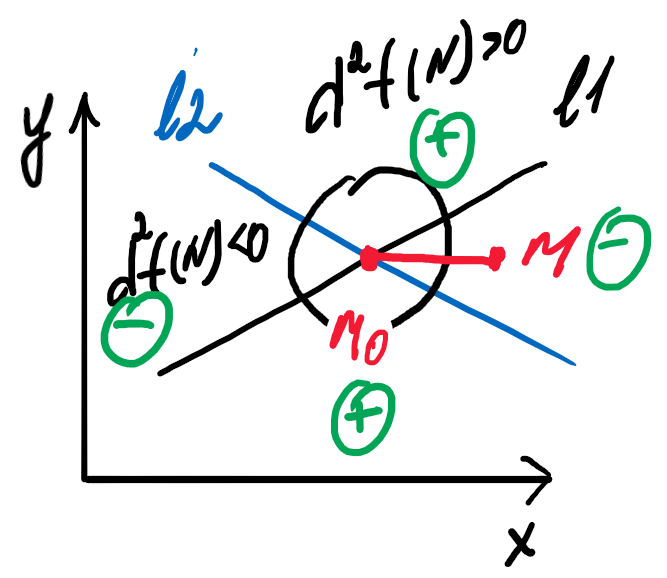
\includegraphics[width=35mm]{pictures/1_2_1.png}
                    \caption{}
                }
            \end{figure}
            \begin{align*}
                &l_1:\: (x - x_0) - \theta_1\,(y - y_0) = 0\\
                &l_2:\: (x - x_0) - \theta_2\,(y - y_0) = 0
            \end{align*}
            Таким образом мы видим
            \begin{align*}
                &\forall \varepsilon < \delta, \, \varepsilon > 0 \; & \exists M_1 \; d^2f(N_1) > 0 \; f(M) > f(M_1)\\
                & & \exists M_2 \; d^2f(N_2) > 0 \; f(M) < f(M_2)
            \end{align*}
        \end{enumerate}
    \end{Proof}

    \begin{Th}[Достаточное условие экстремума функции n - переменных]
        Пусть есть функция $u = f(M) = f(x_1, \dots, x_n) \in C^2(U(M_0))$ и $df(M_0) = 0$.\\
        Обозначим $d^2f(M_0) = \sum_{j = 1}^{n} \sum_{i = 1}^{n} a_{ij} dx_i dx_j, \, a_{ij} = a{ji}$\\
        Тогда
        \begin{enumerate}
            \item $d^2f(M_0) > 0 \Leftrightarrow \Delta_1 > 0, \dots, \Delta_n > 0 \Rightarrow M_0$ --- точка строгого минимума функции
            \item $d^2f(M_0) < 0 \Leftrightarrow \Delta_1 < 0, \dots, \Delta_2 > 0, \dots, (-1)^n\Delta_n \Rightarrow M_0$ --- точка строгого максимума функции
            \item $d^2f(M_0) \text{неопределённая форма} \Leftrightarrow \text{в} M_0$ --- нет экстремума функции
        \end{enumerate}
    \end{Th}
    \begin{Proof}
        Аналогино доказательству предыдущей теоремы, воспользуемся формулой Тейлора
        \[
            f(M) = f(M_0) + \frac{1}{1!} df(M_0) + \frac{1}{2!} d^2f(N), \, f(M) - f(M_0) = \frac{1}{2} d^2f(N)
        \]
        \begin{enumerate}
            \item \begin{align*}
                &\Delta_1(M_0) > 0, \dots, \Delta_n(M_0) > 0\\
                &\Rightarrow \text{ из критерия Сильвестра } \exists \delta>0 \; \forall N \in U_\delta(M_0)\\
                &\Rightarrow \; \Delta_1(N) > 0, \dots, \Delta_n(N) > 0\\
                &\Rightarrow \; d^2f(N) > 0\\
                &\Rightarrow \; f(M) > f(M_0), \; \forall M \in \mathring{U}_\delta(M_0) \Rightarrow M_0 \text{ --- точка минимума функции}
            \end{align*}
            \item Доказывается аналогично
            \item Принимаем без доказательств
        \end{enumerate}
    \end{Proof}

    \begin{Note}
        Если квадратичная форма равна нулю, то требуются дополнительные исследования. Например взятие производной  выше второй, рассмотрение точек в $\delta(M_0)$ окрестности 
    \end{Note}

    %\begin{Example}
    %    \textcolor{red}{!!!!!!!!!!}
    %\end{Example}

    %\begin{Example}
    %    \textcolor{red}{!!!!!!!!!!}
    %\end{Example}  %2   %OK  R
    \author{Andrei Tkachuk}

\section{Условные экстремумы ФНП}

\begin{Example}
    Найти экстремум для функции $u = x^2 + y^2$, ограниченной поверхностью $S: x + y = 1$\\
    \begin{figure}[h!]
        \noindent\centering{
            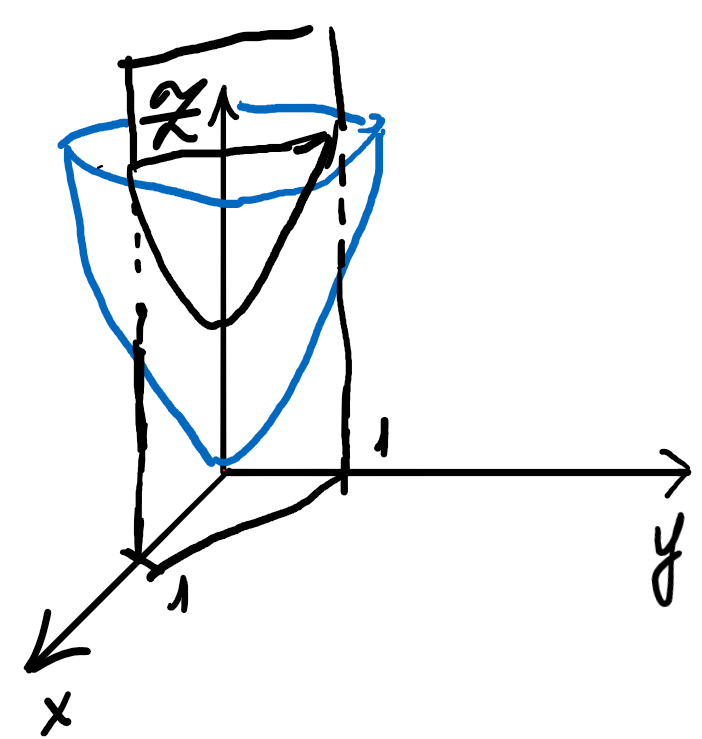
\includegraphics[width=35mm]{1_3_1.png}
            \caption{}
        }
    \end{figure}

    Решение
    \begin{align*}
        &y = 1 - x \; \Rightarrow \; u = x^2 + 1 + x^2 - 2x\\
        &u'_x = 4x - 2 = 0 &u''_x = 4 > 0\\
        &\begin{cases} 
                x = \frac{1}{2}\\
                y = \frac{1}{2}
        \end{cases} & \text{точек нет}
    \end{align*}
    Таким образом $M_0(\frac{1}{2}, \frac{1}{2})$ --- экстремум (строгий минимум)
\end{Example}
    В следующем примере предыдущий алгоритм не работает.
\begin{Example}
    Найти экстремум для функции $u = x$, ограниченной поверхностью $S: x^2 + y^2 = 1$\\
    \begin{figure}[h!]
    \noindent\centering{
        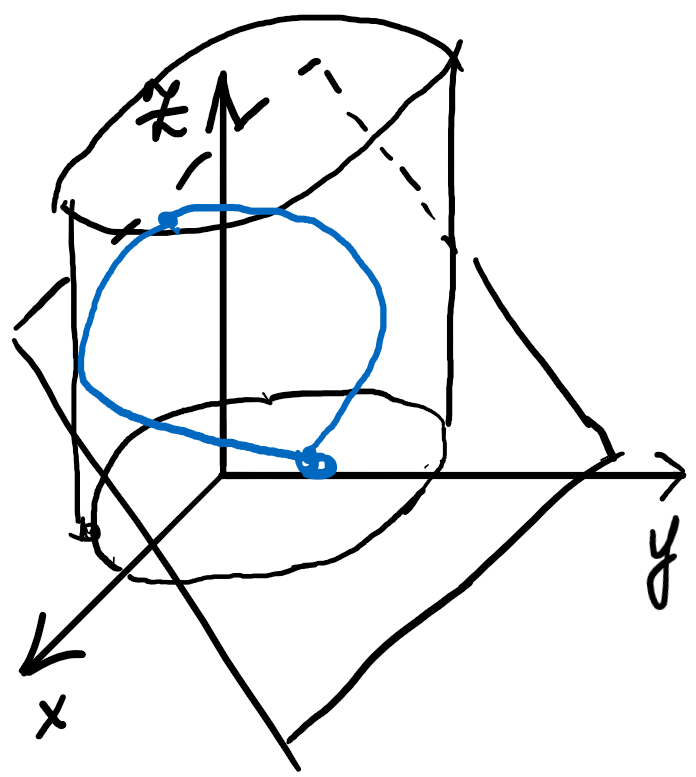
\includegraphics[width=35mm]{1_3_2.png}
        \caption{}
    }
    \end{figure}

    Если взять частную производную по $x$, то получим ($u'_x \neq 0$) что экстремум отсутствует, но по построению видно, что их два. Ошибка в том, что от "элипса" мы перешли к "отрезку" путём взятия производной.\\
    
    Чтобы избавиться от этого параметризируем $x$ и $y$ следующим образом
    \[
        \begin{cases}
        x = cos(t)\\
        y = sin(t) 
        \end{cases}
        t \in \bb{R}, \, t \in [0;\; 2\pi]
    \] 
    Тогда получим
    \begin{align*}
        &u = cos(t)\\
        &u'_t = -sin(t)\\
        &t_{min} = 0, \; t_{max} = \pi \text{, видно по построению}\\ 
        &u''_t = -cos(t)
    \end{align*}
    
\end{Example}
Таким образом, ключевым моментом является сохранение гладкости функции при взятии производных (т.е. если )

\begin{Note}[Условие связи. Условное]
    Условие свизи это функция(и) $\varphi_n(M)$, которая(ые) применяется(ются) к фукции $f(M)$, чтобы наложить ограничения (условия) на неё.
\end{Note}

\begin{Def}[Условный экстремум]
    Пусть $u = f(M) = f(x_1, \dots, x_n)$ определена в некоторой окрестности $U(M_0), \, M(x^0_1, \dots, x^0_n)$ и выполнено условие связи $S : \varphi_1(M) = 0, \dots, \varphi_k(M) = 0, \, M_0 \in S$. Тогда
        \begin{enumerate}
            \item $M_0$ --- точка локального условного минимума функции $f(M)$ при условии $M \in S \Leftrightarrow \exists \delta > 0 \; \forall M \in U_\delta(M_0) \cap S \; f(M) \geqslant f(M_0)$
            
            \item $M_0$ --- точка локального условного максимума функции $f(M)$ при условии $M \in S \Leftrightarrow \exists \delta > 0 \; \forall M \in U_\delta(M_0) \cap S \; f(M) \leqslant f(M_0)$
                        
            \item $M_0$ --- точка условного экстремума функции $f(M) \Leftrightarrow M_0$ точка условного минимума или условного максимума 
        \end{enumerate}
    Анлогичны будут рассуждения для строгого условного экстремума (помним, что он рассматривается в проколотой окрестности).
\end{Def}

\textcolor{cyan}{Повторимся, что условный экстремум отличается от обычного тем, что поиск ограничен $S$}

\begin{Def}[Формула Лагранжа задачи на усл. экстремум]
<<<<<<< HEAD
    Пусть $f(M), \varphi_1(M), \dots, \varphi_k(M)$ --- функции $n$ переменных $x_1, \dots, x_n$, определенных в $U(M_0)$. Тогда функция 
    \[
        L(M_i, \lambda) = f(M) + \lambda_1 \varphi_1(M) + \dots + \lambda_k \varphi_k(M)
    \] называется функцией Лагранжа задачи на условный экстремум функции $f(M)$ при условии $M \in S : \varphi_1 = \dots = \varphi_k = 0$
\end{Def}
\textcolor{cyan}{Формула Лагранжа позволяет связать функцию и дополнительное условие воедино, что очень удобно.}
=======
    Пусть $f(M), \varphi_1(M), \dots, \varphi_k(M)$ --- функции $n$ переменных $x_1, \dots, x_n$, определенных в $U(M_0)$. Тогда функция $L(M_i, \lambda) = f(M) + \lambda_1 \varphi_1(M) + \dots + \lambda_k \varphi_k(M)$ называется функцией Лагранжа задачи на условный экстремум функции $f(M)$ при условии $M \in S : \varphi_1 = \dots = \varphi_k = 0$
\end{Def}
\textcolor{cyan}{Формула Лагранжа позволяет связать функцию и дополнительное условие воедино, что очень удобно}
>>>>>>> 987ffbd49e869d463f80b3d5740cd957bfe1b037

\begin{Th}[Необходимый признак условного экстремума]
    Пусть 
    \[
        f(M), \varphi_1(M), \dots, \varphi_k(M) \in C^{-1}(U(M_0))
    \] 
    и $M_0$ --- внутренняя точка гладкой части поверхности $S$ 
    \[
<<<<<<< HEAD
    S: \varphi_1(M) = 0, \dots, \varphi_k(M) = 0, \quad M_0 \in S
=======
    S: \varphi_1(M) = 0, \dots, \varphi_k(M) = 0, \, M_0 \in S
>>>>>>> 987ffbd49e869d463f80b3d5740cd957bfe1b037
    \]
    Обозначим через 
    \[
        L(M, \lambda) = f(M) + \lambda_1\varphi_1(M) + \dots + \lambda_k\varphi_k(M)
    \]
    функцию Лагранжа задачи на условный экстремум функции $f(M)$, где $M \in S$. Тогда, если точка $M_0$ --- условный экстремум функции $f(M)$, то существует $\lambda_0(\lambda^0_1, \dots, \lambda^0_k)$, для которой
    \[
        dL(M_0, \lambda_0) = 0, \text{ где }  M_0(x^0_1, \dots, x^0_n), \; \lambda_0(\lambda^0_1, \dots, \lambda^0_k)
    \]
\end{Th}
\begin{Proof}
<<<<<<< HEAD
    Рассмотрим следующий случай: $n = 2, \, k = 1$ (размерность пространства и количество функций задающих поверхность), то есть $u = f(x, y), \; (x, y) \in U(M_0), \; M_0(x_0, y_0), \; M_0$ --- точка условного экстремума $S : \varphi(x, y) = 0$
    \begin{figure}[h!]
        \noindent\centering{
            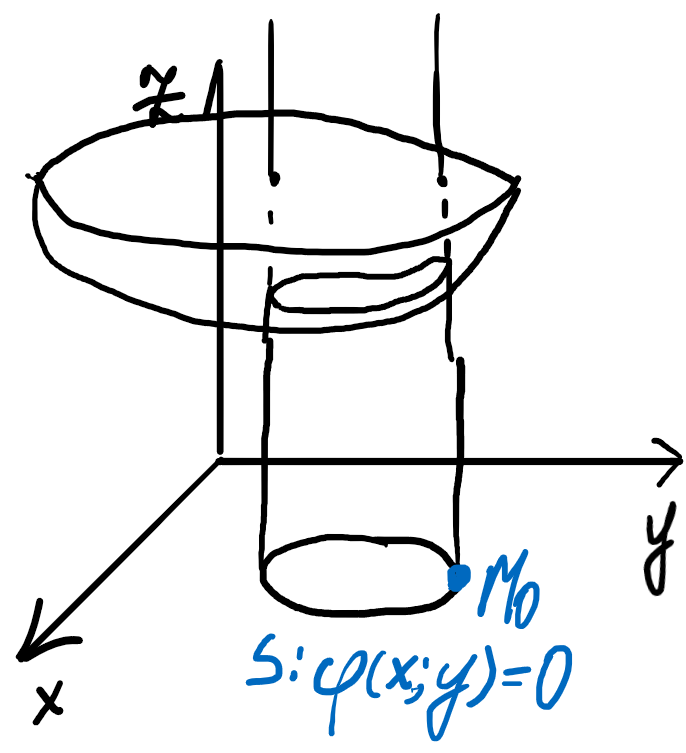
\includegraphics[width=35mm]{1_3_3.png}
            \caption{вместо z тут u}
=======
    Рассмотрим следующий случай: $n = 2, \, k = 1$ (размерность пространства и количество функций задающих поверхность), то есть $u = f(x, y), \; (x, y) \in U(M_0), \; M_0(x_0, y_0), \; M_0$ --- точка условного экстремума $S : \varphi(x, y) = 0$\\
    \begin{figure}[h!]
        \noindent\centering{
            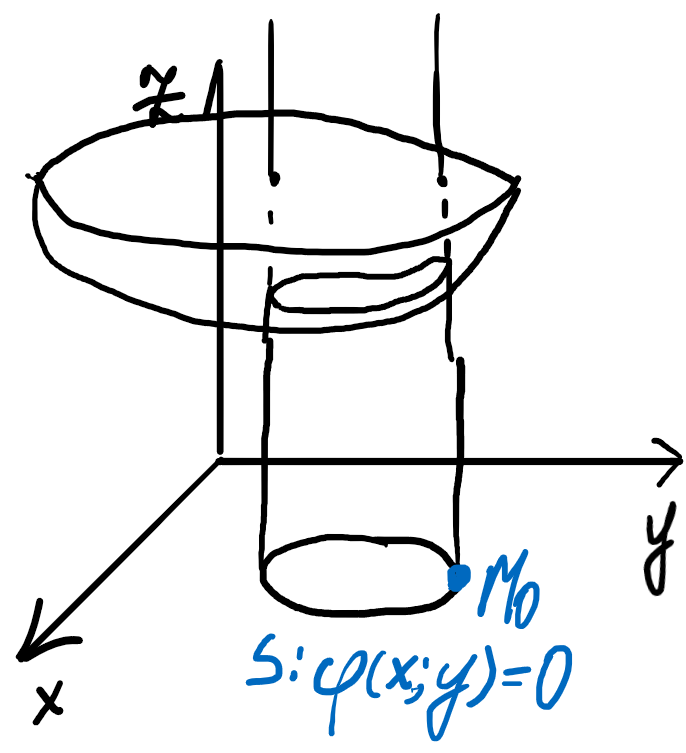
\includegraphics[width=35mm]{1_3_3.png}
            \caption{}
>>>>>>> 987ffbd49e869d463f80b3d5740cd957bfe1b037
        }
    \end{figure}\\
    Так как $\varphi(x, y)$ --- гладкая функция, то мы можем её параметризировать
    \[
<<<<<<< HEAD
        S :\: \begin{cases} 
            x = x(t)\\
            y = y(t)
          \end{cases} \quad t \in U(t_0)
    \]
    Тогда 
    \[
        M_0(x, y) = M_0(x(t_0), y(t_0)), \; x(t), \, y(t) \in C'(U(t_0))
    \]
    И следовательно по условию 
    \[
        \forall t \in U(t_0) \; \varphi(x(t), y(t)) = 0
    \]\\
    При этом $(x'(t_0), y'(t_0)) \neq (0, 0)$, то есть параметриация "хорошая" (Важность факта можно понять из примера 2).\\
    Таким образом задача на условный экстремум переходит в задачу на обычный экстремум функции $u = f(x(t), y(t))$ (таким образом получили функцию от одной переменной).\\
    По формуле частной производной
    \[
        u'(t) = f'_x\,x'_t+f'_y\,y'_t
    \]
    Аналогично для $\varphi'(t)$.\\
    Рассмотрим систему    
    \begin{align*}
        \begin{cases}
            f'_xx'_t+f'_yy'_t = 0\\
            \varphi'_xx'_t+\varphi'_yy'_t = 0
        \end{cases}
    \end{align*} 
    Так как $M_0$ - условный экстремум (по усл.), то $t_0$ - экстремум функции $u(t)$, значит $u'_t(t_0) = 0$, т.е. $t_0$ - решение первого уравнения системы. Причём мы имеем два решения: в $t_0$ и когда $x'_t,\; y'_t = 0$ (это справедливо, т.к. $(x'(t_0), y'(t_0)) \neq (0, 0)$)\\
    Так как по условию $\varphi(t) = 0$, то и $\varphi'(t) = 0$ для любого $t$. Значит, второе уравнение справедливо всегда.\\
    Получается по теореме Краммера следует
    \begin{gather*}
        \begin{pmatrix}
            f'_x & f'_y\\
            \varphi'_x & \varphi'_y
        \end{pmatrix} = 0 \Rightarrow \frac{f'_x(M_0)}{\varphi'_x(M_0)} = \frac{f'_y(M_0)}{\varphi'_y(M_0)} = -\lambda_0
    \end{gather*}
    \textcolor{cyan}{Примечание. Если знаменатель равен нулю, то и числитель будет ему равен. Поэтому всё ОК}\\
=======
        S \begin{cases} 
            x = x(t)\\
            y = y(t)
          \end{cases}, \; t \in U(t_0)
    \]
    При этом: $M_0(x(t_0), y(t_0)), \; x(t), \, y(t) \in C'(U(t_0))$.\\
    Из этого следует, что
    \[
        \forall t \in U(t_0) \Rightarrow \varphi(x(t), y(t)) = 0
    \]
    При этом $(x'(t_0), y'(t_0)) \neq (0, 0)$, то есть параметриация "хорошая" (Важность факта можно понять из примера 2).\\
    Таким образом задача на условный экстремум переходит в задачу на обычный экстремум функции $u = f(x(t), y(t))$\\
    \textcolor{red}{Почему мы можем устроить такой переход??? Т.е. до этого у нас была $\varphi(x, y)$ и её мы параметризировали. Или мы просто сказали, что x и y можно выразить через параметр (скорее всего да, но это странный довод)?}\\
    По формуле частной производной
    \[
        u'(t) = f'_xx'_t+f'_yy'_t
    \]
    Так как $M_0$ - условный экстремум (по усл.), то $t_0$ - экстремум $u(t) \Rightarrow u'_t(t_0) = 0$.
    
    \begin{align*}
        \begin{cases}
            f'_xx'_t+f'_yy'_t = 0\\
            \varphi'_xx'_t+\varphi'_yy'_t = 0 \textcolor{red}{\text{ откуда?}}
        \end{cases}
        \begin{pmatrix}
            f'_x & f'_y\\
            \varphi'_x & \varphi'_y
        \end{pmatrix}
          = \textcolor{red}{0} \Rightarrow \frac{f'_x(M_0)}{\varphi'_x(M_0)} = \frac{f'_y(M_0)}{\varphi'_y(M_0)} = -\lambda_0\\
          \textcolor{red}{\text{Почему определитель матрицы равен нулю?}}\\
        \text{Примечание. Если знаменатель равен нулю, то и числитель будет ему равен}
    \end{align*}
>>>>>>> 987ffbd49e869d463f80b3d5740cd957bfe1b037
    Таким образом из отношения можно получить следующию систему
    \[
        \begin{cases}
            f'_x(M_0) + \lambda_0\varphi'_x(M_0) = 0\\
<<<<<<< HEAD
            f'_y(M_0) + \lambda_0\varphi'_y(M_0) = 0
        \end{cases}
    \]
    Добавим ещё одно уравнение из условия, получим
    \[
        \begin{cases}
            f'_x(M_0) + \lambda_0\varphi'_x(M_0) = 0\\
            f'_y(M_0) + \lambda_0\varphi'_y(M_0) = 0\\
            \varphi(M_0) = 0
=======
            f'_y(M_0) + \lambda_0\varphi'_y(M_0) = 0\\
            \varphi(M_0) = 0 \textcolor{red}{\text{ тут не упущена производная?}}
>>>>>>> 987ffbd49e869d463f80b3d5740cd957bfe1b037
        \end{cases}
    \]
    Которая на самом деле ни что иное как
    \[
        \begin{cases}
            L'_x(M_0, \lambda_0) = 0\\
            L'_y(M_0, \lambda_0) = 0\\
<<<<<<< HEAD
            L'_\lambda(M_0) = 0
=======
            L_\lambda(M_0) = 0 \textcolor{red}{\text{ тут не упущена производная? Как определена эта функция?}}
>>>>>>> 987ffbd49e869d463f80b3d5740cd957bfe1b037
        \end{cases}
    \]
    Если мы сложим все три равенства то получим производную функции Лагранжа, которая равна нулю
    \[
        dL(M_0, \lambda_0) = 0
    \]
\end{Proof}

\begin{Th}[Необходимый признак усл. экстремума в общем случае]
    Пусть 
    \begin{gather*}
        \exists M(x_1, \dots, x_n), \, \exists M_0(x^0_1, \dots, x^0_n)\\
        f(M), \varphi_1(M), \dots, \varphi_k(M) \in C^2(U(M_0))\\
        L(M, \lambda) = f(M) + \lambda_1\varphi_1(M) + \dots + \lambda_k\varphi_k(M) 
    \end{gather*}
<<<<<<< HEAD
    и $\exists \lambda_0(\lambda^0_1, \dots, \lambda^0_k)$ для которой $ dL(M_0, \lambda_0) = 0 $ Рассмотрим
    \begin{gather*}
        S:\: d\phi_j(M_0) = 0 \quad j = 1, \dots, k\\
        S':\: \sum_{i=1}^{n} \frac{\delta\phi_j}{\delta x_j} \quad j = 1, \dots, k
    \end{gather*}
    $S'$ --- система $k$ линейных однородных уравнений относительно $n$ неизвестных $dx_1, \dots, dx_n$ размерность $m = n - r$, $r$ --- ранг матрицы поэтому $dx_1, \dots, dx_n$ -- независимые (свободные) переменные.\\
    Второй дифференциал 
    \[
        d^2L = \sum_{j = 1}^{n}\sum_{i = 1}^{n} \frac{\delta^2L(M_0, \lambda_0)}{\delta x_i\, \delta x_j}\, dx_i\, dx_j = q(dx_1, \dots, dx_m)
    \]
=======
    и $\exists \lambda_0(\lambda^0_1, \dots, \lambda^0_k)$ для которой 
    \[
        dL(M_0, \lambda_0) = 0
    \]
    \textcolor{red}{Дописать!!! Тут упущенны странные вещи с матрицами}\\
>>>>>>> 987ffbd49e869d463f80b3d5740cd957bfe1b037
    Тогда
    \begin{enumerate}
        \item $q > 0 \Rightarrow M_0$ --- точка строгого условного минимума функции
        
        \item $q < 0 \Rightarrow M_0$ --- точка строгого условного максимума функции
        
        \item $q$ --- неопределённая форма $\Rightarrow$ в $M_0$ нет экстремума 
    \end{enumerate}
\end{Th}
<<<<<<< HEAD

=======
>>>>>>> 987ffbd49e869d463f80b3d5740cd957bfe1b037
\begin{Proof}
    Принимаем без доказательств
\end{Proof}

\begin{Note}
    Условие $q > 0$ или $q < 0$ проверяется с помощью критерия Сильвестра. Данный факт используется для доказательства теоремы. 
\end{Note}

\begin{Note}
    По аналогии со вторым параграфом. Требуются дополнительные исследования, если второй диференциал равен нулю.
\end{Note}

\begin{Example}
    Дано:
    \[
        u = x^2 + y^2 + z^2 \quad S:\: x\,y + z = 2
    \]
    Решение:\\
    Поверхность $S$ можно описать одной гладкой функцией (т.е. $\phi = x\,y + z - 2$). Тогда получаем
    \begin{equation*}
        L = x^2 + y^2 + z^2 + 2\,\lambda\,(x\,y + z - 2)
    \end{equation*}
    Найдём частные производные
    \begin{gather*}
        L'_x = 2\,x - 2\,\lambda\,y = 0 \quad L'_y = 2\,y - 2\,\lambda\,x = 0 \quad L'_z = 2\,z - 2\,\lambda \\ L'_{\lambda} = xy + z - 2 = 0
    \end{gather*}
    Решаем систему и получаем следующие подозрительные точки
    \begin{align*}
        &M_0(0,\; 0,\; 2) && M_1(1,\; 1,\; 1) && M_2(-1,\; -1,\; 1)\\
        & \lambda_0 = 2 && \lambda_1 = 1 && \lambda_2 = -1
    \end{align*}
    Теперь требуется проверить точки на экстремумы. Найдём производные
    \begin{align*}
        &L''_{xx} = 2 && L''_{xy} = -2\,\lambda && L''_{xz} = 0 \\
        &L''_{yy} = 2 && L''_{yz} = 0\\
        &L''_{zz} = 2
    \end{align*}
    Дважды продифференцируем функцию Лагранжа. Помним, что $\lambda$ -- коэффициент. В итоге получаем
    \begin{gather*}
        d^2L = 2\,(dx)^2 + 2\,(dy)^2 + 2\,(dz)^2 - 4\lambda\,dx\,dy
    \end{gather*}
    Также $S':\: y\,dx + x\,dy + dz = 0$\\
    При подстановке $M_0$ и с помощью значений из $S'$ получаем значение функции Лагранжа.
    \[
        q_0 = 2\,(dx)^2 - 8\,dx\,dy + 2\,(dy)^2
    \]
    по критерию Сильвестра $q_0$ -- знакопеременна. Значит в $M_0$ нет экстремума.
    При $M_{1,2}$
    \[
        q_{1,2} = 4\,(dx)^2 + 4\,(dy)^2
    \]
    видим, что $M_{1,2}$ -- точка условного минимума
\end{Example}  %3   %OK  R
    \author{Andrei Tkachuk}

\section{Отыскание max и min значений для ФНП}

\begin{Example}
    Найти экстремумы для функции $u = x^2 + y^2$ ограниченной поверхностью $D: |x|+2|y| \leqslant 5$
    \begin{figure}[h!]
        \noindent\centering{
            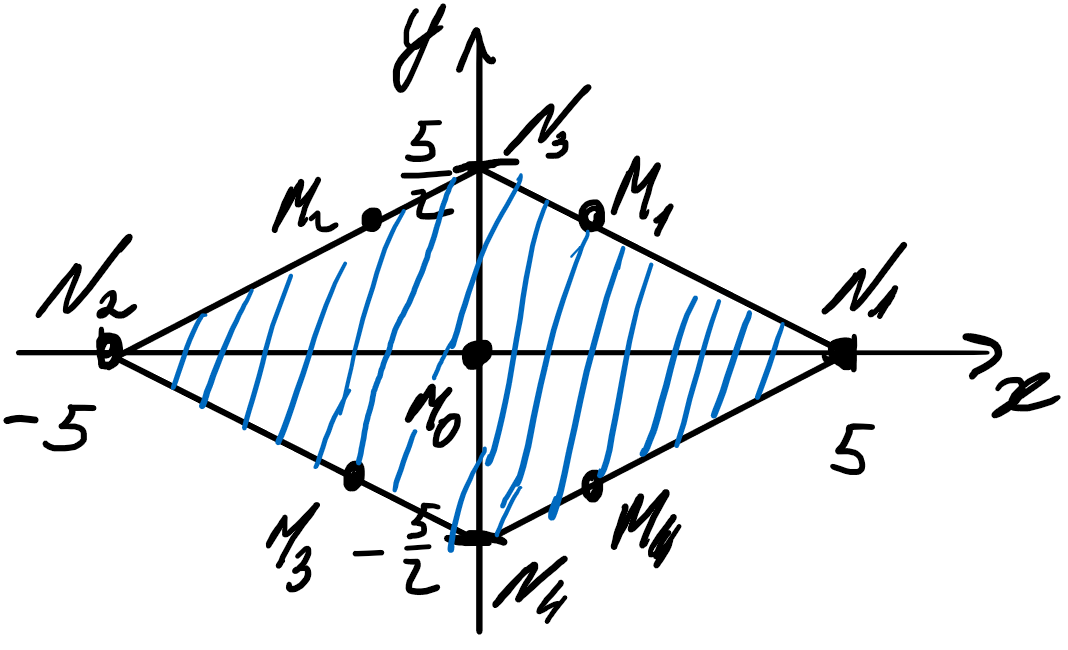
\includegraphics[width=50mm]{1_4_1.png}
            \caption{}
        }
    \end{figure}\\
    Таким образом, мы имеем дело с компактом (огр. множеством).
    \begin{enumerate}
        \item $u'_x = 2x = 0, \; u'_y = 2y = 0$\\
              $M_0(0, 0), \; u(M_0) = 0$ --- минимум
        \item Для удобства будем рассматривать первую четверть, так как компакт представляет собой ромб, который симметричен относительно осей (Замечание. Облатсть определена через 4 дифференцируемые функции).
        \begin{align*}
            &L_1 = x^2 + y^2 + \lambda(x + 2y - 5)\\
            &dL_1 = (2x + \lambda)dx + (2y + 2\lambda)dy + (x + 2y - 5)d\lambda = 0\\
            &\begin{cases}
                2x + \lambda = 0, \; x = -\frac{\lambda}{2}\\
                2y + 2\lambda = 0, \; y = -\lambda\\
                x + 2y = 5
            \end{cases}
        \end{align*}
        Подставим значения $x$ и $y$ в последнее уравнение, получим
        \[
            \lambda = -2
        \]
        следовательно экстремум в точке $M_1(1, 2)$\\
        Так как мы рассматриваем первую четветь, то в оставшихся трёх получим $M_2(-1, 2), \; M_3(-1, -2), \; M_4(1, -2)$\\
        Для данных точек значение функции 
        \[
            u(M_{1,2,3,4}) = 1 + 4 = 5
        \]
        \item Так как функция компакта не является гладкой, то рассмотрим следующие точки:
        \begin{align*}
            &N_1(5, 0), \; N_2(-5, 0) &N_3(0, \frac{5}{2}), \; N_4(0, -\frac{5}{2})\\
            &u(N_{1,2}) = 25  &u(N_{3,4}) = \frac{25}{4}
        \end{align*}
        Таким образом $u_{max} = u(N_{1,2}) = 25$.\\
        Окончательный ответ:
        \[
            \forall(x, y) \in D, \; 0 \leqslant u(x, y) \leqslant 25
        \]
    \end{enumerate}
\end{Example}

\begin{Note}[Как выглядит в общем случае]
    Пусть $u = f(x_1, \dots, x_n)$ определена в замкнутой односвязанной области $D : \varphi_1(M) \geqslant 0, \dots, \varphi_k(M) \geqslant 0$
    \begin{enumerate}
        \item $M \in \mathring{D}: \varphi_1(M) > 0, \dots, \varphi_k(M) > 0$\\
        Должно соблюдаться $f(M),\; \varphi_1(M),\; \dots,\; \varphi_k(M) \in C'(\mathring{D})$ --- гладкая по каждой части границы\\
        Для $df(M) = 0 \; \exists M_1, \dots, M_l \in \mathring{D}$ --- гладкая n-мерная часть
        
        \item Гладкая $(n-1)$ мерная часть границы $D$
        \begin{align*}
            &L_1 = f + \lambda_1\varphi_1&, &\dots,& &L_k = f + \lambda_k\varphi_k\\
            &dL_1 = 0& && & dL_k = 0\\
            &N_{1 1}, \dots, N_{1 l_1} + \lambda& && &N_{1 1}, \dots, N_{1 l_k} + \lambda
        \end{align*}
        $\varphi_1(N_{1 1}) = 0, \varphi_2(N_{1 1}) > 0, \dots, \varphi_k(N_{1 1}) > 0$
            
        \item Гладкая $(n-2)$ мерная часть границы $D$. Рассмотрим функции вида
        \[
            L = f(M) + \lambda_i\,\varphi_i(M) + \lambda_j\,\varphi_j(M)
        \]
        \begin{align*}
            S: &\varphi_i(M) = 0, &\varphi_j(M) = 0 \qquad (i \neq j)\\ 
            &1 \leqslant i \leqslant k  &1 \leqslant j \leqslant k\\
        \end{align*}
        Рассматриваем
        \[
            dL(M, \lambda_i, \lambda_j) = 0
        \]
        Получаем следующий набор точек $K_1,\; \dots,\; K_s$
        
        \item [\dots)]
        
        \item [n + 1)] Рассматриваем 0-мерное гладкое пространство (вершины или "плохие" точки). Получим следующее множетсво: $P_1,\; \dots,\; P_q$
    \end{enumerate}
    Таким образом, ответ:
    \begin{align*}
        U_{max} &= max\{u(M_1), \; \dots, \; u(P_q)\}\\
        U_{min} &= min\{u(M_1), \; \dots, \; u(P_q)\}
    \end{align*}
\end{Note}
\textcolor{cyan}{Тут надо написать обощающий алгоритм, т.е. что по факту для поиска экстремумов мы рассматриваем множества различных функций Лагранжа для различного количества границ.}  %4   %OK  R
    
    \author{Andrei Tkachuk}

\part{Обыкновенные дифференциальные уравнения и их системы}
\section{Введение. Дифференциальные уравнения 1-го порядка}

\begin{Def}[Дифференциальное уравнение]
    Уравнение вида $F(x, y, y', y'', \dots, y^{(n)}) = 0$ называют обыкновенным дифференциальным уранением n-го порядка. Решением называют функцию $y = y(x)$, которая n раз дифференцируема на интервале I: 
    \[
        F(x, y(x), y'(x), \dots, y^{(n)}(x)) = 0
    \]
\end{Def}

\begin{Def}[ДУ разрешённое относительно старшей производной]
    Если дифференциальное уравнение имеет вид
    \[
        y^{(n)} = f(x, y, y', \dots, y^{(n - 1)})
    \]
    то тогда его называют обыкновенным дифференциальным уравнением n-го порядка разрешённого относительно старшей производной 
\end{Def}

\begin{Example}[моделный]
    Пусть $f(x) \in C'_{(a, b)}, \, y' = f(x)$ --- дифференциальное уравнение n-го порядка, разрешённое относительно 1й производной.
    \begin{floatingfigure}[l]{50mm}
        \noindent
        \hfil
        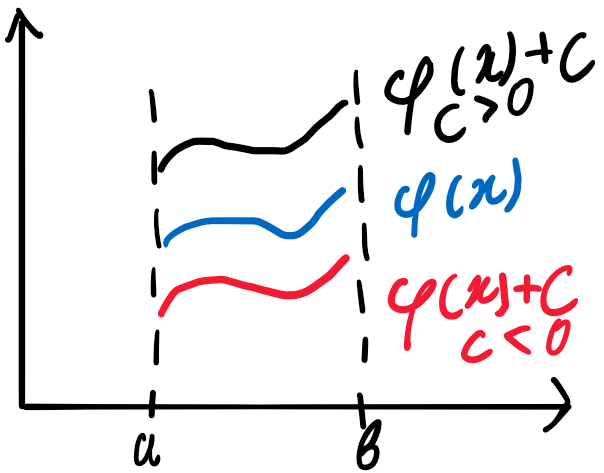
\includegraphics[width=45mm]{2_1_1.png}
        \hfil
    \end{floatingfigure}
    Если $y = y(x)$ решение, то
    \begin{gather*}
        y'(x) = f(x)\\ 
        y = \int{f(x)dx} + C = \varphi(x) + C \quad x \in (a, b)
    \end{gather*}
    Если $y = \psi(x)$ решение ДУ, то 
    \[
        \exists C,\; \forall x \in (a, b) \quad \psi = \varphi(x) + C
    \]
    Для любого $(x_0,\, y_0)$ в полосе, т.е. для $x_0 \in (a, b)$ существует решение $y = \varphi(x) - \varphi(x_0) + y_0, \, (y_0 \in \bb{R})$
\end{Example}

    Таким образом мы видим, что для одного дифференциального уравнения существует множетсво решений. Для конкретизации задачи используют условие Коши.

\begin{Def}[Задача Коши]
    Система вида
    \[
        \begin{cases}
            y' = f(x, y)\\
            y|_{x = x_0} = y_0 \quad (\text{конкретизация первообразной})
        \end{cases}
    \]
    Называется условием Коши, а задача о поиске решения это задача Коши
\end{Def}

    \begin{figure}[h!]
        \noindent\centering{
            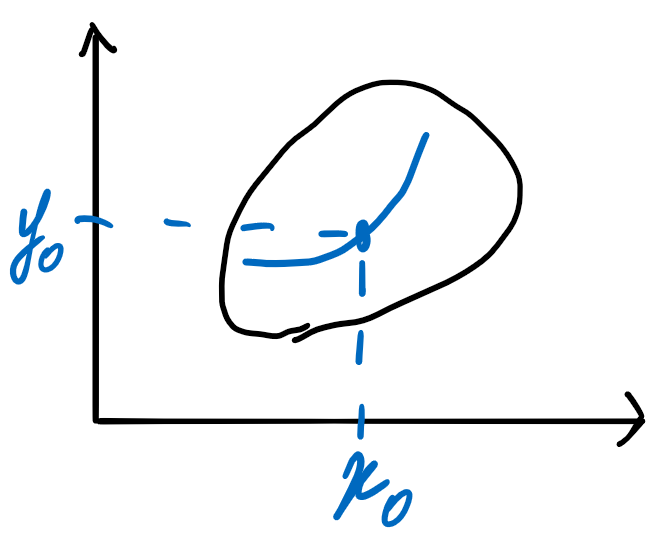
\includegraphics[width=55mm]{2_1_2.png}
            \caption{}
        }
    \end{figure}

\begin{Th}[Сущ. и ед. решения задачи Коши для ДУ 1го порядка]
    Пусть $f(x, y) \in C(U(M_0))$ и $\exists f'_y(M) \in C(U(M_0))$. Тогда существует такая $\delta > 0$ и существует решение $y' = y(x) \in U_\delta(M_0)$ задачи Коши c соответвующим условием $y' = f(x) \quad y(x_0) = y_0$ и такое решение в $U_\delta(x_0)$ единственно
\end{Th}
\begin{Proof}
    Принимаем без доказательств
\end{Proof}

\begin{Def}[Поле направлений ДУ]
    Пусть 
    \[
        y' = f(x, y), \quad f(x, y) \in C(D)
    \]
    $M_0(x_0, y_0)$ --- любая внутренняя точка области $D$. Запишем уравнение касательной к графику решения задачи Коши
    \[
        l_0 : Y-y_0 = f(x_0, y_0)\,(X-x_0)
    \]
    а задача Коши
    \[
        \begin{cases}
            y' = f(x, y)\\
            y|_{x = x_0} = y_0
        \end{cases}
    \]
    Пусть $\vec{\tau}$ --- единичный вектор касательной. Тогда множество $\{\vec{\tau}\}$ --- поле направлений
\end{Def}

\begin{figure}[h!]
    \noindent\centering{
        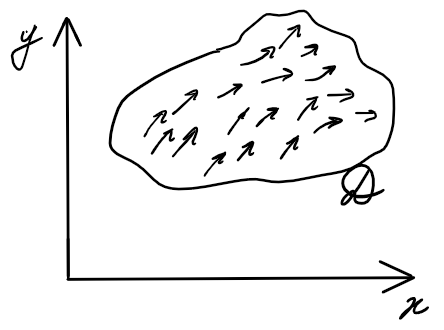
\includegraphics[width=55mm]{2_1_3.png}
        \caption{Поле направлений}
    }
\end{figure}

Вместе с понятием поля направлений вводят (для удобства) такую вещь как изоклины, т.е. линии, вдоль которых поле имеет одно и тоже направление. Задаётся уравнением $f(x, y) = C$\\

Тут важно заметить, что понятие поля направлений очень сильно связано с физикой, так как с помощью них можно легко описывать физические поля (эклектрическое, магнитное).

\textcolor{cyan}{С помощью полей направлений доказывается теорема о единственности задачи Коши.}

\begin{Example}
    Дано: 
    \[
        y' = \frac{y}{x}
    \]
    Требуется построить поле направлений.\\
    Решение.\\
    \begin{floatingfigure}[2]{34mm}
        \noindent
        \hfil
        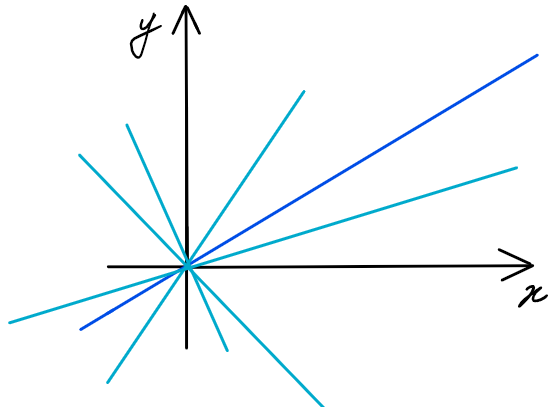
\includegraphics[height=24mm]{2_1_4.png}
        \hfil
    \end{floatingfigure}
    Изоклины для данного ДУ задаются уравнением 
    \[
        \frac{y}{x} = C
    \]
    
    Получается, изоклины представляют собой прямые, проходящие через начало координат. Уравнение изоклин $y = C\,x$. Если подставлять пары $(x,\; y)$, то мы заметим, что вектора поля направлений совпадают с изоклинами.\\
    Таким образом поле направлений состоит из множества прямых, проходящих через начало отсчёта (Точка (0, 0) выколотая).
\end{Example}

\begin{Example}
    Дано
    \[
        y' = -\frac{x}{y}
    \]
    Требуется построить поле направлений.\\
    Решение.\\
    Изоклины для данного ДУ задаются уравнением 
    \[
        -\frac{x}{y} = C
    \]
    Аналогично примеру выше, видим что изоклины проходят через начало координат.\\
    Рассмотрим несколько изоклин.
    \begin{enumerate}
        \item $C = -1$, тогда $y = x$. Прямая в первой и третьей четверти. Для неё значение углового коэфициента $k = -1$. Следовательно угол равен $\frac{3\,\pi}{4}$ для первой четверти
        
        \item Рассмотрим $C \in (-\infty;\, -1)$, тогда нетрудно заметить, что угол $\varphi$ соответственно изменялся для первой четверти от $\frac{\pi}{2}$ до $\frac{3\,\pi}{4}$ (оба не включительно).
        
        \item Рассмотрим $C \in (-1;\, 0)$. Тогда угол $\varphi$ соответственно изменялся для первой четверти от $\frac{3\,\pi}{4}$ до $\pi$.
    \end{enumerate}
    \begin{figure}[h!]
        \noindent\centering{
            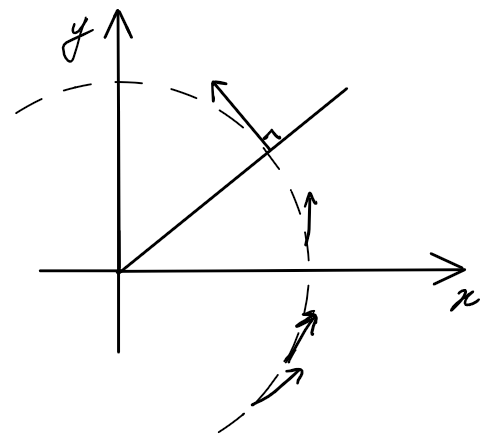
\includegraphics[width=45mm]{2_1_5.png}
            \caption{Иллюстрация примера}
        }
    \end{figure}
\end{Example}

\begin{Def}[Общее решение]
    Пусть $y' = f(x, y)$ --- ДУ первого порядка. Функция $y = \varphi(x, C)$ называется общим решением этого ДУ если:
    \begin{enumerate}
        \item $\forall C \in \bb{R}$ $y$ как функция от $x$ является решением ДУ
        
        \item Для любого решения $y = y^*(x)$ 
        \[
            \exists C^* \in \bb{R}, \quad y^*(x) \stackrel{(x)}{\equiv} \varphi(x, C^*)
        \]
    \end{enumerate}
\end{Def}

\begin{Note}
    Уравнение $\Phi(x, y, C) = 0$ --- называется общим интегралом ДУ. $y' = f(x, y)$ если:
    \begin{enumerate}
        \item всякая неявная функция $y = y(x, C)$ при фиксированном $C$ является решением ДУ
        \item всякое решение задаётся неявной функцией $y = y(x, C^*)$ для некоторого $C^*$
    \end{enumerate}
\end{Note}

\begin{Example}
    Для $y' = \frac{y}{x}$ очевидно из рисунка, что общее решение
    \[
        y = C \, x
    \]
\end{Example}

\begin{Example}
    Для $y' = -\frac{x}{y}$ очевидно из рисунка, что общий интеграл 
    \[
        x^2 + y^2 = C^2
    \]
    Общее решение отсутствует
\end{Example}

\begin{Note}
    Точка особая, если нарушается существование и единственность задачи Коши
\end{Note}

\begin{Note}
    $y = \varphi(x, C)$ --- <<общее>> решение, $y = \hat{y}(x)$ --- особое решение по отношению к общему решению.
\end{Note}

\begin{Note}
    Дано $y' = f(x)$, тогда 
    \[
        y = \int{f(x)\,dx} + C
    \] 
    называется решением ДУ <<в квадратурах>>.\\
    Важно заметить, что интегралов может быть несколько. Например,
    \[
        y^{(n)} = f(x)
    \] 
    интегрируется в квадратурах, через последовательное интегрирование. Другим примером является сумма интегралов.
\end{Note}  %5   %OK  
	\author{Andrei Tkachuk}

\section{ДУ в "дифференциалах". ДУ с разделяющимеся переменными}

\begin{Def}
    Пусть $M(x, y), N(x, y) \in C(D)$. Тогда уравнение вида
    \[
        M(x, y)dx + N(x, y)dy = 0
    \]
    называется ДУ в "дифференциалах" при этом
    \begin{enumerate}
        \item Решение этого ДУ - дифференциальные  уравнения $y = y(x), x \in I$, где $I$ --- отрезок, причём\\
        \[
            \forall x \in I \quad M(x, y(x)) + N(x, y(x))y'(x) = 0
        \]
        \item кривая линия $L : 
        \begin{cases}
            x = x(t)\\
            y = y(t)    
        \end{cases} t \in I$ --- называется интегральной кривой для данного ДУ. Это эквивалентно следующенму\\
        $L$ -- гладкая кривая и 
        \begin{multline*}
            \forall t \in I, \quad M(x(t), y(t))\,x'_t + N(x(t), y(t))\,y'_t = 0\\
            dx = x'_t\,dt, \; dy(t) = y'_t\,dt
        \end{multline*}
    \end{enumerate}
\end{Def}

\textcolor{red}{К чему замечание и два примера?}

\begin{Note}
    \begin{align*}
        y' = f(x, y) \qquad \Leftrightarrow \qquad f(x, y)dx - dy &= 0\\
        Mdx + Ndy &= 0 | \div dx\\
        M + Ny' &= 0\\
        y' &= -\frac{M}{N}
    \end{align*}
\end{Note}

\begin{Example} 
    Дано
    \[
        y' = \frac{y}{x}
    \]
    Тогда уравнение в <<диференциалах>>
    \[
        y\,dx - x\,dy = 0
    \]
    Только одна особая точка. Если $x = 0$, то интегральная кривая
\end{Example}

\begin{Example}
    Дано
    \[
        y' = -\frac{x}{y}
    \]
    Тогда уравнение в <<диференциалах>>
    \[
        y\,dy + x\,dx = 0
    \]
    Интегральные кривые --- замкнутые окружности
\end{Example}

\begin{Def}
    ДУ вида $f(x)\,dx = g(y)\,dy$ --- называется ДУ с разделёнными переменными. Причём $f(x) \in C(I),\; g(y) \in C(J)$.\\ $I,\; J$ --- интервалы
\end{Def}

\begin{Th}[Общий интеграл ДУ с разделяющимися переменными]
    В условиях определения выше пусть $F(x)$ первообразная к $f(x)$ на $I$, а $G(y)$ для $g(y)$ на $J$\\
    Тогда $F(x) = G(y) + C$ является общим интегралом ДУ $f(x)dx = g(y)dy$
\end{Th}
\begin{Note}
    В данной теореме мы просто говорим о взаимной связи первообразных с производными
\end{Note}
\begin{Proof}
    По условию:
    \[
        L: \begin{cases}
           x = x(t)\\
           y = y(t) 
        \end{cases} t \in (\alpha; \beta)
    \]
    Т.е. дана интегральная кривая ДУ $f(x)dx = g(y)dy$. Это эквивалентно
    \[
        \exists C \in \bb{R} \quad F(x(t)) = G(y(t)) + C    
    \]
    \begin{enumerate}
        \item [\textcolor{blue}{$\Rightarrow$}] Рассмотрим $f(x(t))\,x'_t = g(y(t))\,y'_t$. Тогда
        \begin{align*}
            f(x(t))\,x'_t &= g(y(t))\,y'_t\\
            (F(x(t)))'_t &= (G(y(t)))'_t \qquad  \text{Зам. }(F(x(t)))' = f(x(t))\,x'_t]\\
            (F(x(t)) - G(y(t)))'_t &= 0
        \end{align*}
        Так как производная равна нулю, то при взятии первообразных справа будет константа, получаем
        \[
            \exists C \equiv const \quad t \in (\alpha;\, \beta), \quad F(x(t)) = G(y(t)) + C
        \]
        
        \item[\textcolor{blue}{$\Leftarrow$}] Если $\forall t \in (\alpha; \beta) \; F(x(t)) = G(y(t)) + C$ то
        \begin{align*}
            [F(x(t))]'_t &= [G(y(t))]'_t + [C]'_t\\
            f(x(t))\,x'_t &= g(y(t))\,y'_t
        \end{align*}
        Таким образом $L$ --- интегральная кривая ДУ $f(x)\,dx = g(y)\,dy$
    \end{enumerate}
\end{Proof}

\begin{Note}
    Решение в "квадратурах":
    \[
        \int f(x)\,dx = \int g(y)\,dy + C
    \]
\end{Note}

\begin{Example}
    Дано $y\,dx - x\,dy = 0$. Решить ДУ.
   \begin{align*}
        y\,dx - x\,dy &= 0 \\
        \frac{dx}{x} &= \frac{dy}{y}\\
        \int\frac{dx}{x} &= \int\frac{dy}{y}\\
        \ln(|x|) &= \ln(|y|) - \ln(C_1) \qquad C = ln(C_1)\\
        y &= C\,x
   \end{align*}
   Ответ: $y = C\,x$
\end{Example}
\begin{Example}
    Дано 
    \[
        x\,dx - y\,dy = 0
    \] 
    Требуется решить ДУ.\\
    Решение
    \begin{gather*}
        x\,dx - y\,dy = 0\\
        \int x\,dx = -\int y\,dy
    \end{gather*}
    Для удобства возьмём константу $\frac{C^2}{2}$
    \begin{gather*}
        \frac{x^2}{2} = -\frac{y^2}{2} + \frac{C^2}{2}\\
        x^2+y^2 = C^2
    \end{gather*}
    Ответ: $x^2+y^2 = C^2$
\end{Example}

\begin{Def}
    ДУ вида 
    \[
        y' = f(x)g(x) \qquad f(x),\; g(y) \in C
    \] 
    называется ДУ с разделяющимися переменными
\end{Def}

\begin{Note} [Общий интеграл ДУ с разделяющимися переменными]
     Возьмём $y' \mapsto \frac{dy}{dx}$. Заменим $y'$ и умножим выражение из определения на $dx$, получим
    \begin{align*}
        y' &= f(x)\,g(y)\\
        \frac{dy}{dx} &= f(x)\,g(y)\\
        dy &= f(x)\,g(y)\,dx\\
        \frac{dy}{g(y)} &= f(x)\,dx\\
        \int \frac{dy}{g(y)} &= \int f(x)\,dx + C
    \end{align*}
    Таким образом, получили общий интеграл.\\
    
    \textcolor{cyan}{Замечание}. Было деление на $g(y)$. В общем случае также требуется рассматривать $g(y) = 0$
\end{Note}

\begin{Example}
    Дано
    \[
        y' = \frac{y}{x}
    \]
    Решение
    \begin{gather*}
        y' = \frac{y}{x}\\
        \frac{dy}{dx} = \frac{y}{x}\\
        \frac{dy}{y} = \frac{dx}{x}\\
        \int \frac{dy}{y} = \int \frac{dx}{x}\\
        \ln|y| = \ln|x| + \ln|C_1|\\
        y = C\,x
    \end{gather*}
\end{Example}

\begin{Example}
    Дано
    \[
        y' = -\frac{x}{y}
    \]
    Решение
    \begin{gather*}  
        y' = -\frac{x}{y}\\
        \frac{dy}{dx} = -\frac{x}{y}\\
        y\,dy = -x\,dx\\
        \int y\,dy = - \int x\,dx \\
        \frac{y^2}{2} = - \frac{x^2}{2} + \frac{C^2}{2}\\
        y^2 + x^2 = C^2
    \end{gather*}
\end{Example}

\begin{Def}
    ДУ 1го порядка приводящееся к ДУ с разделяющимися переменными
    \[
        y' = f(a\,x + b\,y + c) \qquad a\,b \neq 0, \quad f(z) \in C_{(I)}
    \]
\end{Def}

\begin{Note}
    Введём 
    \[
        z = a\,x + b\,y + C, \quad z = z(x)
    \]
    Тогда
    \begin{gather*}
        z' = a + b\,y' = [y' = f(z(x)) = f(x)] =  a + b\,f(x)\\
        z' = a + b\,f(x)\\
        \frac{dz}{dx} = a + b\,f(x)\\
        dx = \frac{dz}{a + b\,f(x)}\\
        x + C = \int \frac{dz}{a + b\,f(x)}
    \end{gather*}
    Получаем систему
    \[
        \begin{cases}
            x + C = \int \cfrac{dz}{a + b\,f(x)}\\
            z = a\,x + b\,y + C
        \end{cases}
    \]
    Отдельно требуется рассмотреть случай $a + b\,f(z) = 0$
\end{Note}

\begin{Example}
    Дано
    \[
        y' = \cos(x - y)
    \]
    Решение.
    \begin{align*}
        z &= x - y\\
        z' &= 1 - y' \qquad y' = cos(z)\\
        z' &= 1 - \cos(z) 
    \end{align*}
    Получили ДУ с разделяющимися переменными. Решаем
    \begin{align*}
        \frac{dz}{1- \cos(z)} &= dx\\
        \int \frac{dz}{1- \cos(z)} &= \int dx\\
        \int \frac{dz}{2\, \sin^2 \left(\frac{z}{2}\right)} &= x + C\\
        ctg\left(\frac{z}{2}\right) &= x + C
    \end{align*} 
    \begin{align*}
        z &= 2\,arctg(-x-C) + 2\,\pi\,k \qquad k \in \bb{N}\\
        x - y &= 2\,arctg(-x-C) + 2\,\pi\,k \qquad k \in \bb{N}\\
        y &= x - 2\,arctg(-x-C) - 2\,\pi\,k \qquad k \in \bb{N}
    \end{align*}
    Не забываем, что мы делили. Следовательно, требуется рассмотреть частный случай. $1 - cos(z) = 0$
    \begin{align*}
        1 - cos(z) &= 0\\
        cos(x - y) &= 1\\
        x - y &= -2\,\pi\,k \qquad k \in \bb{N}\\
        y &= x + 2\,\pi\,k \qquad k \in \bb{N}
    \end{align*} 
    Проверим является ли значение выше упущенным решением.
    \begin{align*}
        y'& = 1 \qquad (\text{производная взята из равенства выше})\\
        cos(x - y) &= cos(-2\,\pi\,k) = 1 \qquad (\text{подстановка в  условие})
    \end{align*}
    Левая и правая части условия равны, следовательно $y = x + 2\,\pi\,k$ входит в множество решений.
    
    \pagebreak
    
    Множество решений выглядит следующим образом
    \begin{figure}[h]
        \noindent\centering{
            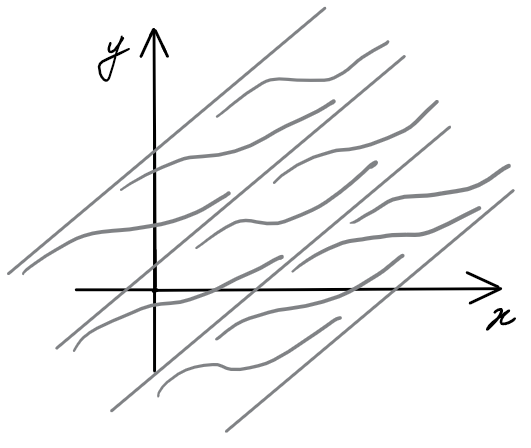
\includegraphics[width=55mm]{2_2_1.png}
            \caption{}
        }
    \end{figure}
\end{Example}  %6   %OK  
    \author{Tkachuk Andrei}

\section{Однородные ДУ первого порядка}

\begin{Def}
    Пусть функция $f(t)$ определена и непрерывна на некотором интервале и $f(t)\; \cancel{\equiv}\; t$. Тогда ДУ 
    \[
        y' = f\left(\frac{y}{x}\right)
    \]
    называются однородными ДУ первого порядка.
\end{Def}

\begin{Note}
    $F(x_1, \dots, x_n)$ называются однородными функциями веса $k$, если 
    \[
        \forall t \in \bb{R} \; F(t\,x_1, t\,x_2, \dots, t\,x_n) = t^k\,F(x_1, x_2, \dots, x_n)
    \]
    
    Пример. $f(\frac{t\,y}{t\,x}) = f(\frac{y}{x})$ --- однородное ДУ веса $k = 0$
\end{Note}
\begin{Note} [Как решить однородное ДУ]
    Дано 
    \[
        y' = f\left(\frac{y}{x}\right)
    \]
    Введём 
    \[
        t(x) = t = \frac{y}{x}
    \]
    Тогда
    \textcolor{red}{тут опечатка?}
    \[
        y = t\,x, \quad y' = t'\,x + t = f(t)
    \]
    Таким образом получаем ДУ с разделяюмися переменными
    \[
        t' = \frac{f(t) - t}{x}
    \]
    Решаем
    \[
        \frac{dt}{dx} = \frac{f(t) - t}{x}
    \]
    Так как мы будем делить на $f(t) - t$, то потребуется рассмотреть два случая
    \begin{align*}
        &1) f(t) - t \neq 0& &2) f(t) - t = 0&\\
        &\int\frac{dt}{f(t) - t} = \int \frac{dx}{x}& &\exists\alpha \in \bb{R} \quad f(\alpha) = \alpha, \quad y = \alpha\,x&\\
        &ln(|x|) = \int \frac{dt}{f(t) - t} + ln(C)& &y'=\alpha= f(\alpha) = f\left(\frac{x}{y}\right)&\\
        &\begin{cases}
            x = Ce^{\int \frac{dt}{f(t) - t}}\\
            y = t\,x
        \end{cases}&
    \end{align*}
\end{Note}

\begin{Example}
    Дано
    \[
        y' = \frac{x\,y + y^2}{x^2}
    \]
    Решение.
    \[
        y' = \frac{x\,y + y^2}{x^2} = \frac{y}{x} + \left(\frac{y}{x}\right)^2\\
    \]
    Делаем замену
    \begin{gather*}
            t = \frac{y}{x}, \quad y = t\,x \quad dy = x\,dt + t\,dx\\
            \frac{dy}{dx} = y' = \frac{x\,dt}{dx} + t = t'\,x + t
    \end{gather*}
    Подставляем и получаем
    \begin{gather*}    
        t'\,x + \cancel{t} = \cancel{t} + t^2\\
        \frac{dt}{t^2} = \frac{dx}{x}\\
        -\frac{1}{t} = \ln|x| - \ln(C) = - \frac{x}{y}\\
        \frac{x}{y} = \ln\left(\frac{C}{x}\right) \qquad C \neq 0\\
        y = \cfrac{x}{\ln\left(\cfrac{C}{x}\right)} \qquad C \neq 0
    \end{gather*}
    Также требуется рассмотреть частный случай, когда $t = 0$, тогда $y = 0$
\end{Example}

\begin{Note}
    Дано:
    \[
        y' = f\left(\frac{a_1\,x + b_1\,y + c_1}{a_2\,x + b_2\,y + c_2}\right)
    \]
    где 
    \[
        \begin{vmatrix} a_1 & b_1 \\ a_2 & b_2\end{vmatrix} \neq 0 \quad c_1^2 + c_2^2 \neq 0
    \]
    Вопрос. Как превести эту дробь к однородному ДУ 1-го порядка? $f\left(\frac{y}{x}\right)$\\
    Ответ:\\
    Рассмотрим систему
    \[
        \begin{cases}
            a_1\,x + b_1\,y + c_1 = 0\\
            a_2\,x + b_2\,y + c_2 = 0
        \end{cases} \Delta = \begin{vmatrix} a_1 & b_1 \\ a_2 & b_2\end{vmatrix} \neq 0\\
    \]
    Тогда по теореме Крамера получим, что существует единственное решение $(\alpha;\; \beta)$ этой системы линейных алгебраических уравнений.\\
    Сделаем замену
    \[
    \begin{cases}
        x = x_1 + \alpha\\
        y = y_1 + \beta
    \end{cases}
    \]
    Получим
    \begin{align*}
        a_1\,x + b_1\,y + c_1 &= a_1(x_1 + \alpha) + b_1(y_1 + \beta) + c_1 = \\
        &=a_1\,x_1 + b_1\,y_1 + \underbrace{a_1\,\alpha + b_1\,\beta + c_1}_{0 \text{ (как корни ур-я)}} = \\
        &=a_1\,x_1 + b_1\,y_1
    \end{align*}
    Помимо этого, если взять диференциалы от заменённых функций, получим
    \[
        \begin{cases}
            dx = dx_1\\
            dy = dy_1
        \end{cases}
    \]
    Таким образом мы можем перейти к отношению линейных функций. Из первоначального уравнения получаем.
    \begin{multline*}
        y' = \frac{dy}{dx} = \frac{dy_1}{dx_1} = f\left(\frac{a_1\,x + b_1\,y + c_1}{a_2\,x +  b_2\,y + c_2}\right) = f\left(\frac{a_1\,x_1 +  b_1\,y_1}{a_2\,x_1 + b_2\,y_1}\right) =\\
        = f\left(\frac{a_1 +  b_1\,\frac{y_1}{x_1}}{a_2\,x_1 + b_2\,\frac{y_1}{x_1}}\right) = g\left(\frac{y_1}{x_1}\right)
    \end{multline*}
    Таким образом
    \[
        \frac{dy_1}{dx_1} = g\left(\frac{y_1}{x_2}\right)
    \]
    получили однородное ДУ 1-го порядка, где 
    \[
        \begin{cases}
            x_1 = x - \alpha\\
            y_1 = y - \beta
        \end{cases}
    \]
\end{Note}

\begin{Example}
    Дано
    \[
        y' = \frac{x + y + 1}{x - y}
    \]
    Решение.
    \begin{enumerate}
        \item Найдём коэфициенты $\alpha$ и $\beta$. Для этого рассмотрим систему.
        \[
            \begin{cases}
                \alpha + \beta + 1 = 0\\
                \alpha - \beta = 0
            \end{cases} \qquad \text{Получаем } \alpha = \beta = -\frac{1}{2}
        \]
        
        \item Зная $\alpha$ и $\beta$ Делаем замену $x$ и $y$ на
        \[
            x = x_1 - \frac{1}{2} \qquad y = y_1 - \frac{1}{2}
        \]
        Получаем
        \begin{align*}
            y' = \frac{x + y + 1}{x - y} &= \frac{x_1 + y_1}{x_1 - y_1}\\
            \frac{dy_1}{dx_1} &= \frac{x_1 + y_1}{x_1 - y_1}
        \end{align*}
        
        \item Пусть $t = \frac{y_1}{x_1}$, следоватнльно $y_1 = t\,x_1$. Тогда 
        \[
            dy_1 = x_1\,dt + t\,dx_1 \quad \Rightarrow \quad \frac{dy_1}{dx_1} = \frac{dt}{dx_1}\,x_1 + t
        \]
        А после замены $y_1 = t\,x_1$ справа получаем
        \[
            \frac{x_1 + t\,x_1}{x_1 - t\,x_1} = \frac{1 + t}{1 - t}
        \]
        Таким образом
        \begin{align*}
            \frac{dt}{dx_1}\,x_1 + t &= \frac{1 + t}{1 - t}\\
            \frac{dt}{dx_1}\,x_1 &= \frac{1 + t - t + t^2}{1 - t}\\
            \frac{1 - t}{1 + t^2}\,dt &= \frac{dx_1}{x_1}\\
            \int \frac{1 - t}{1 + t^2}\,dt &= ln|x_1|
        \end{align*}
        После интегрирования получаем
        \[
            \ln|x_1| + C_1 = arctg(t) - \frac{1}{2}\,\ln|1 + t^2|\\
        \]
        Делаем обратную замену $t = \frac{y_1}{x_1}$, получаем
        \begin{gather*}
            \ln|x_1| + C_1 = arctg\left(\frac{y_1}{x_1}\right) - \frac{1}{2}\,\ln\left|1 + \left(\frac{y_1}{x_1}\right)^2\right|\\
            \cancel{\ln|x_1|} + C_1 = arctg\left(\frac{y_1}{x_1}\right) - \frac{1}{2}\,\ln|x_1^2 + y_1^2| + \cancel{\ln|x_1^2|}\\
        \end{gather*}
        Ответ
        \[
            arctg\left(\frac{y_1}{x_1}\right) - \frac{1}{2}\,\ln|x_1^2 + y_1^2| = C
        \]
    \end{enumerate}
\end{Example}  %7   %OK  
    \section{Линейные дифференциальные уравнения. ДУ Бернулли}

\begin{Def}[Линейное ДУ]
    ДУ вида 
    \[
        a(x)\,y' + b(x)\,y + c(x) = 0
    \] 
    называется линейным диференциальным уравнением, а\\
    \[
        y'+p(x)\,y=q(x)
    \]
    является приведённой формой линейного ДУ первого порядка, где
    \[
        p(x)\in C_{(a;\;b)} \quad q(x) \in C_{(a;\;b)}
    \]
\end{Def}

\begin{Def}
    Пусть 
    \begin{align}
        y'+p(x)\,y&=q(x)\\
        y'+p(x)\,y&=0
    \end{align}
    ДУ $(2)$ - линейное однородное ДУ, соответствующее линейному ДУ $(1)$\\
\end{Def}

\begin{Note}
Метод Лагранжа для решения линейных неоднородных ДУ первого порядка, в вариации произвольной постоянной\\
Дано
\[
    y'+p(x)\,y=q(x)
\]
Решение
    \begin{enumerate}
        \item Ищем решение для однородного уравнения
        \begin{align*}
            y'+p(x)\,y&=0\\
            \frac{dy}{y}&=-p(x)\,dx\\
            \ln(y)&=-\int p(x)\,dx+\ln(C)\\
            y&= C\,v(x)
        \end{align*}
        Замечание. $v(x)=e^{-\int p(x)\,dx}$\\
        Таким образом, получили \textbf{частное} решение для однородного ДУ.
    
        \item ищем решение первоначального ДУ в виде $y=C(x)\,v(x)$, где\\ $C(x)$ --- постоянная, зависящая от $x$ (произвольная постоянная)
        \begin{align*}
            y = C(x)\,v(x)\\
            y'=C'\,v + C\,v'
        \end{align*}
        Подставим в уравнение из условия
        \begin{align*}  
            C'\,v+C\,v'+p\,C\,v&=q\\ 
            C'\,v+C\,(v'+p\,v)&=q
        \end{align*}
        Так как на первом шаге мы рассматривали $v'+p\,v = 0$, то уравнения выше получаем
        \begin{align*}
            C\,(v'+p\,v)&=0\\
            C'\,v(x) &= q(x)\\
            C'&=\frac{q(x)}{v(x)}\\
            C(x)&=\int \frac{q(x)}{v(x)}\,dx+const
        \end{align*}
        Подставим значение $v(x)$ из шага 1, получим
        \[
            C(x) = \int q(x)\,e^{\int p(x)\,dx}\,dx+const \qquad x \in (a;\,b)
        \]
        Или
        \[
            C(x) = u(x) + const
        \]
        \item полное решение ДУ имеет вид
        \[
            y= C(x)\,v(x) = (u(x) + C)\,v(x)=u(x)\,v(x)+C\,v(x)
        \]
        В общем виде
        \[
            y=y_{(\text{частное решение неоднородного})} + C\,y_{(\text{частное решение однородного})}
        \]
    \end{enumerate}
\end{Note}

\begin{Note}[По поводу решения задач Коши]
    Пусть 
    \[
        p(x),\; q(x)\in C_{(a;\,b)}, \quad x_0 \in (a;\,b), \quad y_0 \in \bb{R}
    \]
    Тогда задача Коши\\
    \[
        \begin{cases}
            y'+p(x)y=q(x) \\
            y'|_{x=x_0}=y_0
        \end{cases}
    \]
    имеет единственное решение, определённое на $(a;\;b)$ вида\\
    \[
        y=\underbrace{e^{-\int_{x_0}^{x} p(t)dt}}_{v(x)}\,\left(\underbrace{y_0}_{c}+\underbrace{\int_{x_0}^{x}\underbrace{g(s)e^{\int_{x_0}^{s} p(t)dt}ds}_{\frac{g(s)}{v(s)}}}_{u(x)}\right)
    \]
\end{Note}

\begin{Example}
    Дано
    \[
        xy'+y=3x^3
    \]
    Решение.\\
    Делим на $x$ получим
    \[
        y'+\frac{y}{x}=3x^2
    \]
    \begin{enumerate}
        \item Решаем однородное уравнение. Находим решение для $\mathring{y} = v(x)$
        \begin{align*}
            v'+\frac{v}{x}&=0\\
            \frac{dv}{v}&=-\frac{dx}{x}\\
            \ln(v)&=-\ln(x)+\ln(C)\\
            v&=\frac{C}{x} \text{ --- общее решение}\\
            \text{При } C=1 \quad v(x)&=\frac{1}{x} \text{ --- частное решение}
        \end{align*}
        
        \item Решаем общее уравнение. где $y = C(x)\,v(x) = v(x)\,u(x)$ 
        \[
            \text{Так как } y=\frac{u}{x} \text{, то } y'=\frac{u'}{x} - \frac{u}{x^2}
        \]
        Подставляем в первоначальное уравнение. Получаем
        \begin{align*}
            \frac{u'}{x} - \frac{u}{x^2}+\frac{u}{x^2}&=3x^2\\
            u'&=3x^3\\
            u(x)&=\frac{3}{4}x^4+c
        \end{align*}

        \item Совмещаем результаты шагов 1 и 2. Получаем ответ
        \[
            y=\frac{3}{4}\,x^4+\frac{c}{x} \qquad x\in \bb{R}
        \]
    \end{enumerate}
\end{Example}

\begin{Def}
    ДУ вида 
    \[
        y'+p(x)\,y=q(x)\,y^\alpha \qquad \alpha \in \bb{R} \setminus \{0;\,1\}
    \]
    называется ДУ Бернулли
\end{Def}

\begin{Note}[Решение ДУ Бернулли]
    ДУ Бернулли интегрируется методом Лагранжа в вариации произвольной постоянной
    \begin{enumerate}
        \item Ищем $v = v(x)$ частное решение соответствующее линейному однородному ДУ
        \begin{align*}
            v'+p(x)\,v &=0\\
            v(x) &=e^{-\int p(x)\,dx}
        \end{align*}
        
        \item Ищем общее решение ДУ для $u =u (x)$, где $y=u(x)\,v(x)$
        \begin{gather*}
            u'\,v+\underbrace{u(v'+pv)}_{=0 (\text{см. зам. 2})}=qu^{\alpha}v^{\alpha}\\
            u'\,v(x)=q(x)u^{\alpha}v^{\alpha}(x)
        \end{gather*}
        Замечание. Нам известно то, что с аргументом.\\
        Далее разделим на $u^{\alpha}\,v(x)$
        \begin{align*}
            \frac{du}{u^\alpha}&=q(x) \, v^{\alpha-1}(x)\,dx\\
            \int \frac{du}{u^\alpha}&=\int q(x)\, v^{\alpha-1}(x)\, dx\\
            \frac{u^{1-\alpha}}{1-\alpha} &=\int q(x)\,v^{\alpha-1}(x)\,dx + C\\
            u = u(x,\;C) &= \left((1-\alpha)\left(\int q(x)\, v^{\alpha-1}(x)\,dx+C\right)\right)^{\frac{1}{1-\alpha}}
        \end{align*}
        \item Таким образом, ответ
        \[
            y=u(x,\;C)\,v(x)
        \]
    \end{enumerate}
\end{Note}

\begin{Example}
    Дано
    \[
        x\,y'-y=x\,y^2
    \]
    Решение.\\
    Для соответсвия ДУ Бернулли разделим на $x$. Получим
    \[
        y'-\frac{y}{x}=y^2
    \]
    Видим, что
    \[
        p(x)=-\frac{1}{x}, \quad q(x)=1, \quad \alpha=2
    \]
    \begin{enumerate}
        \item Ищем частное решение однородного ДУ 
        \begin{gather*}
            v'-\frac{v}{x}=0\\
            \frac{dv}{v}=\frac{dx}{x}\\
            \ln|v|= - \ln|x|+ \ln(C)\\
            v=C\,x
        \end{gather*}
        Если $C=1$, то получаем частное решение $v(x)= x$
        
        \item Рассмотрим $y=u(x)\,v(x)=u\,x$\\
        Подставим в уравнение из условия, получим
        \begin{gather*}
            u'\,x+u-u=u^2\,x^2\\
            u'=u^2\,x\\
            \frac{du}{u^2}=x\,dx\\
            -\frac{1}{u}=\frac{x^2}{2} - C\\
            u = \cfrac{1}{C-\cfrac{x^2}{2}}
        \end{gather*}
        
        \item Ответ
            \begin{align*}
                y &= \cfrac{x}{C-\cfrac{x^2}{2}}\\
                y &= \frac{2\,x}{2\,C-x^2}
            \end{align*}
    \end{enumerate}
\end{Example}
















  %8   %OK  Q
    \section{ДУ в полных дифференциалах}
\begin{Def}
    ДУ вида
    \[
        M(x,\;y)\,dx+N(x,\;y)\,dy=0 \qquad M(x,\;y),\; N(x,\;y)\in C'(D)
    \] 
    называется ДУ <<в полных дифференциалах>>, если $\exists F(x,\;y) \in C^2(D)$ для которой
    \begin{gather*}
        F'_x=M(x,\;y)\\
        F'_y=N(x,\;y)
    \end{gather*}
    то есть ДУ имеет вид $dF(x,\;y)=0$\\
    
    \textcolor{cyan}{Примечание.} Дифференциал \[dF(x,\;y)=F'_x\,dx+F'_y\, dy=M\,dx+N\,dy\] является полным, поэтому и название уравнения <<в полных дифференциалах>>.
\end{Def}

\begin{Th}[Об общем интеграле]
    В условиях определения 1, уравнение $F(x,\;y) = C$ даёт общий интеграл ДУ $dF(x,\;y)=0$ (предполагаем, что D-односвязная область (ограниченная простой замкнутой кривой))
\end{Th}

\begin{Proof}
    Интегральная кривая $dF(x,\, y) = 0$
    \begin{gather*}
        L:
        \begin{cases}
            x=x(t)\\
            y=y(t) 
        \end{cases} \quad t\in I\\
        \Leftrightarrow\\
        \exists C = const, \quad \forall t \in I, \quad F(x(t),\, y(t))= C
    \end{gather*}
    \begin{enumerate}
        \item[\textcolor{blue}{$\Rightarrow$}]
        По условию имеем
        \[
            F_x'(x(t),\,y(t))\,x'_t+F_y'(x(t),\,y(t))\,y'_t=0
        \]
        Значит
        \begin{align*}
            &(F(x(t),y(t)))'=0, \quad t \in I\\
            \Rightarrow \; &\exists C = const \quad \forall t \in I \quad F(x(t),\, y(t)) = C
        \end{align*}
        
        \item[\textcolor{blue}{$\Leftarrow$}] По условию 
        \[
            \forall t \in I \quad F(x(t),\, y(t))= C
        \]
        Продиференцируем равенство, получим
        \[
            F_x'\,x'_t + F_y'\,y'_t = 0
        \]
        По определению следует, что\\
        $L$ --- интегральная кривая ДУ $F_x'\,dy+F_y'\,dx = 0$ и значит $dF(x,y)=0$
    \end{enumerate}
\end{Proof}

\begin{Note}[решение задачи Коши]
    \[
        \begin{cases}
            dF(x,y)=0\\
            y|_{x=x_0}=y_0
        \end{cases}
    \]
    $F(x,y)=F(x_0,y_0)$ (в неявном виде)\\
\end{Note}

\begin{Example}
    Дано
    \[
        F(x,y)=x^2 
    \]
    \textcolor{red}{Что ищем?}\\
    Решение.
    \begin{align*}
        F'_x &=2\,x\,y\\
        F'_y &= x^2
    \end{align*}
    Тогда уравнение <<в полных диференци-алах>> будет выглядеть так
    \begin{floatingfigure}[l]{50mm}
        \noindent
        \hfil
        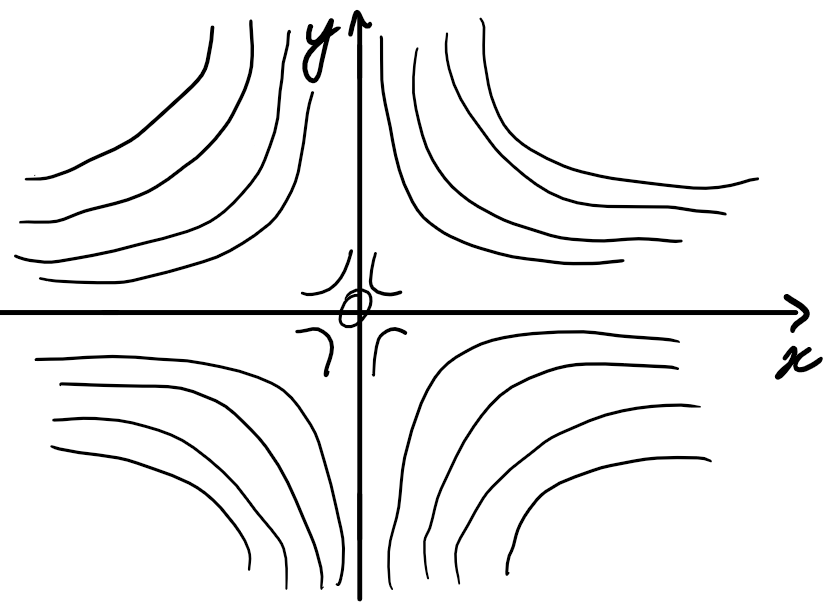
\includegraphics[width=45mm]{2_5_1.png}
        \caption{Общее решение}
        \hfil
    \end{floatingfigure}
    \begin{gather*}
        2\,x\,y\,dx+x^2\,dy = 0\\
        x^2\,y + x^2\,y = C_1\\
        x^2\,y = C = \frac{C_1}{2}
    \end{gather*}
    Общее решение
    \[
        y=\frac{C}{x^2}
    \]
\end{Example}

\textcolor{red}{Не проверено и не разобрано}

\begin{Th}
    \textcolor{red}{Упущена формулировка теоремы}
\end{Th}

\begin{Proof}
    Пусть $M_0(x_0, y_0)$ - внутренняя точка в области D\\

    \begin{enumerate}
        \item[\textcolor{blue}{$\Rightarrow$}]
            Пусть есть $F(x,y)\in C^2$ такая, что 
            \[
                F'_x=M(x,\,y), \quad F'_y=N(x,\,y) \quad \forall (x,y) \in \mathring{D}
            \]
            Найдём $M'_y=F''_{xy}\in \mathring{D}$ и $N'_x=F''_{yx}\in C(\mathring{D})$\\
            т.к. они непрерывны, значит\\
            \[
                F''_{xy}=F''_{yx} \quad \Rightarrow \quad M'_y=N'_x \qquad M'_y, N'_x \in \mathring{D}
            \]
        
        \item[\textcolor{blue}{$\Leftarrow$}]
            $\forall (x,y) \in \overset{\circ}{D} \quad M'_y(x,y)=N'_x(x,y), \quad (x_0,\; y_0) \in \mathring{D}, \quad U((x_0,\; y_0)) \subset D$\\
            Найдём частный интеграл $F'_x$, где $y=const$
            \[
                F'_x=M(x,y) \quad \Rightarrow \quad F(x,\,y)=\int_{x_0}^{x}M(x;\,y)\,dx+\varphi(y)
            \]
            Значит
            \[
                F_y=\left(\int_{x_0}^{x}M(x,\;y)\,dx+\varphi(y)\right)'_y=\int_{x_0}^{x}M'(x,\;y)\,dx + \varphi'(y) \equiv N(x,\;y)
            \]
            Получается... \textcolor{red}{???тут интеграл с переменным верхним пределом???}
            \begin{gather*}
                \int_{x_0}^{x}N'(x,y)\,dx+\varphi'(y) \equiv N(x,y)\\
                N(x,y)|_{x_0}^x + \varphi' \equiv N(x,y)\\
                \cancel{N(x,y)} - N(x_0,y) + \varphi'_y \equiv \cancel{N(x,y)}\\
                \varphi'_y=N(x_0,y)\\
                \varphi(y)=\int_{y_0}^{y}N(x_0, y)\,dy
            \end{gather*}
            Таким образом
            \[
                F(x,y)=\int_{x_0}^{x}M(t,y)\,dt+\int_{y_0}^{y}N(x_0,s)ds
            \]
            
            \textcolor{cyan}{Замечание.} По поводу односвязанности.\\
            Односвязность позволяет соединить точки $P$ и $P_0$ внутри обл.(не $D$, т.е. некой области)\\
            \begin{align*}
                \exists F(x,y) \text{ определённая в } U(P_0): &F'_x=M(x,y)\\
                &F'_y=N(x,y)\\
                &(\forall (x,y) \in U(P_0))\\
            \end{align*}
            <<двигаем>> точку $P_0$ до $P$. Тогда\\
            \[
                \exists F(x,y) \in \mathring{D} \qquad  F'_x=M \qquad F'_y=N \quad (\forall (x,y) \in \mathring{D})
            \]
    \end{enumerate}

    \textcolor{red}{Рисунки (3 шт.)!}\\
\end{Proof}

\begin{Def}[Интегрирующий множитель]
    Пусть 
    \[
        M(x,y),\; N(x,y) \in C'(D)
    \]
    Тогда функцию $\mu = \mu(x,\;y)$ называют интегрирующим множителем ДУ
    \[
        M\,dx + N\,dy=0
    \]
    Или ($\Leftrightarrow$)\\
    $\mu(x,\;y)$ --- непрерывная функция, ДУ\\
    \[
        \mu\,M\,dx+ \mu\,N\,dy = 0
    \] 
    является ДУ <<в полных дифференциалах>>.\\
    Или кратко
    \[
        u(x,\;y) \in C'(D) \qquad (\mu\,M)'_y=(\mu\,N)'_x
    \]
    в односвязных компонентах области $D$ и частях $D$
\end{Def}


\begin{Note}(отыскание интегрирующего множителя в некоторых случаях)\\
    Пусть 
    \[
        \frac{M'_y-N'_x}{N}=f(x)
    \]
    Тогда сущ. инт. множ.
    \[
        \mu=\mu(x) \qquad \mu(x)=e^{\int f(x)dx}
    \]
    (в односвязных компонентах и частях $D$)
\end{Note}  

\begin{Proof}
    \begin{gather*}
        \mu'_y\,M+\mu\,M'_y=\mu'_x\,N+\mu\,N'_x\\
        \mu\,(M'_y-N'_x)=\mu'_x\,N-\mu'_y\,M\\
        \frac{du}{\mu}=\frac{M'_y-N'_x}{N}\,dx=f(x)\,dx\\
        \ln|\mu|=\int f(x)\,dx \quad \Rightarrow\\
        \mu(x)=e^{\int f(x)\,dx}\\
    \end{gather*}
\end{Proof}

\begin{Example}
    Дано
    \[
        x\,y\,dx+(x^2+y^2)\,dy=0
    \]
    Решение
    \begin{align*}
        M&=xy & N&=x^2+y^2\\
        M'_y&=x & N'_y&=2x
    \end{align*}
    \[
        \frac{M'_y-N'_x}{M}=-\frac{x}{x\,y}=-\frac{1}{y}=g(y)
    \]
    Из замечания выше следует\\
    \begin{align*}  
        \exists \mu=\mu(y)=e^{\int g(y)dy}=e^{\int \frac{dy}{y}}=e^{\ln y}=y\\
        \mu=y
    \end{align*}
    Т.о. $y=\mu$\\
    \begin{gather*} 
        x\,y^2\,dx+(x^2y+y^3)\,dy=0\\
        M_1=xy^2\\
        N_1=x^2y+y^3\\
        M'_{1_y}=2\,x\,y=N'_{1_x}\\
    \end{gather*}
    Таким образом получили ДУ в полных диференциалах.\\
    Решаем его
    \begin{gather*} 
        \begin{cases}
            F'_x=xy^2\\
            F'_y=x^2y+y^3
        \end{cases}\\
        F(x,\,y) = \int x\,y^2\,dx=y^2\int x\,dx=\frac{y^2 x^2}{2}+\varphi(y)\\
        F'_y=(\frac{1}{2}x^2y^2+\varphi(y))'_y=x^2y+y^3\\
        x^2y+\varphi'_y=x^2y+y^3\\
        \varphi'_y=y^3 \\
        Let \quad \varphi(y)=\frac{y^4}{4}\\
        F(x,y)=\frac{1}{2}x^2y^2+\frac{1}{4}y^4\\
        \Rightarrow \quad \frac{1}{2}x^2y^2+\frac{1}{4}y^4=c
    \end{gather*}
    Получили общий интеграл
\end{Example}
  %9   %OK  Q
    \section{ДУ Клеро и Лагранжа}

\begin{Note}[По поводу параграфа (от автора)]
    Если до этого мы рассматривали уравнения, разрешённые относительно производной, то в данном параграфе мы рассмотрим два вида ДУ, которые таковыми не являются.
\end{Note}

\begin{Def}
    Пусть функция 
    \[
        \varphi(t) \in C'(I) \quad and \quad \varphi(t)\; \cancel{\equiv}\; t
    \]
    Тогда ДУ вида 
    \[
        y = x\,y' + \phi(y')
    \] 
    называют диффернциальным уравнением Клеро
\end{Def}

\begin{Note}[Решение ДУ Клеро]
    Дано
    \[
        y = x\,y'(x) + \phi(y'(x))
    \]
    Решение.\\
    Продиференцируем по $x$. Получим
    \[
        \cancel{y'_x(x)} = \cancel{y'_x(x)} + x\,y''_{xx}(x) + \varphi'_t(y')\,y''_{xx}
    \]
    \textcolor{cyan}{Примечание}. Пишем индекс $t$, так как производная от сложной функции.\\
    Таким образом
    \[
        y''(x + \varphi'_t) \equiv 0
    \]
    Рассмотрим 2 случая
    \begin{enumerate}
        \item  $y''_{xx}=0$ Получаем\\
        \begin{align*}
            (y_x')'&\equiv0\\
            y_x' &\equiv C\\
            y&=C\,x + C_1
        \end{align*}
        Требуется проверка, так как мы могли получить лишние решения после \textcolor{red}{диференцирования (это не опечатка?)} (могли появиться в самом начале, когда дифференцировали по $x$)\\
        Проверка. Подставляем ответ в первоначальное решение.\\
        \begin{align*}
            C\,x + C_1 &= C\,x + \varphi(C)\\
            C_1 &= \varphi(C)
        \end{align*}
        \textcolor{red}{Таким образом} общее решение ДУ Клеро выглядит так
        \[
            y = C\,x + \varphi(C)     
        \]
        Нетрудно заметить, что решение выглядит как семейство прямых линий.
                
        \item Рассмотрим второй множитель
        \begin{align*}
            x + \varphi_t'(t) &\equiv 0\\
            x &\equiv - \varphi_t'(t)
        \end{align*}
        Нашли решение относительно $x$ теперь найдём решение относительно $y$.\\
        Пусть $y' = t$, тогда из уравнения условия
        \[
            y = x\,t + \varphi(t)
        \]
        Подставляем $x$ получаем
        \[
            y = -t\,\varphi_t' + \varphi
        \]
        Таким образом, особое решение ДУ Клеро имеет вид
        \[
           L :\: \begin{cases}
                x = - \varphi_t'(t)\\
                y = \varphi - t\,\varphi_t'
            \end{cases}
        \]
        что является уравнением прямой L.
    \end{enumerate}
    \pagebreak

    Графически решение выглядит следующим образом
    \begin{figure}[h]
        \noindent\centering{
            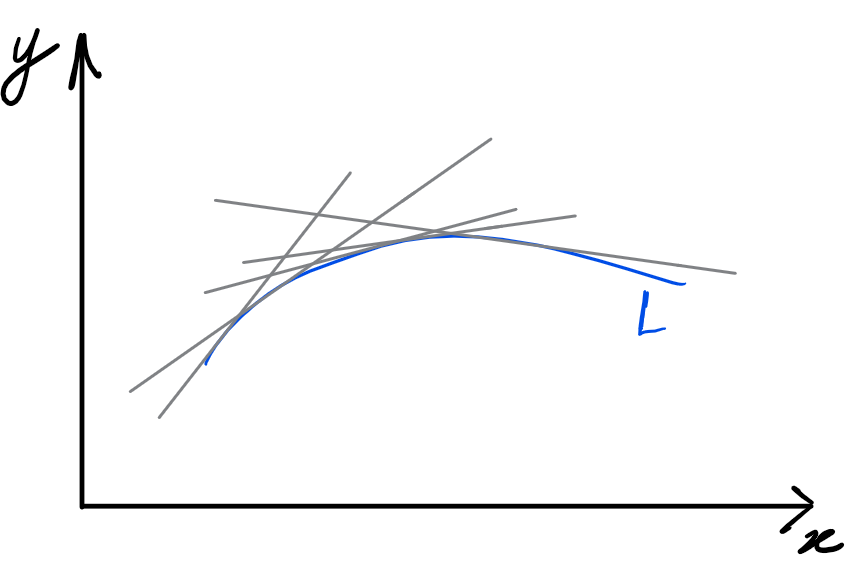
\includegraphics[width=50mm]{pictures/2_6_1.png}
            \caption{}
        }
    \end{figure}
\end{Note}

\begin{Note}[О геометрическом смысле ДУ Клеро]
    Ищем кривую $L$, касательные к которой обладают некоторым свойством. Рисунок для условия в конце.

    Уравнение касательной к $L$ в точке $(x,\;y)\in L$\\    
    \[
        Y-y = y'\,(X-x) = y'\,X - x\,y'
    \]
    Уравнение относительно $Y$ в общем виде
    \[
        Y=k\,X+b, \quad \text{где} \quad k=y', \quad b = y - x\,y'
    \]
    Объявим свойство касасательной как $b=\varphi(k)$. Тогда
    \begin{align*}
        y - x\,y' &= \varphi(y')\\
        y &= x\,y' + \varphi(y')
    \end{align*}
    Таким образом, мы получили уравнение Клеро.
    \begin{figure}[bh]
        \noindent\centering{
            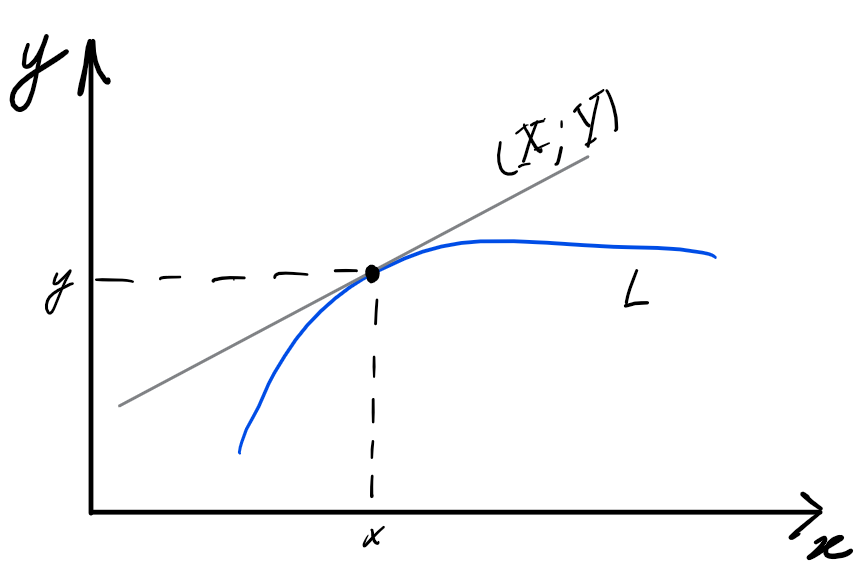
\includegraphics[width=75mm]{pictures/2_6_2.png}
            \caption{}
        }
    \end{figure}
\end{Note}

\begin{Def}
    Пусть есть функции
    \[
        (\varphi(t),\; \psi(t)) \in C'(I) \quad \varphi(t)\; \cancel{\equiv}\; t \text{ (функция нелинейна)}
    \]
    Тогда уравнение вида 
    \[
        y=x\,\varphi(y')+\psi(y')
    \] 
    называют ДУ Лагранжа.\\  
    \textcolor{cyan}{Замечание 1}. Уравнение похоже на Клеро, но тут кривая связана с нормалями.\\
    \textcolor{cyan}{Замечание 2}. \textcolor{red}{Уравнение Лагранжа общий случай уравнения Клеро.}
\end{Def}

\begin{Note}[Как решать]
    Дано
    \[
        y=x\,\varphi(y')+\psi(y')
    \]
    Решение.\\
    Введём следующую параметризацию
    \[
        \begin{cases}
            x = x(t)\\
            y = y(t)
        \end{cases}
    \]
    Тогда формуле параметрически заданной функции получаем
    \[
        y'_x=\frac{y'_t}{x'_t}=t \qquad \Rightarrow \qquad y'_t=t\,x'_t
    \]
    Так как $y'_x$ и $y'$ одно и тоже, получаем из условия
    \[
        y = x\,\varphi(t) + \psi(t)
    \]
    Продиференцируем по $t$ Получим
    \[
        y'_t = x'_t\,\varphi + x\,\varphi'_t + \psi'_t
    \]
    Помним, что $y'_t = t \, x_t'$. С учётом этого уравнение выше приобретает вид
    \begin{align*}
        x'_t\,\varphi + x\,\varphi'_t + \psi'_t = t \, x_t'\\
        x'_t\,(\varphi - t) + x\,\varphi'_t = -\psi'_t
    \end{align*}
    Таким образом получили линейное ДУ 1-го порядка в приведённой форме. Решение (через метод Лагранжа)
    \begin{align*}
        x'_t + \frac{\varphi\,'_t}{\varphi-t}\,x &= \frac{\psi'_t}{\varphi-t}\\
        x_0' + \frac{\varphi'_t}{\varphi-t}\,x_0 &= 0\\
        x_0' = \frac{\varphi'_t}{t - \varphi}\,x_0\\
        \frac{dx_0}{x_0} = \frac{\varphi'_t\, dt}{t - \varphi}
    \end{align*}
    Интегрируем и получаем решение для однородного ДУ затем находим ответ для неодродного уравнения ($x_1$). Таким образом мы нашли 
    \[
        x=x_1(t)+C\,x_0(t)
    \]
    Подставляем значение $x$ в $y'_t=t\,x'_t$ или $y = x\,\varphi(t) + \psi(t)$ \textcolor{red}{(оба варинта справедливы?)}. Получаем окончательный ответ.\\
    Таким образом, общий интеграл ДУ Лагранжа
    \[
        \begin{cases}
            x=x_1(t)+C\,x_0(t)\\
            y=y_1(t)+C\,y_0(t)
        \end{cases}
    \]
    Замечание. Нужно проверить\\
    \[
        \frac{y'_t}{x'_t}=t
    \]
    особое решение, когда $\varphi(t)-t=0$\\
\end{Note}



  %10  %OK  Q
    \author{Tkachuk Andrei}

\section{Диференциальные уравнения высшего порядка уравнения высшего порядка, доспукающие понижения порядка}

\begin{Def}
    ДУ $n$-го порядка это уравнение вида 
    \[
        F(x, y, y', y'', \dots, y^{(n)}) = 0
    \]
    решение которого является функцией $y = y(x), \; x \in I$, которая $n$ раз диференцируема на $I$ и справедливо
    \[
        F(x, y, y'(x), y''(x), \dots, y^{(n)}(x)) = 0
    \]
\end{Def}

\begin{Def}
    Если 
    \[
        y^{(n)} = F(x, y, y', y'', \dots, y^{(n - 1)})
    \] 
    то оно называется диферециалное уравнение $n$-го порядка рзрешённого относительно старшей производной
\end{Def}

\begin{Example}[Как можно описать множество решений]
    Дано
    \[
        y^{(n)} = f(x), \; f(x) \in C(I), \text{ где I --- интервал}
    \]
    Для краткости запишем через эквивалентность
    \begin{align*}
        y^{(n)}(x) &\equiv f(x)\\
        (y^{(n-1)}(x))' & \equiv f(x) &\Leftrightarrow& &y^{(n-1)}(x) &= F_1(x) + C_1\\
        (y^{(n-2)}(x))'' & \equiv f(x) &\Leftrightarrow& &y^{(n-2)}(x) &= F_2(x) + C_1 \, x + C_2
    \end{align*}
    Из этого следует
    \begin{align*} 
        y^{(n-3)} &= F_3(x) + \frac{C_1}{2} \, x^2 + C_2 \, x + C_3\\
        &\dots\\
        y &= F_n(x) + \frac{C_1}{(n+1)!}\,x^{n - 1} + \dots + C_{n - 1}\,x + C_n\\
        y &= F_n(x) + C'_1 \, x^{n - 1} + \dots + C'_{n - 1}\,x + C'_n
    \end{align*}
    где
    \[
        F_n(x) = \underbrace{\int dx \int dx \dots \int f(x)dx}_{n \text{ раз}}
    \]
    Замечание. В последней строке сделана замена вида: $C'_1 = \frac{C_1}{(n+1)!} \; \dots \; C'_n = C_n$.\\
\end{Example}

\begin{Def}[Общее решение]
    Пусть $y^{(n)} = f(x, y, y', \dots, y^{n-1})$ --- ДУ $n$-го порядка.\\
    Тогда функция 
    \[
        y = \varphi(x, C_1, \dots, C_n)
    \]
    называется общим решением этого ДУ если
    \begin{enumerate}
        \item $\forall C_1, \dots, C_n \; y = \varphi(x, C_1, \dots, C_n)$ является решением как функция от $x$
        \item Для любого решения $y = \varphi^*(x)$ найдётся такой набор $C^*_1, \dots, C^*_n \in \bb{R},\; \forall x \in I$, что $\varphi^*(x) = \varphi(x, C^*_1, \dots, C^*_n)$. То есть общее решение учитывает все наборы констант (все варианты решения)
    \end{enumerate}
\end{Def}

\begin{Def}[Общий интеграл]
    Если общее решение задано неявной функцией
    \[
        \varPhi(x, y, C_1, \dots, C_n) = 0
    \]
    то это общий интеграл
\end{Def}

\begin{Def}[Задача Коши для ДУ $n$-го порядка]
    Она описывается следующим образом
    \[
        \begin{cases}
            y^{(n)} = f(x, y, y', \dots, y^{(n-1)})\\
            y|_{x = x_0} = y_0, \; y'|_{x = x_0} = y'_0, \; \dots, \; y^{(n-1)}|_{x = x_0} = y^{n-1}_0
        \end{cases}
    \]
    где функция $f(x, y, y', \dots, y^{(n-1)})$ определена в области $D \subset \bb{R}^{n+1}$,\\
    а $M_0(x_0, y_0, y'_0, \dots, y^{n-1}_0)$ --- внутренняя точка области $D$
\end{Def}

\begin{Th}[Сущ. и ед. задачи Коши для ДУ n-го порядка]
    Пусть функция $f(x, y, y', \dots, y^{(n - 1)})$ определена в области $D \in \bb{R}^{n+1}$ и
    \[
        f(M), \; \frac{\delta f(M)}{\delta y}, \; \frac{\delta f(M)}{\delta y'}, \; \dots, \; \frac{\delta f(M)}{\delta y^{(n-1)}}
    \]
    непреывны в некоторой окрестности $U(M_0) \subset D$, где $M_0(x_0,\; y_0,\; \dots,\; y_0^{(n-1)})$\\
    
    Тогда $\exists \delta > 0$ и существует единственная функция $y = y(x), \; x \in U_\delta(x_0)$, которая является решением задачи Коши
    \[
        \begin{cases}
            y^{(n)} = f(x, y, y', \dots, y^{(n-1)})\\
            y|_{x = x_0} = y_0, \; y'|_{x = x_0} = y'_0, \; \dots, \;   y^{(n-1)}|_{x = x_0} = y^{n-1}_0
        \end{cases}
    \] 
\end{Th}

\begin{Proof}
    Принимаем без доказательств.\\
    \textcolor{cyan}{Примечание.} Доказательсво аналогично случаю для одной переменной.
\end{Proof}

\begin{Note}[О ДУ допускающих понижение порядка]
    Рассмотрим ДУ вида $F(x, y', \dots, y^{(n)}) = 0$, т.е. не содержащих в явном виде $y$.\\
    Для них спаведлива следующая замена:
    \[
        z = z(x) = y'(x), \; z'(x) = y''(x),\; \dots, \; z^{(n - 1)}(x) = y^{(n)}(x)
    \]
    Тогда
    \begin{align*}
        \begin{cases}   
            F(x, z, \dots, z^{(n-1)}) = 0\\
            z = y'
        \end{cases}\\
        \text{Таким образом, общее решение}\\
        y' = z = z(x, C_1, \dots, C_{n-1})\\
    \end{align*}
    Ответ
    \[
        y = \int z(x, C_1, \dots, C_{n-1})\,dx + C_n
    \]
\end{Note}

\begin{Example}
    Дано
    \[
        x^2\,y'' - (y')^2 = 0
    \]
    Решение.\\
    Заменияем $z = y', \; z' = y''$. Получаем
    \begin{gather*}
        x^2 \, z' - z^2 = 0\\
        \frac{dz}{z^2} = \frac{dx}{x^2}\\
        \int \frac{dz}{z^2} = \int \frac{dx}{x^2}\\
        - \frac{1}{z} = - \frac{1}{x} - C_1\\
        z = \frac{x}{C_1 \, x + 1}\\
        y' = \frac{x}{C_1 \, x + 1}\\
        y = \int \frac{x}{C_1 \, x + 1}
    \end{gather*}
    Таким образом получаем
    \begin{enumerate}
        \item $C_1 = 0 \Rightarrow y = \frac{x^2}{C_2}$
        \item Для $C_1 \neq 0$ получим
        \begin{align*}
            y &= \frac{1}{C_1} \, \int \frac{(C_1\,x + 1) - 1}{C_1\,x + 1} \, dx + C_2\\
            y &= \frac{x}{C_1} - \frac{1}{C_1^2}\,ln(|C_1\,x + 1|)  + C_2
        \end{align*}
        \item Частный случай $z = 0, \; y' = 0 \Rightarrow y = C_2$
    \end{enumerate}
\end{Example}

\begin{Note}
    Рассмотрим ДУ вида $F(x, y^{(k)}, \dots, y^{(n)}) = 0$, т.е. не содержащие в явном виде $y, y', \dots, y^{(k - 1)}, \; k \geqslant 2$s.\\
    В данном случае всё аналогично предыдущему замечанию
    \begin{gather*}
        z = y^{(k)}, z' = y^{(k + 1)}, \dots, z^{(n-k)} = y^{(n)}\\
        \begin{cases}   
            F(x,z, \dots, z^{(n-k)}) = 0\\
            z = y^{(k)}
        \end{cases}\\
        \text{Таким образом, общее решение для } z\\
        z = z(x, C_1, \dots, C_{n-k})\\
        F_k^{(k)} = z(x, C_1, \dots, C_{n-k})\\
        y^{(k)} = F_k^{(k)}\\
        y = F_k(x, C_1, \dots, C_{n-k}) + C_{n-k+1}\,x^{k-1} + \dots + C_n
    \end{gather*}
\end{Note}

\begin{Example}
    Дано
    \[
        x \, y''' - y'' = 0 \Rightarrow k = 2
    \]
    Решение
    \begin{gather*}
        \text{Пусть } z = y'', \; z' = y''' \text{ тогда}\\
        x \, z' - z = 0\\
        \int \frac{dz}{z} = \int \frac{dx}{x} + ln|C_1|\\
        z = C_1\,x
        \text{Делаем обратную замену}\\
        y'' = C_1\,x\\
        y' = \frac{C_1 \, x^2}{2} + C_2\\
        y = \underbrace{\frac{C_1 \, x^3}{6}}_{F_2(x, C_1)} + \underbrace{C_2\,x + C_3}_{\text{многочлен ст. } k - 1}
    \end{gather*}
    По факту мы рассмотрели следующее уравнение в поле
    \[
        y''' = \frac{y''}{x}, \; D \in \bb{R}^4 \setminus \{x=0\}
    \]
    Замечание. Частный случай ($z = 0$) входит в общее решение. Таким образом, решение выше полное.
\end{Example}

\begin{Note}
    Рассмотрим ДУ вида $F(y, y', \dots, y^{(n)}) = 0$ т.е. не содержащее $x$ в явном виде.\\
    Аналогично делаем замену
    \begin{align*}
        y' &= p(y)\\
        \text{Отметим } y'_x(x) &= p(y(x)) \text{ --- сложная функция. Значит}\\
        y''&=  p'\,p\\
        y''' &= (p'' \, p + (p')^2)\,p = f_2(p, p', p'')\\
        &\dots\\
        y^{(k + 1)} &= f_k(p, p', \dots, p^{(k)})
    \end{align*}
    Таким образом получаем следующую систему
    \[
        \begin{cases}
            F(y,\; p,\; p'\,p,\; f_2(p,\; p',\; p''),\; \dots,\; f_k(p,\; p',\; \dots,\; p^{(k)})) = 0\\
            y' = p
        \end{cases}
    \]
    Следователно общее решение относительно $p$
    \[
        p = p(y, C_1, \dots, C_{n-1})
    \]
    Зная, что $y' = p$ получаем
    \[
        \frac{dy}{p(y, C_1, \dots, C_{n-1})} = dx
    \]
    Таким образом решение относительно $x$ следующее
    \[
        x = \int \frac{dy}{p(y, C_1, \dots, C_{n-1})} + C_n
    \]
\end{Note}

\begin{Example}
    Дано
    \[
        y'' = 2\,y\,y'
    \]
    Решение
    \begin{align*}
        y' &= p(y)\\
        y'' &= p'\,p\\
        p'\,p &= 2\,y\,p\\
        p(p' - 2\,y) &= 0
    \end{align*}
    Получаем два случая\\
    Первый:
    \[
        p = 0 \Rightarrow \; y' = 0, \; y = C_1 
    \]
    Второй:
    \begin{align*}
        p'- 2\,y &= 0\\
        p' &= 2\,y\\
        dp &= 2\,y\,dy\\
        \int dp &= \int 2\,y\,dy\\
        p = y' &= y^2 + C_1\\
        \frac{dy}{dx} &= y^2 + C_1\\
        \int dx  &= \int \frac{dy}{y^2 + C_1}\\
        x + C_2 &= \int \frac{dy}{y^2 + C_1}\\
    \end{align*}
    При вычислении интеграла рассмотрим три случая
    \begin{enumerate}
    \item $C_1 = 0$  
    \begin{align*}
        -\frac{1}{y} &= x + C_2\\
        y &= -\frac{1}{x + C_2}
    \end{align*} 
                  
     \item $C_1 > 0$
     \begin{align*}
        x + C_2 &= \frac{1}{\sqrt{C_1}}\, arctg\left(\frac{y}{\sqrt{C_1}}\right)\\
        y &= \sqrt{C_1} \, tg((x + C_2)\, \sqrt{C_1})
     \end{align*}   
                
     \item $C_1 < 0, \; C_1 = -|C_1|$
     \begin{align*} 
        x + C_2 &= \frac{1}{2\,\sqrt{|C_1|}}\, ln\left|\frac{y-\sqrt{|C_1|}}{y+\sqrt{|C_1|}}\right|
     \end{align*}
    \end{enumerate}
\end{Example}  %11  %OK
    \section{Линейные ДУ n-го порядка}

\begin{Def}
    Пусть сущ. функции $p_1(x),\, \dots,\, p_n(x),\, f(x) \in C_{(a;\,b)}$. Тогда ДУ вида
    \[
        y^{(n)} + p_1(x)\,y^{(n-1)} + \dots + p_n(x)\,y = f(x)
    \]
    называется лининейным ДУ n-го порядка с коэфициентами $p_1(x),\; \dots,\; p_n(x)$ и правой частью $f(x)$
\end{Def}

\begin{Th}[Cущ. и ед. задачи Коши для ЛДУ n-го порядка]
    Пусть $p_1(x),\, \dots,\, p_n(x), \,f(x) \in C_{(a;\;b)}$.\\ 
    Тогда $\forall x_0 \in (a;\,b)$, $\forall y_0,\, y_0',\, \dots,\, y_0^{(n-1)} \in \bb{R}$ задача Коши
    \[
        \begin{cases}
            y^{(n)}+p_1(x)y^{(n-1)}+\dots+p_n(x)y=f(x)\\
            y|_{x=x_0}=y_0, \dots , y^{(n-1)}|_{x=x_0}=y_0^{(n-1)}
        \end{cases}
    \]
    имеет единственное решение $y=y(x)$, $x\in (a,\,b)$ определённое на всём интервале $(a;\,b)$.
\end{Th}

\begin{Proof}
    Принимаем без доказательств
    
\end{Proof}

Для более компактной записи введём следующее определение
\begin{Def}[Линейный диференциальный оператор]
    Перед тем как непосредственно вводить определение рассмотрим два случая.
    \begin{enumerate}
        \item Рассмотрим оператор диференцирования: $\frac{d}{dx}$, тогда его действие будет выглядеть так 
        \[
            \frac{d}{dx}\,f(x)=\frac{df(x)}{dx}=f'(x)
        \]
        Данный оператор линейный, так как
        \begin{enumerate}
            \item $(v+u)'=v'+u'$
            \item $(cu)'=c\,u'$
        \end{enumerate}
        (Примечание. признак линейности см. во 2м сем.)
        
        \item Для другого оператора $\frac{d^k}{dx^k}$ действие будет выглядеть \[
            \frac{d^k}{dx^k}f(x)=\frac{d^kf(x)}{dx^k}=f^(k)(x)
        \]
        Сам оператор также является линейным
    \end{enumerate}
    Таким образом, очевидно, что в общем случае можно определить оператор
    \[
        L=\frac{d^n}{dx^n}+p_1(x)\frac{d^{n-1}}{dx^{n-1}}+\dots +p_{n-1}(x)\frac{d}{dx}+p_n(x)E
    \] 
    это линейный диференциальный оператор $n$-го порядка, где
    \[
        Ef(x)=f(x) \text{ E --- единичный оператор}
    \]
    
    Его действие на n раз диф. ф-ю $f(x)$
    \begin{align*}
        L&=\frac{d^nf(x)}{dx^n} + p_1(x)\,\frac{d^{n-1}f(x)}{dx^{n-1}}+ \dots +p_{n-1}(x)\,\frac{df(x)}{dx}+p_n(x)\,f(x)\\
        L(y)&=y^{(n)}+p_1(x)\,y^{(n-1)}+p_{n-1}\,(x)y'+p_n(x)\,y    
    \end{align*}
\end{Def}



\begin{Note}
    Теперь ЛДУ n-го порядка можно описать так 
    \[
        L(y)=f(x)
    \]
\end{Note}

\begin{Note}[Линейность оператора $L$].\\
    Пусть 
    \[
        L=\frac{d^n}{dx^n}+p_1(x)\,\frac{d^{n-1}}{dx^{n-1}}+ \dots +p_{n-1}(x)\,\frac{d}{dx}+p_n(x)\,E
    \]
    Тогда
    \begin{enumerate}
        \item $L(\varphi_1(x)+\varphi_2(x))=L(\varphi_1(x))+L(\varphi_2(x))$
        \item $L(C\,\varphi(x))=C\,L(\varphi(x))$
        \item $L(C_1 \, \varphi_1(x)+C_2 \, \varphi_2(x) + \dots + C_n\varphi_n(x))=C_1\, L(\varphi_1(x))+C_2 \, L(\varphi_2(x)) + \dots + C_n \, L(\varphi_n(x))$
    \end{enumerate}
 \end{Note}

\begin{Proof}
     \begin{enumerate}
        \item Рассмотрим следующие тривиальные выражения
        \begin{align*}
        \varphi_1(x)+\varphi_2(x) &=\varphi_1(x)+\varphi_2(x)\\
        (\varphi_1(x)+\varphi_2(x))' &=\varphi'_1(x)+\varphi'_2(x)\\
        (\varphi_1(x)+\varphi_2(x))'' &=\varphi''_1(x)+\varphi''_2(x)\\
        &\dots\\
        (\varphi_1(x)+\varphi_2(x))^{(n)} &=\varphi^{(n)}_1(x)+\varphi^{(n)}_2(x)
        \end{align*}
        Каждую из строк соответственно умножим на $p_n,\; p_{n-1},\; \dots, \; p_1,\; 1$.
        Затем сложим все уравнения. И нетрудно заметить, что таким образом получаем
        \[
            L(\varphi_1(x)+\varphi_2(x))=L(\varphi_1(x))+L(\varphi_2(x))
        \]
        
        \item аналогично доказывается (рассмотрим выражения $c\,\varphi, (c\,\varphi)^{(n)}$)
        
        \item аналогично (или методом мат. индукции по $k$)
    \end{enumerate}
\end{Proof}

\begin{Def}
    \begin{align}
        L(y)&=y^{(n)}+p_1(x)\,y^{(n-1)}+p_{n-1}(x)\,y'+\dots+p_n(x)\,y=f(x)\\
        L(y)&=y^{(n)}+p_1(x)\,y^{(n-1)}+p_{n-1}(x)\,y'+\dots+p_n(x)\,y=0
    \end{align}
    ДУ (2) называют линейным однородным ДУ, а (1) лин. неоднородным ДУ\\
    В краткой форме соответствует
    \begin{align*}
        L(y)&=f(x)\\
        L(y)&=0
    \end{align*}
\end{Def}

\begin{Note}.\\
    ЛОДУ --- линейное однородное диференциальное уравнение\\
    ЛНДУ --- линейное неоднородное диференциальное уравнение
\end{Note}

\begin{Th}[О линейности мн-ва решений ЛОДУ]
    Пусть функции $p_1(x),\, \dots,\, p_n(x),\, f(x) \in C_{(a;\,b)}$ и $L(y)=y^{(n)}+p_1(x)\,y^{(n-1)}+p_{n-1}\,(x)y'+ \dots + p_n(x)\,y$.
    Тогда ЛОДУ $L(y) = 0$ имеет множество решений удвлетворяющие следующему свойству линейности.\\
    Если $\varphi_1(x),\, \dots,\, \varphi_k(x)$ решение $L(y)=0$, то\\
    $\forall C_1,\, \dots,\, C_k \in \bb{R}$ функция 
    \[
        y = C_1\,\varphi_1(x) + \dots + C_k\,\varphi_k(x)  
    \]
    является решением $L(y)=0$\\
    
    \textcolor{cyan}{Замечание}. Количество решений произвольно и не обязательно равно $n$.
\end{Th}

\begin{Proof}.\\
    Дано 
    \[
        L(\varphi_1(x))\equiv 0,\; \dots,\; L(\varphi_k(x))\equiv 0
    \]
    Тогда для $\forall C_1,\, \dots,\, C_k$ и свойствам из замечания 2 получаем
    \[
        L(C_1\varphi_1(x) + \dots + C_n\,\varphi_n(x)) = C_1\,L(\phi_1(x)) + \dots + C_n\,L(\varphi_n(x))\equiv 0
    \]
    Следовательно $y=C_1\,\varphi_1(x)+ \dots + C_k\,\varphi_k(x)$ является решением $L(y)=0$
    
\end{Proof}
  %12  %OK
    \section{Фундаментальная система решений ЛОДУ}

\begin{Def}[Линейно зависимая система функций]
    Система функций $\{\varphi_1(x),\; \dots, \;\varphi_k(x)\}$ определённая на $(a;\,b)$ называется линейно зависимой
    \begin{align*}
        \Leftrightarrow\\
        &\exists \alpha_1, \dots, \alpha_k \in \bb{R}& &\alpha^2_1 + \dots + \alpha^2_k \neq 0\\
        &\forall x \in(a;\,b)& &\alpha_1\,\varphi_1(x)+\dots+\alpha_k\,\varphi_k(x)=0    
    \end{align*}
    \textcolor{cyan}{Примечание.} Говорят: лин. зав. на интервале $(a;\,b)$. Важно отметить, что мы рассматриваем систему на интервале.
\end{Def}

\begin{Example}
    Дана линейно зависимая система на $\bb{R}$ 
    \[
        \{x,\; x+1,\; x-1\}
    \]
    Требуется найти набор коэфициентов.\\ 
    Решение
    \begin{align*}
        \alpha\,x+ \beta\,(x+1)+\gamma\,(x-1) &\equiv 0\\
        (\alpha + \beta +\gamma )\,x + \beta - \gamma &\equiv 0
    \end{align*}
    Очевидно, что решение будет тогда, когда выполнена следующая система
    \[
    \begin{cases}
        \alpha + \beta+\gamma=0\\
        \beta - \gamma = 0
    \end{cases}
    \]
    Таким образом, решение
    \[    
    \begin{cases}
        \alpha=-2\beta\\
        \beta=\beta\\
        \gamma = \beta
    \end{cases}
    \]
    Ответом может быть, например, частный случай при $\beta =1$ тогда $\alpha=-2,\; \beta =1, \; \gamma=1$\\
    $-2x+(x+1)+(x-1)\equiv 0$ --- система линейно зависима на $\bb{R}$
\end{Example}

\begin{Def}[Линейно независимая система функций]
    Система функций  $\{\varphi_1(x),\; \dots,\; \varphi_k(x)\}$ опр-на на $(a;b)$ называется линейно независимой на $(a;b)$\\
    Или
    \[
        \{ \phi_1(x),\dots,\phi_k(x)\} \text{ не явл. лин. зав. на } (a;b)
    \]
    Или
    \begin{align*}
        &\forall x \in(a;\,b) \quad \alpha_1\,\phi_1(x) + \dots + \alpha_k\,\phi_k(x)=0\\
        &\text{Где }ы \alpha_1 = \dots = \alpha_k = 0\\
    \end{align*}
\end{Def}

\begin{Def}[Фундаментальная система решений ЛОДУ].\\
    Пусть 
    \[
        p_1(x),\dots,p_n(x)\in C_{(a;b)}
    \]
    ЛОДУ 
    \[
        L(y)=y^{(n)} + p_1(x)\,y^{(n-1)} + p_{n-1}(x)\,y' + \dots + p_n(x)\,y=0
    \]
    Система функций  $\{ \varphi_1(x),\, \dots,\, \varphi_k(x)\}$ определена на $(a;\,b)$ 
    называется фундаментальной системой решений ЛОДУ $L(y)=0$\\
    $\Leftrightarrow$
    \begin{enumerate}
        \item $L(\varphi_1(x))\equiv 0$,\dots,$L(\varphi_n(x))\equiv 0$\\
        Где $x \in (a;\,b) $ и $ \varphi_1,\, \dots,\, \varphi_n$ --- решения ЛОДУ
        
        \item число функций равно $n = \{\text{порядок ЛОДУ}\}$
        
        \item $\{ \varphi_1(x),\, \dots,\, \varphi_n(x)\}$ - лин. незав. система на $(a;\,b)$
    \end{enumerate}
\end{Def}

\begin{Def}
    Пусть функции $ \varphi_1(x),\, \dots,\, \varphi_n(x)$ n раз дифф-мая функция на $(a;\,b)$\\
    Тогда функциональный определитель
    \[
        W(x)=W(\varphi_1,\;\dots,\;\varphi_n) = 
        \begin{vmatrix} 
            \varphi_1 &\dots & \varphi_n\\ 
            \vdots& \dots &\vdots\\
            \varphi_1^{(n-1)} & \dots &\varphi_n^{(n-1)} 
        \end{vmatrix}
    \]
    называется определителем Вронского или Вронскиан для системы функций $\{\varphi_1(x),\;\dots,\;\varphi_n(x)\}$
\end{Def}

\begin{Th}
    В условиях определения 4, если система функций
    \[
        \{\varphi_1(x),\; \dots,\; \varphi_n(x)\} \quad \text{линейно зависима на } (a;\;b)
    \]
    то
    \[
        \forall \alpha \in (a;\;b), \quad W(x) = W(\varphi_1,\;\dots,\;\varphi_n)=0
    \]
    
    
\end{Th}

\begin{Proof}
    $\exists \; \alpha_1,\;\dots,\;\alpha_n$, причём $\alpha_1^2 + \dots + \alpha^2_n \neq 0$ а также
    \[
        \forall x \in(a;\,b) \quad \alpha_1\,\phi_1(x)+\dots+\alpha_k\,\phi_k(x)=0
    \]
    Зафиксируем один из коэфициентов и будем считать, что $\alpha_1 \neq 0$ (в случаее, если другой коэфициент не равен нулю, то его можно поменять местами с $\alpha_1$)
    \begin{gather*}
        W = 
        \begin{pmatrix} 
            \varphi_1 & \dots &\varphi_n \\ 
            \vdots & \dots & \vdots\\ 
            \varphi_1^{(n-1)} & \dots & \varphi_n^{(n-1)} 
        \end{pmatrix}
        = \frac{1}{\alpha_1}
        \begin{pmatrix}
            \alpha_1\,\varphi_1 & \dots & \varphi_n \\ 
            \dots & \dots & \dots\\ 
            \alpha_1\,\varphi_1^{(n-1)} & \dots & \varphi_n^{(n-1)} 
        \end{pmatrix} 
        =\\
        = [\text{ Добавляем к первому столбцу столбцы умноженные на }\alpha_2,\; \dots,\; \alpha_n \;] =\\
        =\frac{1}{\alpha_1}
        \begin{pmatrix} 
            \alpha_1\,\phi_1 + \dots + \alpha_n\,\phi_n & \varphi_2 & \dots &\varphi_n \\ 
            \dots & \dots & \dots & \dots\\
            \alpha_1\,\phi_1^{(n-1)}+\dots+\alpha_n\,\phi_n^{(n-1)} & \varphi_2^{(n - 1)} &\dots &\phi_n^{(n-1)} 
        \end{pmatrix} 
        =\\
        =\frac{1}{\alpha_1}
        \begin{pmatrix} 
            \alpha_1\,\phi_1 + \dots + \alpha_n\,\phi_n & \varphi_2 & \dots &\varphi_n \\ 
            \dots & \dots & \dots & \dots\\
            (\alpha_1\,\phi_1 + \dots + \alpha_n\,\phi_n)^{(n-1)} & \varphi_2^{(n - 1)} &\dots &\phi_n^{(n-1)} 
        \end{pmatrix} 
        =\\
        =\frac{1}{\alpha_1}
        \begin{pmatrix} 
            0 & \varphi_2 & \dots & \varphi_n \\
            0 & \varphi'_2 & \dots & \varphi'_n \\ 
            \dots & \dots & \dots & \dots \\ 
            0 & \phi_2^{(n-1)} & \dots & \varphi_n^{(n-1)} 
        \end{pmatrix}
        = 0 \qquad \forall x \in (a;\,b)
    \end{gather*}
\end{Proof}

\begin{Note}
    Пусть $\{\varphi_1(x),\; \dots,\; \varphi_n(x)\}$ $n$ раз диференцируемая система функций на $(a;\;b)$, $W(x) = W(\varphi_1(x),\; \dots,\; \varphi_n(x))$ --- вронскиан системы $\{\varphi_1(x),\; \dots,\; \varphi_n(x)\}$\\
    
    Тогда если $\exists x_0 \in (a;\;b) \; W(x_0) \neq 0$ то система $\{\varphi_1(x),\; \dots,\; \varphi_n(x)\}$ линейна независима на $(a;\;b)$
\end{Note}

\begin{Proof}
    Доказательство от противного.\\
    Пусть $W(x_0) \neq 0$ и система линейно зависима на промежутке. Следовательно теореме выше получаем, что вронскиан равен нулю $\forall x\in(a\;b)$, следовательно, в частности, $W(x_0) = 0$, что противоречит первоначальному условию $W(x_0) \neq 0$. Таким образом, получаем противоречие и следовательно система линейно независима на интервале. 
\end{Proof}\\

Вспомним теорему 1 из предыдущего параграфа (она нужна для доказательства следующей теоремы)
\begin{Th}
    Пусть $p_1(x),\, \dots,\, p_n(x), \,f(x) \in C_{(a;\;b)}$.\\ 
    Тогда $\forall x_0 \in (a;\,b)$, $\forall y_0,\, y_0',\, \dots,\, y_0^{(n-1)} \in \bb{R}$ задача Коши
    \[
        \begin{cases}
            L(y) = y^{(n)}+p_1(x)\,y^{(n-1)}+\dots+p_n(x)\,y=f(x)\\
            y|_{x=x_0}=y_0, \dots , y^{(n-1)}|_{x=x_0}=y_0^{(n-1)}
        \end{cases}
    \]
    имеет единственное решение $y=y(x)$, $x\in (a,\,b)$ определённое на всём интервале $(a;\,b)$.
\end{Th}

\begin{Th}
    Пусть в условиях теоремы выше функции $\{\varphi_1(x),\; \dots,\; \varphi_n(x)\}$ является решением ЛОДУ $L(y) = 0$ и $\exists x_0 \in (a;\, b),\; W(x_0) = 0$.\\
    
    Тогда $\{\varphi_1(x),\; \dots,\; \varphi_n(x)\}$ линейно зависима на всём промежутке и (по т. 1) $\forall x \in (a,\;b)\; W(x) = 0$
\end{Th}

\begin{Proof}
    Рассмотрим алгебраическую систему уравнений относительно $C_1, \dots, C_n$, получим
    \[
        \begin{cases}   
            C_1\,\varphi_1(x_0) + \dots + C_n\,\varphi_n(x_0) = 0\\
            C_1\,\varphi_1'(x_0) + \dots + C_n\,\varphi_n'(x_0) = 0\\
            \vdots\\
            C_1\,\varphi_1^{(n - 1)}(x_0) + \dots + C_n\,\varphi_n^{(n - 1)}(x_0) = 0
        \end{cases}
    \]
    $n$ уравнений относительно $n$ переменных $C_1,\dots,C_n$ и $\Delta = W(x_0) = 0$. Значит ранг матрицы меньше $n$, следовательно существует бесконечное множество решений (см. 2 сем.), то есть
    \[
        \exists (C_1^*,\; \dots,\; C_n^*) \neq (0,\; \dots,\; 0)
    \]
    Рассмотрим
    \[
       \varphi^*(x) = C_1^*\,\varphi_1(x_0) + \dots + C_n^*\,\varphi_n(x_0)
    \]
    $\varphi^*(x)$ --- является решением задачи Коши
    \[
        \begin{cases}
            L(y) = 0\\
            y|_{x=x_0}=0, \dots , y^{(n-1)}|_{x=x_0}=0
        \end{cases}
    \]
    То есть
    \[
        \varphi^*(x_0) = 0,\; (\varphi^*)'(x_0) = 0,\; \dots,\; (\varphi^*)^{(n-1)}(x_0) = 0
    \]
    Очевидно, что для $y \equiv 0$, также является решением тойже задачи Коши на интервале. Примечание $ L(y) = y^{(n)}+p_1(x)\,y^{(n-1)}+\dots+p_n(x)\,y$. Из всего этого следует
    \[
        \varphi^*(x_0) \equiv 0 \quad \Rightarrow \quad \forall x \in (a;\;b) \quad C_1^*\,\varphi_1(x) + \dots + C_n^*\,\varphi_n(x) = 0
    \]
    где $(C_1^*,\; \dots,\; C_n^*) \neq (0,\; \dots,\; 0)$.\\
    Значит по определению линейно зависимой системы, получаем что система $\{\varphi_1(x),\; \dots,\; \varphi_n(x)\}$ линейно зависима на $(a;\;b)$
\end{Proof}

\begin{Th}[О существовании ФСР ЛОДУ $n$-го порядка]
    Пусть функции $p_1(x),\; \dots,\; p_n(x) \in C_{(a;\;b)}$, тогда существует набор функций $\{\varphi_1(x),\; \dots,\; \varphi_n(x)\}$ являющийся ФСР для
    \[
        L(y) = y^{(n)} + p_1(x)\,y^{(n - 1)} + \dots + p_1(x)\,y = 0
    \]
\end{Th}

\begin{Proof}
    Возьмём $x_0 \in (a;\;b)$ и рассмотрим $n$ задач Коши вида:
    \begin{align*}
        &L(y) = 0 && L(y) = 0 && \dots &&  L(y) = 0\\
        &y|_{x=x_0} = 1 && y|_{x=x_0} = 0 && \dots &&  y|_{x=x_0} = 0\\
        &y'|_{x=x_0} = 0 && y'|_{x=x_0} = 1 && \dots && \vdots \\
        &\vdots && \vdots && \dots && y^{n-2}|_{x=x_0} = 0\\
        &y^{n-1}|_{x=x_0} = 0 && y^{n-1}|_{x=x_0} = 0 && \dots && y^{n-1}|_{x=x_0} = 1\\
        & y = \varphi_1(x) && y = \varphi_2(x) && \dots && y = \varphi_n(x)\\
        & x \in(a;\,b) && x \in(a;\,b) && \dots  && x \in(a;\,b)
    \end{align*}
    \textcolor{red}{Вопросы!}\\
    Таким образом имеем следующий вронскиан
    \[
        W(x_0) = \begin{bmatrix}
            1 & 0 & \dots & 0\\
            0 & 1 & \dots & \vdots\\
            \vdots & \vdots & \ddots & 0\\
            0 & 0 & \dots & 1\\
        \end{bmatrix} = 1 \neq 0
    \]
    Из того, что определитель не равен нулю следует
    \begin{enumerate}
        \item $\varphi_1,\; \dots,\; \varphi_n$ --- решения $L(y) = 0$ на $x \in(a;\,b)$
        \item Количество решений равно порядку ДУ ($L(y) = 0$), которое равно $n$ 
        \item $\{\varphi_1,\; \dots,\; \varphi_n\}$ --- линейно независимы на $(a;\,b)$ (по следствию к теореме 1)
    \end{enumerate}
    Из этого по определению 3 следует, что $\{\varphi_1,\; \dots,\; \varphi_n\}$ --- ФСР $L(y) = 0$\\
\end{Proof}

\begin{Th}[Формула Лиувилля]
    Пусть $p_1(x),\; \dots,\; p_n(x) \in C_{(a;\;b)}$ и $\{\varphi_1(x),\; \dots,\; \varphi_n(x)\}$ --- ФСР ЛОДУ $L(y) = 0$.\\
    
    Возьмём $x_0 \in (a;\;b)$ и обозначим через $W_0 = W(x_0) \neq 0$. Тогда справедлива формула Лиувилля
    \[
        W(x) = W_0\,e^{- \int_{x_0}^x p_1(t)\,dt}
    \]
\end{Th}

\begin{Proof}
    Для наглядности рассмотрим случай $n = 2$, тогда
    \[
        L(y) = y'' + p_1(x)\,y' + p_2(x)\,y = 0
    \]
    Пусть $\{\varphi_1(x),\; \varphi_2(x)\}$ --- ФСР, то есть
    \[
        \begin{cases}
            \varphi_1'' + p_1\,\varphi_1' + p_2\,\varphi_1 = 0\\
            \varphi_2'' + p_1\,\varphi_2' + p_2\,\varphi_2 = 0
        \end{cases}
    \]
    Рассмотрим вронскиан и его производную.
    \begin{align*}
        W(x) &= \begin{cases}
           \varphi_1 & \varphi_2\\
           \varphi_1' & \varphi_2'
        \end{cases} = \varphi_1\,\varphi_2' - \varphi_2\,\varphi_1'\\
        W'(x) &= \cancel{\varphi_1'\,\varphi_2'} + \varphi_1\,\varphi_2'' - \varphi_1''\,\varphi_2 - \cancel{\varphi_1'\,\varphi_2'}
    \end{align*}
    Воспользуемся системой выше для замены $\varphi_1''$ и $\varphi_2''$. Получим.
    \begin{gather*}
        \begin{cases}
            \varphi_1'' = - p_1\,\varphi_1' - p_2\,\varphi_1\\
            \varphi_2'' = - p_1\,\varphi_2' - p_2\,\varphi_2
        \end{cases}\\
         W'(x) = \varphi_1\, (- p_1\,\varphi_2' - p_2\,\varphi_2) + \varphi_2(p_1\,\varphi_1' + p_2\,\varphi_1)\\
         W'(x) = - p_1\,(\varphi_1\,\varphi_2' - \varphi_1'\,\varphi_2) = - p_1\,W
    \end{gather*}
    Решаем тривиальное ДУ
    \[
        \frac{dW}{dx} = -p_1(x)\,W
    \]
    Очевидно
    \[
        \int_{x_0}^x ln(W) = - \int_{x_0}^x p_1(t)\,dt
    \]
    Ответ
    \[
        W(x) = W(x_0)^{- \int_{x_0}^x p_1(t)\,dt}
    \]
\end{Proof}  %13  %OK  Q
    \author{Tkachuk Andrey}

\section{Общее решение линейного ДУ n-го порядка}

\begin{Th}[Об общем решении ЛОДУ n-го порядка]
    Пусть
    \[
        p_1(x),\; \dots,\; p_n(x)\; \in C_{(a;\;b)} \text{ и } \{\varphi_1(x),\; \dots,\; \varphi_n(x)\}
    \]
    ФСР ЛОДУ
    \[
        L(y) = y^{(n)} + p_1(x)\,y^{(n-1)} + \dots + p_1\,y = 0
    \]
    Тогда функция 
    \[
        y = C_1\,\varphi_1(x) + \dots + C_n\,\varphi_n(x)
    \]
    описывает множетсво всех решений ЛОДУ $L(y) = 0$, то есть
    \begin{enumerate}
        \item $\forall\;C_1,\; \dots,\; C_n\;\in \bb{R} \qquad y = C_1\,\varphi_1 + \dots + C_n\,\varphi_n$ --- решение $L(y) = 0$ 
        \item $\forall y = \varphi^*(x)$ --- решение $L(y) = 0$. Тогда
        \begin{gather*}
            \exists \; C_1^*,\; \dots,\; C_n^*\; \in \bb{R} \quad x\in(a;\;b)\\
            \varphi^*(x) = C_1^*\,\varphi_1 + \dots + C_n^*\,\varphi_n
        \end{gather*}
    \end{enumerate}
\end{Th}

\begin{Proof}
    \begin{enumerate}
        \item Дано $L(\varphi_1) = 0,\; \dots,\; L(\varphi_n) = 0$
        \begin{gather*}
            \forall C_1,\; \dots,\; C_n \quad L(C_1\,\varphi_1 + \dots + C_n\,\varphi_n) = C_1\,\underbrace{L(\varphi_1)}_{ = 0} + \dots + C_n\,\underbrace{L(\varphi_n)}_{ = 0}\\
            \Rightarrow \; y = C_1\,\varphi_1(x) + \dots + C_n\,\varphi_n(x) \quad \text{--- решение } L(y) = 0, x \in (a;\, b)
        \end{gather*}
            
        \item Пусть $y = \varphi^*(x)$ --- решение $L(y) = 0 \quad x \in (a;\,b)$\\
        Возьмём точку $x_0 \in (a;\,b)$ и скажем, что
        \[
            y_0 = \varphi_1^*(x_0),\; \dots,\; y_0^{(n-1)} = (\varphi_n^*)^{(n-1)}(x_0)
        \]
        Тогда $y = \varphi^*(x)$ является решением задачи Коши
        \[
            \begin{cases}
                L(y) = y^{(n)}+p_1(x)\,y^{(n-1)}+\dots+p_n(x)\,y=f(x)\\
                y|_{x=x_0}=y_0, \dots , y^{(n-1)}|_{x=x_0}=y_0^{(n-1)}
            \end{cases}
        \]
        С другой строны будем искать решение этой задачи Коши в виде $y = C_1\,\varphi_1(x) + \dots + C_n\,\varphi_n(x)$\\
        тогда решение имеет вид
        \[
            \begin{cases}
                C_1\,\varphi_1(x_0) + \dots + C_n\,\varphi_n(x_0) = y_0\\
                C_1\,\varphi_1'(x_0) + \dots + C_n\,\varphi_n'(x_0) = y_0'\\
                \vdots\\
                C_1\,\varphi_1^{(n-1)}(x_0) + \dots + C_n\,\varphi_n^{(n-1)}(x_0) = y_0^{(n-1)}
            \end{cases}
        \]
        Это система $n$ алгебраических уравнений относительно $n$ переменных $C_1,\; \dots,\; C_n$, определитель которой $\Delta = W(x_0) \neq 0$, так как мы рассматриваем ФРС (система уравнений ленейно независима по определению).\\
        
        По т. Крамера следует, что существует решение и притом единственное, то есть
        \[
            \exists (C_1^*,\; \dots,\; C_n^*)
        \]
        Следовательно $y = C_1^*\,\varphi_1(x) + \dots + C_n^*\,\varphi_n(x)$ --- решение задачи Коши для $\varphi^*(x)$ по теореме о существовании и единственности задачи Коши.
    \end{enumerate}
\end{Proof}

\begin{Th}[Об общем реешении ЛНДУ n-го порядка]
    Пусть $p_1(x),\; \dots,\; p_n(x),\; f(x) \in (a;\, b)$ и $\{\varphi_1(x),\; \dots,\; \varphi_n(x)\}$ --- ФСР ЛОДУ
    \[
        L(y) = y^{(n)} + p_1(x)\,y^{(n - 1)} + \dots + p_n(x)\,y = 0 \qquad x\in (a;\,b)    
    \]
    
    Обозначим через $\psi(x)$ некоторое решение ЛНДУ $L(y) = f(x)$. Тогда общее решение ЛНДУ имеет вид
    \[
        y = \psi(x) + C_1\,\varphi_1(x) + \dots + C_n\,\varphi_n(x)
    \]
    То есть
    \begin{enumerate}
        \item $\forall \; C_1,\; \dots,\; C_n \; \in \bb{R} \quad y = \psi + C_1\,\varphi_1 + \dots + C_n\,\varphi_n$ является решением $L(y) = f(x)$
            
        \item Для любого решения $\psi^*(x)$ ЛНДУ $L(y) = f(x)$\\
        $\exists \; C_1,\; \dots,\; C_n \quad x\in(a;\,b) \quad \psi^* = \psi + C_1^*\,\varphi_1 + \dots + C_n^*\,\varphi_n$
            
    \end{enumerate}
\end{Th}

\begin{Proof}
    
    $\forall x_0 \in (a;\,b),\; \exists y_0, y_0', \dots, y_0^{(n-1)},\; \psi(x)$ --- решение здачи Коши
    \[
        \begin{cases}
            L(y) = f(x)\\
            y|_{x = x_0} = y_0,\; y'|_{x = x_0} = y_0',\; \dots,\; y^{(n-1)}|_{x = x_0} = y^{(n-1)}_0,
        \end{cases}
    \]
    По теореме о существовании и единственности задачи Коши
    \begin{enumerate}
        \item Аналогично доказательству выше имеем
        \begin{align*}
            &\forall \; C_1,\; \dots,\; C_n\\
            &L(\psi + C_1\,\varphi_1 + \dots + C_n\,\varphi_n) = \underbrace{L(\psi)}_{= f(x)} + C_1\,\underbrace{L(\varphi_1)}_{= 0} + \dots + C_n\,\underbrace{L(\varphi_n)}_{= 0} = f(x)
        \end{align*}
        
        \item $y = \psi^*(x)$ решение $L(\psi^*) = f(x)$, с другой стороны $L(\psi) = f(x)$ тоже решение (по усл.)\\
        Тогда рассмотрим следующее выражение
        \[
            L(\psi^* - \psi) = [\text{по св-ву лин. оп.}] = L(\psi^*) - L(\psi) = f(x) - f(x) = 0
        \]
        Значит $L(\psi^* - \psi)$ --- ЛОДУ. Следовательно по теореме 1 для ЛОДУ справедливо
        \[
            \exists \; C_1^*,\; \dots,\; C_n^* \quad \forall x\in(a;\,b)  \varphi^* = \psi^* - \psi = C_1^*\,\varphi_1 + \dots + C_n^*\,\varphi_n 
        \]
        Нетрудно заметить и вывести
        \[
            \psi^* = \psi + C_1^*\,\varphi_1 + \dots + C_n^*\,\varphi_n
        \]
    \end{enumerate}
\end{Proof} %14  %OK
    \author{Tkachuk Andrei}

\section{Метод вариации произвольных постоянных}

\begin{Th}
    Пусть 
    \[
        p_1(x),\; \dots,\; p_n(x),\; f(x) \in C_{(a;\,b)}
    \]
    и изветна ФСР $\{\varphi_1(x),\, \dots\,\, \varphi_n(x)\}$ ЛОДУ
    \[
        L(y) = y^{(n)} + p_1\,y^{(n-1)} + \dots + y\,p_n(x) = 0
    \]
    Ищем решение ЛНДУ $L(x) = f(x)$ в виде 
    \[
        y = C_1(x)\,\phi_1(x) + \dots + C_n(x)\,\phi_n(x)
    \]
    где функции $\{C_1(x),\, \dots,\, C_n(x)\}$ диференцируемые на $(a;\, b)$
    и $\{C'_1(x),\, \dots,\, C'_n(x)\}$ удовлетворяет следующим свойствам алгебраических уравнений
    \[
        \begin{cases}
            C'_1\,\phi'_1(x) + \dots + C'_n\,\phi'_n(x) = 0\\
            C'_1\,\phi'_1(x) + \dots + C'_n\,\phi'_n(x) = 0\\
            \vdots
            C'_1\,\phi^{(n-2)}_1(x) + \dots + C_n\,\phi^{(n-2)}_n(x) = 0\\
            C'_1\,\phi^{(n-1)}_1(x) + \dots + C_n\,\phi^{(n-1)}_n(x) = f(x)\\
        \end{cases}
    \]
    Тогда такая система имеет решения
    \begin{gather*}
        C'_1 = u_1(x),\; \dots,\; C_n = u_n(x)\\
        y = \left[\left(\phi_1(x)\, \int u_1(x)\,dx \right) + \dots + \left( \phi_n(x)\, \int u_n(x)\,dx \right) \right] + \left[C_1\,\phi_1(x) + \dots + C_n\,\phi_n(x)\right]
    \end{gather*}
    где $C_1,\; \dots,\; C_n$ --- константы.\\
    \textcolor{cyan}{Примечание}. Тут две суммы: одна с интегралом, другая без
\end{Th}

\begin{Proof}
    Рассмотрим уравнение 
    \[
        y = C_1\,\phi_1 + \dots + C_n\,\phi_n
    \]
    Возьмём $n$ производных, причём заметим, что $\phi$, и $C_1$ зависимы от $x$. Тогда получаем
    \begin{align*}
        y &= C_1\,\phi_1 + \dots + C_n\,\phi_n\\
        y' &= C_1\,\phi'_1 + \dots + C_n\,\phi'_n +  \underbrace{C'_1\,\phi_1 + \dots + C'_n\,\phi_n}_{\equiv 0}\\
        y'' &= C_1\,\phi''_1 + \dots + C_n\,\phi''_n + \underbrace{C'_1\,\phi'_1 + \dots + C'_n\,\phi'_n}_{\equiv 0}\\
        &\vdots\\
        y^{(n-2)} &= C_1\,\phi_1^{(n-2)} + \dots + C_n\,\phi_n^{(n-2)} + \underbrace{C'_1\,\phi^{(n-3)}_1 + \dots + C'_n\,\phi^{(n-3)}_n}_{\equiv 0}\\
        y^{(n-1)} &= C_1\,\phi_1^{(n-1)} + \dots + C_n\,\phi_n^{(n-1)} + \underbrace{C'_1\,\phi^{(n-2)}_1 + \dots + C'_n\,\phi^{(n-2)}_n}_{\equiv f(x)}
    \end{align*}
    \begin{align*}
        p_n\,* \; &| &y &= C_1\,\phi_1 + \dots + C_n\,\phi_n\\
        p_{n-1}\,*\; &| &y' &= C_1\,\phi'_1 + \dots + C_n\,\phi'_n\\
        p_{n-2}\,*\; &| & y'' &= C_1\,\phi''_1 + \dots + C_n\,\phi''_n\\
        & & &\vdots\\
        p_1\,*\; &| &y^{(n-2)} &= C_1\,\phi_1^{(n-2)} + \dots + C_n\,\phi_n^{(n-2)}\\
        1\,*\; &| &y^{(n-1)} &= C_1\,\phi_1^{(n-1)} + \dots + C_n\,\phi_n^{(n-1)} +  f(x)
    \end{align*}
    Сложим все функции, получим
    \[
        L(y) = C_1\,\underbrace{L(\phi_1)}_{\equiv 0 (\text{ФСР})} + \dots + C_n\,\underbrace{L(\phi_n)}_{\equiv 0 (\text{ФСР})} + f(x) 
    \]
    Таким образом $L(y) = f(x)$. Значит уравнение в самом начале является решением ЛНДУ.\\
    
    Теперь рассмотрим
    \[
        \begin{cases}
            C'_1\,\phi_1 + \dots + C'_n\,\phi_n = 0\\
            C'_1\,\phi'_1 + \dots + C'_n\,\phi'_n = 0\\
            \vdots\\
            C'_1\,\phi^{(n-3)}_1 + \dots + C'_n\,\phi^{(n-3)}_n = 0\\
            C'_1\,\phi^{(n-2)}_1 + \dots + C'_n\,\phi^{(n-2)}_n = f(x)
        \end{cases}
    \]
    Это система из $n$ алгебраических уравнений относительно $n$ переменных $C'_1,\, \dots,\, C'_n$. Видим, что определитель матрицы $W(x) \neq 0 \quad \forall x \in (a;\,b)$ (Т.к. $\{\phi_1,\; \dots,\; \phi_n\}$ --- ФСР). Следовательно, по теореме Крамера существует единственное решение
    \[
        C'_1 = u_1(x),\; \dots,\; C'_n = u_n(x)
    \]
    Таким образом
    \[
        C_1(x) = \int u_1(x)\,dx + C_1,\; \dots,\; C_n(x) = \int u_n(x)\,dx + C_n
    \]
    Значит решение ЛНДУ
    \[
        y = \left(\int u_1(x)\,dx + C_1\right)\,\phi_1(x) + \dots + \left(\int u_n(x)\,dx + C_n\right)\,\phi_n(x)
    \]
    Что аналогично
    \[
        y = \left[\left(\phi_1(x)\, \int u_1(x)\,dx \right) + \dots + \left( \phi_n(x)\, \int u_n(x)\,dx \right) \right] + \left[C_1\,\phi_1(x) + \dots + C_n\,\phi_n(x)\right]
    \]
\end{Proof}

\begin{Note}[Нахождение произвольных постоянных и описание ответа]
    Пользуясь методом Крамера $x_k = \frac{\Delta_k}{\Delta}$ получаем
    \begin{gather*}
        u_k(x) = \frac{1}{W(x)} \, 
        \begin{bmatrix}
            \phi_1 & \dots & 0 & \dots & \phi_n\\
            \phi'_1 & \dots & 0 & \dots & \phi'_n\\
            \vdots & \dots & \vdots & \dots & \vdots\\
            \phi^{(n-1)}_1 & \dots & f(x) & \dots & \phi^{(n-1)}_n
        \end{bmatrix} = \\
        = (-1)^{(k+n)}\, \frac{W(\phi_1,\; \dots,\; \phi_{k - 1}, \phi_{k + 1}\, \dots,\, \phi_n)}{W(x)}\,f(x) = \\
        = \frac{(-1)^{(k+n)}\, f(x)\, W_k(x)}{W(x)}
    \end{gather*}
    \textcolor{red}{Вопрос. Почему функция от двух переменных?}\\
    Для описания решения введём
    \[
        G(x,\, t) = \sum_{k=1}^{n} (-1)^{k + n} \phi_k(x)\, \frac{W_k(t)}{W(t)}
    \]
    Тогда решение имеет вид
    \[
        y = \underbrace{\int_{x_0}^{x}G(x,\,t)\, f(t)\, dt}_{y_\text{ч.н.}} + \underbrace{\sum_{k=1}^{n} C_k\, \phi_k(x)}_{y_\text{о.о.}}
    \]
\end{Note}

\begin{Example}
    Дано
    \[
        x\,y'' + y' = x
    \]
    Решение.\\
    Приведём к каноническому виду (делим на $x$)
    \[
        y'' + \frac{y'}{x} = 1
    \]
    Получили $L(y)$. Решаем в два этапа
    \begin{enumerate}
        \item Рассматриваем однородное уравнение $L(y) = 0$
        \begin{gather*}
            y'' + \frac{y'}{x} = 0\\
            y' = z, \qquad y'' = z'\\
            z' + \frac{z}{x} = 0\\
            \int \frac{dz}{z} = - \int \frac{dx}{x}\\
            \ln|z| = - \ln|x| + \ln\,C_1\\
            z = y' = \frac{C_1}{x}\\
            y = y_{\text{о.о.}} = C_1\, \ln|x| + C_2
        \end{gather*}
        
        \item Решаем неоднородное уравнение с произволными постоянными $C_1(x),\; C_2(x)$ и $\phi_1,\; \phi_2$
        \begin{gather*}
            y = C_1(x)\,\ln|x| + C_2(x)\\
            \phi_1 = \ln|x|, \qquad \phi_2 = 1\\
            \phi'_1 = \frac{1}{x}, \qquad \phi'_2 = 0
        \end{gather*} 
        Накладываем 1 дополнительное условие $C'_1\,\ln|x| + C'_2 = 0$\\
        \[
            \begin{cases}
                C'_1\,\ln|x| + C'_2 = 0\\
                C'_1\,\frac{1}{x} + C'_2\,0 = 1 \quad (\text{Из условия})
            \end{cases}
        \]
        Решаем
        \begin{gather*}
            \begin{cases}  
                C'_1\,ln|x| + C'_2 = 0\\
                C'_1\,\frac{1}{x} = 1
            \end{cases}\\
            \begin{cases}  
            C'_2 = - C'_1\,ln|x|\\
            C'_1 = x
            \end{cases}\\
            \begin{cases}  
            C'_2 = - x\,ln|x|\\
            C_1(x) = \frac{x^2}{2} + C_1
            \end{cases}\\
            \begin{cases}  
            C_2(x) = -\int x\,ln|x|\,dx\\
            C_1(x) = \frac{x^2}{2} + C_1
            \end{cases}\\
            C_2(x) = -\int x\,ln|x|\,dx = \left[u = ln|x|, \quad dv = x\,dx; \qquad du = \frac{1}{x}, \quad v = \frac{x^2}{2}\right] = \\
            = - \frac{x^2}{2}\,ln|x| + \frac{x^2}{4} + C_2
        \end{gather*}
        Зная значения $C_1(x)$ и $C_2(x)$ получаем
        \[
            y = \frac{x^2}{2}\,ln|x| - \frac{x^2}{2}\,ln|x| + \frac{x^2}{4} + C_1\,ln|x| + C_2
        \]
        Ответ
        \[
            y = \frac{x^2}{4} + C_1\,ln|x| + C_2
        \]
    \end{enumerate}
\end{Example} %15  %OK?
    \section{Лин. диф. ур-я n-го порядка с постоянными коэфициентами}

\begin{Def}~\\
    ДУ вида
    \[
        L(y)=y^{(n)}+a_1(x)\,y^{(n-1)}+a_{n-1}(x)\,y'+\dots+a_n(x)\,y=f(x)
    \]
    где $a_1,\, \dots,\, a_n \in \bb{R}$ (постояные), $f(x)\in C_{(a;\,b)}$ называются линейные ДУ $n$-го порядка с постояными коэфициентами (т.е. не зависящими от $x$)
\end{Def}

\begin{Note} [Основа метода реш. ДУ $L(y)=0$]~\\
    Будем искать решения вида $y = e^{\alpha\, x}$, тогда
    \begin{align*}
        a_n\; * \; | \; &y=e^{\alpha x} \\
        a_{n-1}\; * \; | \; &y'=\alpha e^{\alpha x} \\
         &\vdots\\
        a_1\; * \; | \; &y^{(n-1)}=\alpha^{n-1} e^{\alpha x} \\
        1\; * \; | \; &y^{(n)}=\alpha^{n} e^{\alpha x}
    \end{align*}
    Складываем, получаем
    \[
        L(y)=e^{\alpha x}\,P(\alpha), \quad \text{где} \quad P(\alpha)=\alpha^n+a_1\,\alpha^{n-1}+\dots+a_n
    \]
    По условию $e^{\alpha x}$ решение $L(y)=0$. Это равносильно следующему утверждению $P(\alpha) = 0$, то есть $\alpha$ - корень многочлена $P(\lambda)$, где $\lambda$ - переменая
\end{Note}

\begin{Def}~\\
    Пусть
    \[
        L(y)=y^{(n)}+a_1(x)\,y^{(n-1)}+a_{n-1}(x)\,y'+\dots+a_n(x)\,y=0
    \] 
    --- ЛОДУ с постоянными коэффициентами $a_1,\; \dots,\; a_n$\\
    Тогда многочлен 
    \[
        P(\lambda) = \lambda^n+a_1\,\lambda^{n-1}+\dots+a_n
    \] 
    называется характеристическим многочленом ЛОДУ $L(y)=0$\\
\end{Def}

\begin{Th}[ФСР, случай простых корней $P(\lambda)$]~\\
    Пусть
    \[
        P(\lambda) = \lambda^n+a_1\,\lambda^{n-1}+\dots+a_n
    \]
    --- характерестический многочлен ЛОДУ $L(y)=0$ с постоянными коэффициентами.\\
    Тогда если все корни $P(\lambda)$ вещественны и различны, то есть $\{\alpha_1,\; \dots,\; \alpha_n\}$ корни $P(\lambda)$ причём $\alpha_i \neq \alpha_j (i \neq j)$, то ФСР $L(y)=0$ выглядит так
    \[
        \{e^{\alpha_1\,x},\; e^{\alpha_2\,x},\; \dots,\; e^{\alpha_n\,x}\}
    \]
\end{Th}

\begin{Proof}~\\
    Для начала вспомним определение ФСР
    \begin{enumerate}
        \item $L(e^{\alpha_i\,x})=0 \qquad i=1,\; \dots,\; n$
        
        \item функциий n-штук и это равно порядку ДУ $L(y)=0$
        
        \item Система функций $\{e^{\alpha_1\,x},\; e^{\alpha_2\,x},\; \dots,\; e^{\alpha_n\,x}\}$ -- линейно независима
    \end{enumerate}
    
    Справедливость пункта 1 следует из замечания 1, соблюдение 2 -- из условия. Значит требуется доказать корректность пункта 3. \\
    
    Последнее будем доказывать от противного. Пусть система линейно зависима и пусть один из коэфициетов $C_1 \neq 0$. Рассмотрим
    \begin{align*}
        C_1\,e^{\alpha_1\,x} + \dots +C_n\,e^{\alpha_1\,x} &\equiv 0 \quad | \; \div e^{\alpha_1\,x}\\
        C_1\,e^{(\alpha_1-\alpha_n)\,x} + \dots + C_{n-1} e^{(\alpha_{n-1}-\alpha_n)\,x} + 1 &\equiv 0 \quad |\; \mathrm{d}f\\
        C_1\,(\alpha_1-\alpha_n)\,e^{(\alpha_1-\alpha_n)\,x} + \dots + C_{n-1}\,(\alpha_{n-1}-\alpha_n)\,e^{(\alpha_{n-1}-\alpha_n)\,x} &\equiv 0
    \end{align*}
    Опять делим и диференцируем, и так до тех пор пока не получим
    \[
        C_1\,\underbrace{(\alpha_1-\alpha_n)}_{\neq 0}\,\underbrace{(\alpha_1-\alpha_{n-1})}_{\neq 0}\,\dots\,\underbrace{(\alpha_1-\alpha_2)}_{\neq 0}\,e^{(\alpha_1-\alpha_n)\,x}\equiv 0
    \]
    Разности не равны нулю, так как все корни различны. Тогда остаётся только $C_1 = 0$, но в самом начале мы сказали, что $C_1 \neq 0$, получаем противоречие.\\
    
    Значит $C_1=\dots=C_n=0$, следовательно система линено не зависима, и она является ФСР.\\
\end{Proof}

\begin{Example}~\\
    Дано
    \[
        y'''-3y''+2y'=0
    \]
    Решение
    \[
        P(\lambda)=\lambda^3-3\,\lambda^2+2\,\lambda=\lambda\,(\lambda-1)\,(\lambda-2)
    \]
    Таким образом, корни $P(\lambda)$
    \[
        \lambda_1=1 \quad \lambda_2=0 \quad \lambda_3=2  
    \]
    Значит ФСР и общее решение выглядят следующим образом
    \[
        \{1, e^x, e^{2x}\} \qquad y=c_1+c_2\,e^x+ c_3\,e^{2x}
    \]
\end{Example}

\begin{Note}[<<Напоминание>>]~\\
    Характерестический многочлен
    \[
        P(\lambda)=(\lambda-\alpha_1)^{k_1}\,\dots\,(\lambda-\alpha_s)^{k_s}\,(\lambda^2+p_1 \lambda+q_1)^{m_1}\dots(\lambda^2+p_t\, \lambda+q_t)^{m_t}
    \]
    разложенный на линейные и квадратиные корни, где
    \begin{enumerate}
        \item $\alpha_1,\; \dots,\; \alpha_s$ все попарно различные вещественные корни соответствующей кратности $k_1,\; \dots,\; k_s \quad s \geqslant 0 \quad s \in \{N \cup \{0\}\}$
        
        \item Комплексные корни 
        \begin{gather*}
            \lambda^2+p\,\lambda+q=(\lambda-z_j)\,(\lambda-\bar{z_j})\\
            z_j = \alpha_{s + j} + i\,\beta_j \quad \bar{z_j} = \alpha_{s + j} - i\,\beta_j \quad \beta_j \geqslant 0
        \end{gather*}
        а $(z_j\; \bar{z_j})$ --- попарно различные пары комплексно сопряжённых корней кратности $m_j \quad j=1,\; \dots,\; t \quad t \geqslant 0 \quad t \in \{N \cup \{0\}\}$
    \end{enumerate}
\end{Note}

\begin{Note}
    Это <<напоминание>>, так как оно анлогично критерию кратности из 2-го семестра.\\
    Замечание потребуется позже. 
\end{Note}

\begin{Lem}[о действии линейного ДУ оператора на произведение]~\\
    Пусть 
    \[
        L(y)=y^{(n)}+a_1\,y^{(n-1)}+a_{n-1}\,y'+\dots+a_n\,y \qquad y^{(n)} \mapsto \lambda^k \quad y \mapsto 1
    \]
    Характеристический многочлен
    \[
        P(\lambda)= \lambda^n + a_1\,\lambda^{n-1} + \dots + a_n
    \]
    Тогда $\forall \alpha \in \bb{R}$ и $\forall u(x)$ -- n раз диференцируемой справедлива формула 
    \begin{align*}
        L(u(x)\,e^{\alpha x})=e^{\alpha\,x}\, [u(x)\,P(\alpha)&+\frac{1}{1!}\,u'(x)\,P'(\alpha)+\\
        &+\frac{1}{2!}\,u''(x)\,P''(\alpha)+\\
        &+\dots+\\
        &+\frac{1}{n!}\,u^{(n)}(x)\,P^{(n)}(\alpha)]
    \end{align*}
\end{Lem}

\begin{Proof}~\\
    Докажем случай для n=2,\\
    тогда ЛОДУ и характеристический многочлен принимают следующий вид 
    \[
        L(y) = y'' + a_1\,y' + a_2\,y \qquad P(\lambda) = \lambda^2 + a_1\,\lambda + a_2
    \]
    решение и его производные
    \begin{align*}
        a_2\; &| \quad y=u\,e^{\alpha x}\\
        a_1\; &| \quad y'=u'\,e^{\alpha x}+u\,\alpha e^{\alpha x}\\
        1\; &| \quad y''=u''\,e^{\alpha x}+2\,u'\,\alpha\,e^{\alpha x}+u\,\alpha^2\,e^{\alpha x} 
    \end{align*}
    Складываем всё и получаем
    \begin{align*}
        a_2\,y + a_1\,y' + y'' &= e^{\alpha\,x}\,(a_2\,u + a_1\,u' + a_1\,u\,\alpha + u'' + 2\,u'\,\alpha + u\,\alpha^2)\\
        L(y) &= e^{\alpha\,x}\,(a_2\,u + u\,\alpha^2 + a_1\,u\,\alpha + a_1\,u' + 2\,u'\,\alpha + u'')\\
        L(y) &= e^{\alpha\,x}\,(u\,(\alpha^2 + a_1\,\alpha + a_2) + u'\,(2\,\alpha + a_1) + u'')
    \end{align*}
    В нашем случае характеристический многочлен и его производные имеют следующий вид
    \begin{align*}
        P_n(\lambda) &= \lambda^2 + a_1\,\lambda + a_2\\
        P_n'(\lambda) &= 2\,\lambda + a_1\\
        P_n''(\lambda) &= 2
    \end{align*}
    Делаем соответствующие замены в $L(y)$, получаем
    \[
        L(y)=e^{\alpha x}\,\left(\,P(\alpha)+u'\,P'(\alpha)+\frac{1}{2}\,u^n P''(\alpha)\right)
    \]
\end{Proof}

\pagebreak

\begin{Note}[Как работает доказательство в общем случае]
    \textcolor{cyan}{Не требуется на экзамене.}\\
    Производные корня раскладываются с помощью биноминальных коэфициентов. Затем аналогичным образом получаем $L(y)$. Потом мы видим, что характеристический многочлен и его производные в общем случае имеют следующий вид
    \begin{align*}
    P_n(\lambda) &= \lambda^n + a_1\,\lambda^{n - 1} + \dots + a_n\\
    P_n'(\lambda) &= n\,\lambda^{n-1} + a_1\,\,(n - 1)\lambda^{n - 1} + \dots + a_{n-1}\\
    P_n''(\lambda) &= n\,(n-1)\,\lambda^{n - 2} + a_1\,(n-1)\,(n-2)\,\lambda^{n - 1} + \dots + 2!\,a_{n-2}\\
    &\vdots\\
    P_n^{(n)}(\lambda) &= n!
    \end{align*}
    И из замены в $L(y)$ на формулы выше мы получаем справедливость теоремы в общем случае.
\end{Note}
% остановились тут
\begin{Th}~\\
    Пусть $\alpha$ корень кратности $k \geqslant 1$ характеристического многочлена $P(\lambda)$ ЛОДУ
    \[
        L(y)=y^{(n)}+a_1\,y^{(n-1)}+a_{n-1}\,y'+\dots+a_n\,y=0
    \]
    с постоянными коэффициентами $\alpha_1,\; \dots,\; \alpha_n$\\
    Тогда функции 
    \[
        \underbrace{\{e^{\alpha\,x},\; x\,e^{\alpha\,x},\; \dots,\; x^{k-1}\,e^{\alpha\,x}\}}_{k \text{ штук}}
    \]
    образуют линейно независимую систему решений $L(y)=0$
\end{Th}

\begin{Proof}~\\
    Пусть решение $\alpha$, имеет вид
    \[
        y=x^l\,e^{\alpha\,x} \qquad 0 \leqslant l \leqslant k-1
    \]
    Тогда производные множителя у корня имеют следующий вид
    \[
        u=x^l, \quad u'=l\,x^{l-1},\quad \dots,\quad u^{(l)}=l!,\quad u^{(l+1)}=0,\quad \dots,\quad u^{(n)}=0
    \]
    Значения характеристического многочлена и его производных ведут себя следующим образом.   
    \[
        P(\alpha)=0, \quad \dots,\quad P^{(l)}(\alpha)=0,\quad P^{(l+1)}(\alpha)=something,\quad \dots,\quad P^{(n)}(\alpha)=something
    \]
    Последнее справедливо по формулировке критерия кратности корня (см. 2 семестр).\\
    
    По лемме 1 получаем, что корень, включающий произведение, под действием линейного дифференциального оператора будет иметь следующий вид
    \begin{multline*}
        L(x^l\,e^{\alpha\,x}) =\\
        = e^{\alpha x}\, \left(x^l\cdot 0+\frac{l\,x^{l-1}\cdot0}{1!}+\dots+\frac{0\cdot l!}{l!}+\frac{0\cdot p^{(l+1)}(\alpha)}{(l+1)!}+ \dots + \frac{0\cdot p^{(n)}(\alpha)}{n!} \right) = \\
        = e^{\alpha x} \cdot 0=0 
    \end{multline*}
    Таким образом, получаем что $e^{\alpha\,x}\,x^l$ решение $L(y)=0$.\\
    
    Теперь докажем что система ЛНЗ.\\
    Так как $0 \leqslant l \leqslant k-1$ значит
    \[
        C_1\,e^{\alpha\,x}+C_2\,x\,e^{\alpha\,x}+\dots+C_k\,x^{k-1}\,e^{\alpha\,x}=0
    \]
    так как $e^{\alpha\,x}$ общий множитель и он не равен нулю, тогда очевидно
    \[
        \forall x \in \bb{R} \qquad C_1+C_2\,x+\dots+C_n\,x^{n-1}=0
    \]
    Сумма будет всегда равна нулю тогда и только тогда, когда
    \[
        C_1=C_2=\dots=C_n=0
    \]
    Таким образом, система
    \[
        \{e^{\alpha\,x},\; x\,e^{\alpha\,x},\; \dots,\; x^{k-1}\,e^{\alpha\,x}\}
    \] 
    --- является ЛНЗ.
\end{Proof}

\begin{Th}[Вклад в ФСР вещественных корней]~\\
    Если в условиях теоремы 2 $\alpha_1,\; \dots,\; \alpha_s$ вещественные корни характеристического многочлена $P(\lambda)$ обладают соотвествующими кратностями $k_1,\; \dots,\; k_s$ то набор функций
    \[
        \{e^{\alpha_1\,x},\; x\,e^{\alpha_1\,x},\; \dots,\; x^{k_1-1}\,e^{\alpha_1\,x},\; \dots,\; e^{\alpha_s\,x},\; x\,e^{\alpha_s\,x},\; \dots,\; x^{k_s-1}\,e^{\alpha_s\,x}\}
    \]
    образует ЛНЗ систему решений ДУ $L(y)=0$
\end{Th}

\begin{Proof}~\\
    Данные функции являются решениями $L(y)=0$ (по теореме 2). Таким образом, остаётся доказать их ЛНЗ на $\bb{R}$.\\
    Докажем справедливость факта от противного.\\
    Предположим, что линейная комбинация этих функций равна нулю
    \[
        \forall x \in \bb{R} \qquad P_1(x)\,e^{\alpha_1\,x} + \dots + P_s(x)\,e^{\alpha_s\,x} \equiv 0
    \]
    Также скажем следующее
    \[
        P_1(x)=C_0\,x^k+\dots, \qquad C_0 \neq 0 \qquad k \leqslant k_1-1
    \]
    Разделим линейную комбинацию на $e^{\alpha_s\,x}$, получим 
    \[
        P_1(x)\,e^{(\alpha_1-\alpha_s)\,x}+\dots+P_s(x) \equiv 0 \qquad \deg P_s \leqslant k_s-1
    \]
    $k_s$ раз диференцируем, получаем
    \[
        Q_1(x)\,e^{(\alpha_1-\alpha_s)\,x} + \dots + Q_{s-1}(x)\,e^{(\alpha_{s-1} - \alpha_s)\, x} \equiv 0
    \]
    старший коэффициент у многочлена $Q_1$ равен
    \[ 
        C_0\,(\alpha_1-\alpha_s)^{k_s} \neq 0
    \]
    Сама степень многочлена $\deg Q_1 = k$\\
    аналогично для последующих страших кофициентов $Q_i$.\\
    Повторяем деление и дифференцирование до тех пор пока не получим следующее
    \[
        R_1(x)\,e^{(\alpha_1-\alpha_s)\,x} \equiv 0
    \]
    где старший коэфициент у $R_1$ равен
    \[
        C_0\,(\alpha_1-\alpha_s)^{k_s}\, (\alpha_1-\alpha_{s-1})^{k_{s-1}}\, \dots\, (\alpha_1-\alpha_2)^{k_2}
    \]
    Для соблюдения тождества выше должно выполнятся $R_1(x) = 0$ (т.к. второй множитель не может быть равен нулю). Но значение $R_1(x)$ не может быть равно нулю, так как $C_0 \neq 0$, а также $\deg R_1 = k$ (справедливость последнего важна, так как в противном случае значение коэфициента не имело бы значения, т.к. после дифференцирований значение $x^\beta$ равнялось нулю).\\
    Таким образом, получаем противоречие, значит $P_1\equiv 0, \dots, P_s\equiv 0$. Следовательно решения ЛНЗ.
\end{Proof}

\begin{Example}
    Дано
    \[
        y^{(5)}+2\,y^{(4)}+y^{(3)}=0
    \]
    Решение.\\
    Характеристический многочлен для этого уравнения следующий
    \[
        P(\lambda)=\lambda^5+2\,\lambda^4+\lambda^3=\lambda^3(\lambda+1)^2
    \]
    Получаем для него корни $\alpha$ с кратностями $k$
    \[
        \alpha_1=0,\; k_1=3 \qquad \alpha_2=-1,\; k_2=2
    \]
    Значит ФСР
    \[
        \{1,\; x,\; x^2,\; e^{-x},\; x\,e^{-x}\}
    \]
    А общее решение ЛОДУ
    \[
        y= C_1 + C_2\,x + C_3\,x^2 + (C_4 + C_5\,x)\,e^{-x}
    \]
\end{Example} %16  %OK? Q
    \author{Tkachuk Andrei}

\section{Случай комплексных корней характеристического многочлена. Общий случай построения ФСР}

\begin{Def}[Комплексное число]
    \[
        \alpha,\; \beta \in \bb{R} \quad \alpha + \beta\,i \in \bb{C}, \quad x\in\bb{R}
    \]
    Представление комплексного числа 
    \[
        e^{(\alpha + \beta\,i)\,x} = e^{\alpha\,x}\,(\cos(\beta\,x) + i\,\sin(\beta\,x))
    \]
    Замечание
    \[
        e^{z_1 + z_2} = e^{z_1} + e^{z_2}
    \]
\end{Def}

\begin{Def}~\\
    Пусть 
    \[
        u = u(x),\; v = v(x)
    \] 
    --- функции вещественных переменных $x$, тогда
    \[
        z = u(x) + i\,v(x) \qquad x\in\bb{R}
    \]
    --- комплексная функция от вещественных аргументов.\\
    А также
    \[
        (u + i\,v)'_x = u'_x + i\,v'_x
    \] 
\end{Def}

\begin{Note}
    \[
        L(u + i\,v) = L(u) + i\,L(v)
    \]  
\end{Note}

\begin{Note}
    \[
        (e^{(\alpha + i\,\beta)\,x})'_x = (\alpha + i\,\beta)\,e^{(\alpha + i\,\beta)\,x}
    \]    
\end{Note}

\begin{Proof}
    \begin{gather*}
        (e^{(\alpha + i\,\beta)\,x})'_x = [\text{опр. 1}] = (e^{\alpha\,x}\,\cos(\beta\,x) + i\,e^{\alpha\,x}\,\sin(\beta\,x))'_x = \\
        = (e^{\alpha\,x}\,\cos(\beta\,x))'_x + i\,(e^{\alpha\,x}\,\sin(\beta\,x))'_x =\\
        = e^{\alpha\,x}\,(\alpha\,\cos(\beta\,x) - \beta\,\sin(\beta\,x)) + i\,e^{\alpha\,x}\,(\alpha\,\sin(\beta\,x) + \beta\,\cos(\beta\,x))
    \end{gather*}
    С другой стороны
    \begin{gather*}
        (\alpha + i\,\beta)\,e^{(\alpha + i\,\beta)\,x} = [\text{опр. 1}] = (\alpha + i\,\beta)\,e^{\alpha\,x}\,(\cos(\beta\,x) + i\,\sin(\beta\,x)) =\\
        = e^{\alpha\,x}\,(\alpha\,\cos(\beta\,x) - \beta\,\sin(\beta\,x)) + i\,e^{\alpha\,x}\,(\alpha\,\sin(\beta\,x) + \beta\,\cos(\beta\,x)) 
    \end{gather*}
\end{Proof}

\begin{Th}~\\
    Пусть $\alpha \pm i\,\beta$  --- пара комплексно сопряжённых корней характеристического многочлена $P(\lambda)$, ($\beta > 0$) кратности $m \geqslant 1$\\ ЛОДУ $L(y) = 0$ с постоянными коэффициентами (как в \S 12).\\
    Тогда функции 
    \begin{multline*}
        \{e^{\alpha\,x}\,\cos(\beta\,x),\; x\,e^{\alpha\,x},\cos(\beta\,x),\; \dots,\; x^{m-1}\,e^{\alpha\,x},\cos(\beta\,x),\\ e^{\alpha\,x}\,\sin(\beta\,x),\; x\,e^{\alpha\,x},\sin(\beta\,x),\; \dots,\; x^{m-1}\,e^{\alpha\,x},\sin(\beta\,x)\}
    \end{multline*}
    Образуют систему $2\,m$ линейно независимых решений ЛОДУ $L(y) = 0$
\end{Th}

\begin{Proof}~\\
    Доказательство аналогично доказательству теоремы 2 из предыдушего параграфа.\\
    По условию
    \[
        L(x^l\,e^{(\alpha + i\,\beta)\,x}) = 0 \qquad 0 \leqslant l \leqslant m - 1
    \]
    Тогда корень
    \[
        y = x^l\,e^{(\alpha + i\,\beta)\,x} = x^l\,e^{\alpha\,x}\,(\cos(\alpha) + i\,\sin(\beta\,x)) \qquad 0 \leqslant l \leqslant m - 1
    \]
    В более общем виде (по определению 2) корень
    \[
        y = u + i\,v
    \]
    Тогда по свойству линейного оператора для комплексного числа получаем
    \[
        L(u + i\,v) = L(u) + i\,L(v)
    \]
    Так как $L(y) = 0$, то тогда и слагаемые, его состовляющие также равны нулю. Значит
    \[
        u = x^l\,e^{\alpha\,x}\,\cos(\alpha) \qquad v = x^l\,e^{\alpha\,x}\,\sin(\beta\,x)
    \]
    Являются решениями ДУ $L(y) = 0$.\\
    Данные функции ЛНЗ над областью $\bb{C}$. Значит тем более функции ЛНЗ над $\bb{R} \subset \bb{C}$.
\end{Proof}

\begin{Th}[Построение ФСР ЛОДУ $n$-го порядка с $const$ коэф]
    Пусть 
    \[
        P(\lambda) = (\lambda + \alpha_1)^{k_1}\,\dots\,(\lambda + \alpha_s)^{k_s}\,(\lambda^2 + p_1\,\lambda + q_1)^{m_1}\,\dots\,(\lambda^2 + p_t\,\lambda + q_t)^{m_t}
    \]
    характеристический многочлен ЛОДУ $n$-го порядка с потоянными коэфициентами, который соответсвует следующим уравнениям
    \[
        P(\lambda) = \lambda^n + a_1\,\lambda^{n-1} + \dots + a_n, \quad L(y) = y^n + a_1\,y^{n-1} + \dots + a_n
    \]
    $\alpha_1\,\; \dots,\; \alpha_s$ --- попарно различные вещественные корни $P(\lambda)$ кратности $k_1,\; \dots,\; k_s$ соответственно ($s \geqslant 0$). (Не путать $\alpha_i$ и $a_i$)\\
    $(\lambda^2 + p\,\lambda + q)^m = (\lambda - z)\,(\lambda - \bar{z})$ пары $(z_1, \bar{z_1})\dots(z_t, \bar{z_t})$ --- все попарно различные корни кратности $m_1,\; \dots,\; m_t$ соответственно ($t \geqslant 0$)\\
    
    Замечание по поводу условия $\beta > 0$.
    \[
        z_j = \alpha_{s + j} + i\,\beta_{j} \quad \beta_{j} > 0 \quad \bar{z_j} = \alpha_{s + j} - i\,\beta_{j}
    \]
    Тогда
    \begin{enumerate}
        \item Если $\alpha \in \bb{R}$, корнень кратности $k$, для $P{\lambda}$, тогда
        \[
        \{e^{\alpha\,x},\; x\,e^{\alpha\,x},\; \dots,\; x^{k-1}\,e^{\alpha\,x}\}
        \]
        
        \item Если $\alpha \pm i\,\beta$, пара комплексно сопряжённых корней кратности $m \geqslant 1$, тогда
        \begin{gather*}
        \{e^{\alpha\, x}\,\cos(\beta\,x),\; x\,e^{\alpha\, x}\,\cos(\beta\,x),\; \dots,\; x^{m-1}\,e^{\alpha\, x}\,\cos(\beta\,x),\;\\
        e^{\alpha\, x}\,\sin(\beta\,x),\; x\,e^{\alpha\, x}\,\sin(\beta\,x),\; \dots,\; x^{m-1}\,e^{\alpha\, x}\,\sin(\beta\,x)\}
        \end{gather*}
    \end{enumerate} 
    Всего будет $k_1 + \dots + k_s + 2\,m_1 + \dots + 2\,m_t = n$ решений. Все они образуют ФСР $L(y) = 0$    
\end{Th}

\begin{Proof}~\\
    Все эти $n$ функций являются решением $L(y) = 0$. Их количество равно порядку ДУ $L(y) = 0$. Эти функции образуют ЛНЗ систему, так как функции
    \[
        e^{\alpha_1\,x},\; \dots,\; x^{k_1 - 1}\,e^{\alpha_1\,x},\; \dots,\; e^{(\alpha_{s+1} \pm i\,\beta_1)\,x},\; \dots,\; e^{(\alpha_{s+t} \pm i\,\beta_t)}\,x^{m_t-1}
    \]
    ЛНЗ на $\bb{C}$, следовательно они ЛНЗ на $\bb{R}$. Таким образом они образуют ФСР (т.к. мы рассмотрели все три критерия).
\end{Proof}

\begin{Example}~\\
    Дано
    \[
        P(\lambda) = \lambda^2\,(\lambda - 2)^3\,(\lambda + 1)^4\,(\lambda^2 + 2\,\lambda + 2)^2 
    \]
    Решение.\\
    Видим, что корни характеристического многочлена имеют соответствующие кратности
    \begin{align*}
        &\alpha_1 = 0& &\alpha_2 = 2& &\alpha_3 = -1& &\alpha \pm i\,\beta = -2 \pm i\\
        &k_1 = 2& &k_2 = 3& &k_3 = 4& &m_1 = 2
    \end{align*}
    Тогда ФСР
    \begin{multline*}
        \{1,\; x,\; e^{2\,x},\; x\,e^{2\,x},\; x^2\,e^{2\,x},\; e^{-x},\; x\,e^{-x},\; x^2\,e^{-x},\; x^3\,e^{-x},\;\\
        e^{-2\,x}\,\cos(x),\; e^{-2\,x}\,\sin(x),\;  x\,e^{-2\,x}\,\cos(x),\; x\,e^{-2\,x}\,\sin(x)\}
    \end{multline*}
    \[
        n = k_1 + k_2 + k_3 + m_1 = 2 + 3 + 4 + 2\cdot2 = 13
    \]
    Тогда общее решение выглядит так
    \begin{align*}
        y = &C_1 + C_2\,x + (C_3 + C_4\,x + C_5\,x^2)\,e^{2\,x} + (C_6 + C_7\,x + C_8\,x^2 + C_9\,x^3)\,e^{-x} + \\
        + &(C_{10} + C_{11}\,x)\,e^{-2\,x}\,\cos(x) + (C_{12} + C_{13}\,x)\,e^{-2\,x}\,\sin(x)
    \end{align*}
\end{Example} %16  %OK?
    \section{Метод неопределённых коэф. для отыскания частного решения ЛОДУ n-го порядка с пост. коэф.}

В параграфе рассмотрим уравнения вида
\[
    L(y)=P_m(x) e^{\alpha x} \quad
    L(y)=P_m(x) e^{\alpha x}\cos \beta x \quad
    L(y)=Q_m(x) e^{\alpha x}\sin x
\]

\begin{Th}[О суперпозиции частных решений]
    Пусть $y_1(x),\; \dots,\; y_k(x)$ - это частные решения соответствующих (1 к 1) ЛНДУ вида $L(y)=f_1(x),\; \dots,\; L(y)=f_k(x)$\\
    
    Тогда для ЛНДУ вида
    \[
        L(y)=A_1\,f_1(x)+\dots+A_k\,f_k(x) \qquad A_1,\; \dots,\; A_k \in \bb{R}
    \]
    имеет частное решение вида 
    \[
        y=A_1\,y_1(x)+\dots+A_k\,y_k(x)
    \]
\end{Th}

\begin{Proof}
    Дано:
    \[
        L(y)=f_1(x),\; \dots,\; L(y)=f_k(x)
    \]
    Тогда свойству линейного оператора
    \[
       L(A_1\,y_1(x)+ \dots + A_k\,y_k(x)) = A_1\,L(y_1)+\dots+A_k\,L(y_k) = A_1\,f_1(x) + \dots + A_k\,f_k(x) 
    \]
\end{Proof}

\begin{Lem}[Алгебраическая]
    Пусть 
    \[
        Q_m(x) = C_0\,x^m+C_1\,x^{m-1}+\dots+C_m \qquad C_0 \neq 0
    \]
    многочлен степени $m \geqslant 0$.\\
    
    Тогда для любых чисел $\delta_0 \neq 0,\delta_1,\; \dots,\; \delta_n$ существует многочлен 
    \[
        u(x)=u_m(x)=A_0\,x^m+\dots+A_n
    \] 
    степени $m$ для которого\\
    \[
        \delta_0\,u+\delta_1\,u'+\dots+\delta_n\,u^{(n)}=Q_m(x) \qquad \forall x \in \bb{R}
    \]
    То есть
    \[
        C_0\,x^m+C_1\,x^{m-1}+\dots+C_m \equiv \delta_0\,u+\delta_1\,u'+\dots+\delta_n\,u^{(n)}
    \]
\end{Lem}

\begin{Proof}
    Для доказательства достаточно рассмотреть случай $m = n$ так как
    \begin{enumerate}
        \item если $n < m$, то возьмём набор (так как числа любые по условию)
        \[
            \delta_{n+1} = \dots = \delta_{m} = 0    
        \]
        тогда многочлен $u_m(x)$ содержит $n$ слагаемых
        
        \item если $n > m$, то 
        \[
            u^{(m+1)} = 0,\; \dots,\; u^{(n)} = 0
        \]
        так как многочлен $Q(x)$ степни $m$ (по условию). Это всё значит, что
        \[
            \delta_0\,u+\delta_1\,u'+\dots+\delta_n\,u^{(n)} \equiv Q_m(x)
        \]
    \end{enumerate}
    два случая выше сводятся к $m = n$.\\
    Для начала выразим коэфициенты $C_m,\; \dots,\; C_1$ из $Q_m(x)$, получим
    \[
        C_m=Q_m(x),\quad 1!\,C_{m-1}=Q'_m(x),\quad \dots,\quad m!\,C_{0} = Q^{(m)}(x)
    \]
    \textcolor{cyan}{Примечание}. Последние не нулевые слагаемые у производных дают коэфициент в виде на постоянной $С_i$ умноженной на факториал (из-за взятия производной у $x^i$)\\
     
    Также по условию для $Q(x)$ и его производных существуют такие равенства
    \begin{align*}
        Q_m(x) &= \delta_0\,u(x) + \delta_1\,u'(x) + \dots + \delta_m\,u^{(m)}(x)\\
        Q'_m(x) &= \delta_0\,u'(x) + \delta_1\,u''(x) + \dots + \delta_{m-1}\,u^{(m)}(x) + 0\\
        &\vdots\\
        Q_m^{(m)}(x) &= \delta_0\,u^{(m)}(x)
    \end{align*}
    Если мы подставим в качестве аргумента ноль в функцию $u(x)$ и аналогично способу выше выразим $A_m,\; \dots,\; A_0$, то получим
    \[
        A_m=u(0),\quad 1!\,A_{m-1}=u'(0),\quad \dots,\quad m!\,A_0=u^{(m!)}(0)
    \]
    Теперь объединим всё таким образом, чтобы остались только $C_i,\; \delta_i,\; A_i$, получим систему
    \[
        \begin{cases}
            C_m=\delta_0\,A_m + \delta_1\,A_{m-1} + \dots + m!\,\delta_m\,A_0\\
            1!\,C_{m-1} = 1!\,\delta_0\,A_{m-1} + \delta_1\,A_{m-1} + \dots + m!\,\delta_{m-1}\,A_0\\
            \vdots\\
            m!\,C_0=m!\,\delta_0\,A_0
        \end{cases}
    \]
    это алгебраическая система из $(m+1)$ уравнений относительно $(m+1)$ переменных $A_0,\; A_1,\; \dots,\; A_m$ и определитель\\
    \[
        \Delta= 
        \begin{vmatrix} 
            \delta_0& *& *& *\\  
            0& 1!\,\delta_0& *& *\\ 
            \vdots& \vdots& \ddots& \vdots\\
            0&0&0&m!\,\delta_m
        \end{vmatrix} = [\text{по свойству треугольной матрицы}] = \delta_0^{(m+1)}\,1!\,2!\, \dots\,m!
    \]
    Так как $\delta_0 \neq 0$ (по условию), то $\Delta \neq 0$. Тогда по теореме Крамера существует единственное решение в виде $A_0,\; A_1,\; \dots,\; A_m$ и 
    \[
        \exists u(x) \quad \forall x \in \bb{R} \quad \delta_0\,u + \delta_1\,u' + \dots + \delta_n\,us^{(n)} = Q_m(x)
    \]\\
\end{Proof}

\begin{Th}
    Пусть 
    \[
        L(y) = y^{(n)} + \alpha_1\,y^{(n-1)} + \dots + \alpha_n\,y = Q_m(x)\,e^{\alpha\,x}
    \]
    ЛНДУ n-го порядка с постоянными коэфициентами $a_1,\; \dots,\; a_n$ и правой частью специального вида $Q_m(x)\,e^{\alpha\,x}$, где 
    \[
        Q_m(x)=C_0\,x^m + C_1\,x^{m-1} + \dots + C_m \qquad C_0 \neq 0, \quad \alpha \in \bb{R}
    \] 
    --- многочлен степени $m \geqslant 0$.\\
    
    Обозначим через $P(\lambda)$ характеристический многочлен этого ДУ и положим $k=0$, если $P(\alpha)\neq 0$ и k - кратность корня характеристического многочлена $P(\lambda)$, если $P(\alpha)=0$\\
    
    Тогда существует многочлен $u(x) = A_0\,x^m + \dots + A_m$ степени $m$ для которого\\
    $y = x^k\,e^{\alpha x}\,u(x)$ является часть решения ЛНДУ $L(y) = Q_m(x)\,e^{\alpha\,x}$\\
\end{Th}

\begin{Proof}
    Так как $k$ описывает кратность корня характеристического многочлена, то чевидно, что по критерию кратности корня следует
    \begin{enumerate}
        \item[\textbullet] Если $k=0$, то $P(\alpha) \neq 0$
        
        \item[\textbullet] Если $k \geqslant 1$, то $P(\alpha)=0,\; \dots,\; P^{(k-1)}(\alpha)=0,\; P^{(k)} \neq 0$
    \end{enumerate}
    \textcolor{red}{Как получили равентсво ниже? (Похоже на пар.12 т.2)}
    \begin{multline*}
        L(V(x)\,e^{\alpha\,x}) = e^{\alpha\, x}\,(V(x)\,P(\alpha) +\dots + \frac{1}{(k-1)!}\,V^{(k-1)}(x)\,P^{(k-1)}(\alpha) +\\
        + \frac{1}{k!}\,V^{(k)}(x)\,P^{(k)}(\alpha) + \dots + \frac{1}{n}\,V^{(n)}(x)\,P^{(n)}(\alpha))
    \end{multline*}
    Обозначим
    \begin{equation*}
        \delta_0=\frac{1}{k!}\,P^{(k)}(\alpha) \neq 0, \quad \delta_1=\frac{1}{(k+1)!}\,P^{(k+1)}(\alpha) \neq 0,\quad \dots,\quad \delta_{n-k}=\frac{1}{n!}\,P^{(n)}(\alpha)
    \end{equation*}
    тогда по лемме выше получаем 
    \begin{multline*}
        \exists \omega(x) = B_0\,x^m + \dots + B_m\\ \forall x \subset R \quad \delta_0\,\omega(x) + \delta_1\,\omega'(x) + \dots + \delta_{n-k}\,\omega^{(n-k)}(x) = Q_m(x)
    \end{multline*}
    Или последнее равенство в другом виде
    \begin{equation*}
        L(V(x)\,e^{\alpha\,x}) = e^{\alpha\, x}\,(\delta_0\,\omega + \delta_1\,\omega' + \dots + \delta_{n-k}\,\omega^{(n-k)})
    \end{equation*}
    Тогда нетрудно заметить, что $V^{(k)}(x) = \omega(x)$.
    Также знаем, что \textcolor{red}{(Откуда?)} 
    \[
        V|_{x=x_0} = 0,\quad \dots,\quad V^{(k-1)}|_{x=x_0}=0
    \]
    Тогда
    \[
        V(x) = A_0\,x^{m+k}+\dots+A_m\,x^k = x^k\,u(x) \qquad u(x)=A_1\,x^m+ \dots + A_m
    \]
    Таким обазом
    \begin{multline*}
        L(x^k\,u(x)\,e^{\alpha\,x}) = e^{\alpha\,x}(\delta_0\,\omega(x) + \delta_1\,\omega'(x) + \dots + \delta_{n-k}\,\omega^{(n-k)}(x)) = e^{\alpha\,x}\,Q_m(x) \\ (\forall x \in \bb{R})
    \end{multline*}
    Значит $y=x^k\,u(x)\,e^{\alpha\,x}$ --- частное решение $L(y)=Q_m\,e^{\alpha\,x}$\\    
\end{Proof}

\begin{Example}
	Дано: 
    \[
        y'' - 2\,y' + y = 12\,x\,e^x
    \]
	Решение:
    \begin{gather*}
        L(y) = Q_1(x)\,e^x\\
        Q_1(x) = 12\,x,\quad \alpha=1,\quad m = 1 
    \end{gather*} 
    \begin{enumerate}
        \item Решаем однородное
        \begin{gather*}
            P(\lambda) = \lambda^2 - 2\,\lambda + 1 = (\lambda - 	1)^2\\
            \lambda_1 = 1,\quad k_1 = 2\\
            \lambda = \lambda_1 \quad \Rightarrow \quad k = 2\\
            y_{\text{о.о}} = C_1\,e^x + C_2\,x\,e^x
        \end{gather*}
        
        \item Из шага 1 знаем, что $k = 2$, также из условия $m=1,\quad \alpha=1$. По теореме 2 получаем следующее решение
        \begin{gather*}
            \psi(x)=x^2\,(A\,x+B)\,e^x\\
            \begin{align*}
                & V = A\,x^3 + B\,x^2 && p=(\lambda-1)^2 && =0\\
                & V' = 3\,A\,x^2 + 2B\,x && \frac{p'}{1!} = 2\,(\lambda-1) && =0\\
                & V'' = 6\,A\,x + 2\,B && \frac{p''}{2!}=1 && = 1\\
                & && && \text{столбец при } \lambda = 1
            \end{align*}\\
            L(Ve^x) = e^x\,(0\cdot 0 + V' \cdot 0 + (6\,A\,x + 2\,B) \cdot 1) = 12\,x\,e^x\\
            6\,A\,x + 2\,B = 12\,x \quad \Rightarrow \quad A = 2,\; B = 0
        \end{gather*}
        Значит частное неоднородное решение
        \[
            \psi(x) = 2\,x^3\,e^x = y_{\text{ч.н}}
        \]
        
        \item Таким образом общее решение
        \[
            y=(2\,x^3+ C_1 + C_2\,x)e^x
        \]
    \end{enumerate}
\end{Example}

\begin{Th}
    Пусть 
    \[
        L(y)=y^{(n)} + \alpha_1\,y^{(n-1)} + \dots +\alpha_n\,y=Q_m(x)\,e^{\alpha\,x}\,\cos(\beta\,x) + R_m(x)\,e^{\alpha\,x}\,\sin(\beta\,x)
    \] 
    где $Q_m(x),\; R_m(x)$ - многочлены степени $\leqslant m$, 
    \[
        \alpha + \beta\,i \in \bb{C},\quad \beta \neq 0
    \]
    
    Если 
    \[
        P(\lambda) = \lambda^n + \alpha_1\,\lambda^{n-1} + \dots + \alpha_n
    \] 
    --- характеристичекий многочлен то
    \begin{enumerate}
        \item[\textbullet] если $k=0$, то
        \[
            P(\alpha + \beta i) \neq 0
        \] 
                
        \item[\textbullet] $k$ --- кратность корня $\alpha + \beta i$, если $P(\alpha + \beta i) = 0$
    \end{enumerate}
	То тогда 
    \[
        \exists \quad u(x)= A_0\,x^m + \dots + A_m, \quad v(x) = B_0\,x^m + \dots + B_m 
    \]
    --- многочлены степени $\leqslant m$ для которых 
    \[
        \psi(x) = x^k\,e^{\alpha\,x}(u(x)\,\cos(\beta\,x) + V\,\sin(\beta\,x))
    \]
    является решением ЛНДУ 
    \[
        L(y) = e^{\alpha\,x}\,(Q_m(x)\,\cos(\beta\,x) + R_m(x)\,\sin(\beta\,x))
    \]
\end{Th}

\begin{Proof}
    Рассмотрим вспомогательное ДУ 
    \begin{gather*}
        L(y) = (Q_m - i\,R_m)\,e^{(\alpha + i\,\beta)\,x}\\
        \Re (Q_m - i\,R_m)\,e^{(\alpha + \beta\,i)\,x} = e^{\alpha\,x}(Q_m\,\cos(\beta\,x) + R_m\,\sin(\beta\,x))
    \end{gather*}
    По предыдущей теореме 2, следует что существуют мн-ны степени $\leqslant m$,
    \[
        u(x) - \omega(x) = \underbrace{\,x^m + \dots + A_m}_{u} - i\,\underbrace{(B_0\,x^m + \dots + B_m)}_{v}
    \]
    такой что
    \begin{equation*}
        y(x) = x^k\,(u - i\,v)\,e^{(\alpha + \beta\,i)\,x}
    \end{equation*}
    является решением вспомогательного уравнения
    \[
        L(y) = (Q_m - i\,R_m)\,e^{(\alpha + \beta\,i)\,x}
    \]
    \textcolor{red}{Непонятно!}\\
    \[
        \psi(x) = \Re(y(x)) = x^ke^{\alpha x}(u(x)cos\beta x + V(x)sin \beta x)
    \] 
    является решением\\
    \[
        L(y) = Re(Q_m - iR_m)e^{(\alpha + \beta i)}x = e^{\alpha x}(Q_m cos \alpha x + Q_m sin \beta x)
    \]   
\end{Proof}

\begin{Example}
	Дано: 
    \[
        y'' - 2y' + y = 4\,x\,\cos(x)
    \]
    Решение:\\
    \textcolor{red}{Разобрать!!!}\\
	\begin{enumerate}
        \item Ищем общее однородное
        \begin{gather*}
            P(\lambda) = \lambda^2 + 1\\
            \lambda_{1,\;2} = \alpha \pm i\,\beta = \pm i \quad \Rightarrow \quad \alpha = 0,\quad \beta = 1 \quad k_{1,\;2} = 1\\
            y_{o.o} = C_1\,\cos(x) + C_2\,\sin(x)\\    
        \end{gather*}
        
        \item Ищем частное решение $y'' + y = 4\,x\,\cos(x)$
        \begin{gather*}
            m=1,\quad \alpha \pm \beta i = \pm i,\quad k=1\\
            \psi(x) = x\,(A\,x + B)\,e^{i\,x} = u\,e^{i\,x}\\
            L(ue^{i\,x}) = e^{i\,x}(u\,P(i) + u'\,p'(i) + \frac{u''}{2}\,P''(i))\\
            \begin{align*}
                &u = Ax^2 + Bx && p=\lambda^2 + 1 && =0\\
                &u' = 2Ax + B && p'=2\lambda && =2\\
                &V'' = 2A && \frac{p''}{2}=1 && = 1\\
                &&&&& \lambda = 1
            \end{align*}\\
            L(u\,e^{ix}) = e^{i\,x}((u\,A\,i + 2\,B)2\,A) = 4\,x\,e^{i\,x}\\
            4\,A_i = 4,\quad A = -i, \quad B = 1\\
            \Rightarrow y_{ч.н} = (-i\,x^2 + x)(\cos( \alpha) + i\,\sin(x))\\
            \psi = \Re y_{ч.н} = x\,\cos(x) + x^2\,\sin(x)
        \end{gather*}
        \item Таким образом общее решение
        \[
            y = x\,\cos(x) + x^2\,\sin(x) + C_1\,\cos(x) + C_2\,\sin(x)
        \] 
    \end{enumerate}
\end{Example} %17  %OK? Q!
    \author{Tkachuk Andrei}

\section{Системы обыкновенных ДУ}

\begin{Def}~\\
    Система уравнений вида
    \[
        F_i(x,\; y_1,\; y_1',\; \dots,\; y_1^{m_1},\; \dots,\; y_n,\; y_n',\; \dots,\; y_n^{m_n}) \equiv 0 \qquad (i = 1,\; 2,\; \dots,\; n)
    \]
    называют системой обыкновенных ДУ порядка $m = \max\{m_1,\; \dots,\; m_n\}$ относительно функций 
    $y_1 = y_1(x),\; \dots,\; y_n = y_n(x)$. Набор функций $\{y_1,\; \dots,\; y_n\}$ называется решением ДУ если при подстановке 
    \[
        F_i(x,\; y_1,\; y_1',\; \dots,\; y_1^{m_1},\; \dots,\; y_n,\; y_n',\; \dots,\; y_1^{m_n}) \stackrel{(x)}{\equiv} 0 \qquad (i = 1,\; 2,\; \dots,\; n)
    \]
    то есть получается система верных функциональных тождеств 
\end{Def}

\begin{Th}~\\
    Всякая система ДУ из определения 1 эквивалентна некоторой системе обыкновенных ДУ 1-го порядка
\end{Th}

\begin{Proof}~\\
    Введём
    \begin{align*}
        & z_{1,1} = y_1 && z_{1,2} = y'_1 && \dots && z_{1,m_1} = y^{(m_1-1)}_1 \\
        &\vdots && \vdots && \dots && \vdots \\
        & z_{n,1} = y_n && z_{n,2} = y'_n && \dots && z_{n,m_n} = y^{(m_n-1)}_n
    \end{align*}
    Примечание. Всего получим $N = \sum_{i=1}^{n} m_i$ функций.\\
    Таким образом, после замены на $z$ получаем
    \begin{multline*}
        F_i(x,\; z_{1,1},\; z_{1,2},\; \dots,\; z_{1,m_1},\; z'_{1,m_1},\; \dots,\; z_{n,1},\; z_{n,2},\; \dots,\; z_{n,m_n},\; z'_{n,m_n}) \equiv 0\\
        (i = 1,\; 2,\; \dots,\; n)
    \end{multline*}
    Мы знаем, что $z_{i,1},\; z_{i,2}$ связаны межу собой и другими $z_{i,j}$, тогда
    \[
        \begin{cases}
            z'_{i,j} = z_{i,j + 1} \qquad 1\leqslant i \leqslant n \quad 1\leqslant j \leqslant m_i - 1\\
            F_i = 0
        \end{cases}
    \]
    Таким образом мы получили систему обыкновенных ДУ первого порядка относительно $z_{i,j}$ 
\end{Proof}

\begin{Def}~\\
    Система ДУ вида
    \[
        \begin{cases}
            y'_1 = f_1(x,\; y_1,\; \dots,\; y_n)\\
            \dots\\
            y'_n = f_n(x,\; y_1,\; \dots,\; y_n)
        \end{cases}
    \]
    Называют нормальной системой обыкновенных ДУ 1-го порядка
\end{Def}

\begin{Note}~\\
    Введём 
    \[
        \vec{y} = \begin{pmatrix} y_1\\ \vdots\\ y_n \end{pmatrix} \quad \vec{y'} = \begin{pmatrix} y'_1\\ \vdots\\ y'_n \end{pmatrix} \quad \vec{f} = \begin{pmatrix} f_1\\ \vdots\\ f_n \end{pmatrix}
    \]
    Тогда систему из определения выше можно описать так
    \[
        \vec{y'} = \vec{f}(x,\; \vec{y})
    \]
\end{Note}

\begin{Example}~\\
    Дано
    \[
        y^{(n)} + p_1(x)\,y^{(n-1)} + p_2(x)\,y^{(n-2)} + \dots + p_{n-1}\,y' + p_n(x)\,y = f(x)
    \]
    Требуется перейти к нормальной ситеме обыкновенных ДУ 1-го порядка.\\
    Решение.\\
    Введём следующие функции
    \[
        y_1 = y, \quad y_2 = y', \quad \dots, \quad y_n = y^{(n-1)}
    \]
    Тогда ответ
    \[
        \begin{cases}
            y_1' = y_2\\
            y_2' = \dots \; y_3\\
            \vdots\\
            y_{n-1}' = \dots \; \dots \; y_n\\
            y_n' = -p_n\,y_1 - p_{n-1}\,y_2 - \dots - p_1\,y_n + f(x)\\
        \end{cases}
    \]
\end{Example}

\begin{Th}~\\
    Пусть 
    \[
        \begin{cases}
            y'_1 = f_1(x,\; y_1,\; \dots,\; y_n)\\
            \vdots\\
            y'_n = f_n(x,\; y_1,\; \dots,\; y_n)\\
        \end{cases}
    \]
    --- нормальная система относительно $n$ фукций $y_1,\; \dots,\; y_n$ первого порядка\\
    
    Тогда если функции
    \[
        f_1,\; \dots,\; f_n,\qquad \frac{\delta f_i}{\delta y_j} \quad 1 \leqslant i \leqslant n \quad 1\leqslant j \leqslant n
    \]
    непрерывны в области $D \subset \bb{R}^{n+1}$, а $M_0(x_0,\; y^0_1,\; \dots,\; y^0_n)$ --- внутренняя точка области $D$, то $\exists \delta > 0$ и существует единственное решение 
    \[
        (y_1(x),\; \dots,\; y_n(x)) \qquad x \in U_\delta(x_0)
    \] 
    удовлетворяющее следующим условиям задачи Коши
    \[
        \begin{cases}
            \vec{y'} = \vec{f'}(x,\; \vec{y})\\
            \vec{y}|_{x = x_0} = \vec{y_0} = 
            \begin{pmatrix}
                y^0_1\\
                \vdots\\
                y^0_n
            \end{pmatrix}
        \end{cases}
    \]
\end{Th} 
% можно добавить прим. из конспекта
\begin{Proof}
    Без доказательств
\end{Proof}

\begin{Note}[Как построить инетгральную кривую]
    Выведем систему ДУ <<в дифференциалах>>. Для этого рассмотрим
    \[
        \begin{cases}
            y'_1 = f_1(x,\; y_1,\; \dots,\; y_n)\\
            \vdots\\
            y'_n = f_n(x,\; y_1,\; \dots,\; y_n)\\
        \end{cases}
    \]
    в сокращенном виде
    \[
        \begin{cases}
            y'_1 = f_1(x, \vec{y})\\
            \vdots\\
            y'_n = f_n(x, \vec{y})\\
        \end{cases}
    \]
    Воспользуемся $dy_i = y'_i(x)\,dx$, получим
    \[
        dx = \frac{dy_1}{f_1(x, \vec{y})} = \dots = \frac{dy_n}{f_n(x, \vec{y})}
    \]
    или
    \[
        1 = \frac{y'_1}{f_1(x, \vec{y})} = \dots =  \frac{y'_n}{f_n(x, \vec{y})}
    \]
    
    Если интегральная кривая $L$ проходит через точку $M_0(x_0,\; y^0_1,\; \dots,\; y^0_n)$ то касательные к ней удовлетворяют системе линеных алгебраических уравнений
    \[
        X - x_0 = \frac{Y_1 - y^0_1}{f_1(M_0)} = \dots = \frac{Y_n - y^0_n}{f_n(M_0)}
    \]
\end{Note}

\begin{Note}~\\
    Систему ДУ можно свести к уравнению высокого порядка относительно одной функции с помощью метода исключения неизвестной.
\end{Note}

\begin{Example}
    Дано
    \[
        \begin{cases}
            y' = x + z\\
            z' = x + 2\,y + z
        \end{cases} \qquad \text{Найти } (y(x),\; z(x))
    \]
    Решение.\\
    Продиференцируем первое уравнение по $x$, а также выразим из него $z$, получим
    \[
        \begin{cases}
            y'' = 1 + z' = [z' = x + 2\,y + z] = 1 + x + 2\,y + z\\
            z = y' - x
        \end{cases}
    \]
    Заменяем (и исключаем) $z$ получаем
    \begin{gather*}
        y'' = 1 + x + 2\,y + y' - x\\
        y'' - y' - 2\,y = 1
    \end{gather*}
    Таким образом, получили ЛНДУ. Решаем сначала соотвествующее однородное
    \begin{gather*}
        P(\lambda) = \lambda^2 - \lambda - 2 = (\lambda + 1)\,(\lambda - 2)\\
        \alpha_1 = -1 \quad \alpha_2 = 2 \quad k_{1, 2} = 1
    \end{gather*}
    Получаем ФСР $\{e^{-x},\; e^{2\,x}\}$ и тогда,
    \begin{equation*}
        y_{\text{о.о.}} = C_1\,e^{-x} + C_2\,e^{2x}\\
    \end{equation*}
    Теперь решаем неоднородное, по условию видим
    \[
        \alpha = 0,\quad k = 0,\quad m=0
    \]
    Пусть
    \begin{gather*}
         y = A, \quad \Rightarrow \quad y' = 0, \; y'' = 0 \\
         -2\, A = 1 \quad A = -\frac{1}{2} 
    \end{gather*}
    Таким образом, ответ
    \begin{align*}
        y &= -\frac{1}{2} + C_1\,e^{-x} + C_2\,e^{2\,x}\\
        z &= y' - x = -x - C_1\,e^{-x} + 2\,C_2\,e^{2\,x}
    \end{align*}
    
\end{Example} %18  %OK
    \author{Tkachuk Andrei}

\section{Система линейных ДУ}

\begin{Def}
    Пусть для функций справедливо 
    \[
    P_{i\;j}(x)\in C_{(a;\,b)} \qquad f_1(x),\; \dots,\; f_n(x) \in C_{(a;\,b)}
    \]
    Тогда система ДУ вида
    \[
    \begin{cases}   
    y'_1 = P_{1\;1}(x)\,y_1 + \dots + P_{1\;n}(x)\,y_n + f_1(x)\\
    \dots\\
    y'_1 = P_{n\;1}(x)\,y_1 + \dots + P_{n\;n}(x)\,y_n + f_n(x)\\
    
    \end{cases}
    \]
    называется линейной системой относительно $n$ неизвестных функций $(y_1(x),\; \dots,\; y_n(x))$
\end{Def}

\begin{Note}
    Для краткости записи введём
    \[
        \vec{y} = \begin{pmatrix}y_1\\ \vdots\\ y_n \end{pmatrix} \quad 
        \vec{y'} = \begin{pmatrix}y'_1\\ \vdots\\ y'_n \end{pmatrix} \quad 
        \vec{f} = \begin{pmatrix}f_1\\ \vdots\\ f_n \end{pmatrix} \quad 
        P(x) = 
        \begin{pmatrix}
            P_{1\;1}(x) & \dots & P_{1\;n}(x)\\
            \vdots & \ddots & \vdots\\
            P_{n\;1}(x) & \dots & P_{n\;n}(x)\\
        \end{pmatrix}
    \]
    где $\vec{f(x)}$ --- столбец правых частей, а $P(x)$ --- матрица коэфициентов.\\
    Таким образом система ДУ из определения 1 имеет вид
    \[
        \vec{y'} = P(x)\,\vec{y} + \vec{f}(x)
    \]
\end{Note}

\begin{Th}
    В условиях определения 1
    \[
        \forall x_0 \in (a;\, b) \quad \forall \vec{y_0} = \begin{pmatrix}y^0_1\\ \vdots\\ y^0_n \end{pmatrix}
    \]
    существует единственное решение 
    \[
        \vec{y} = \vec{y}(x) \quad x \in (a;\, b)
    \]
    задачи Коши
    \[
        \begin{cases}   
            \vec{y'} = P(x)\,\vec{y} + \vec{f}(x)\\
            \vec{y}|_{x=x_0} = \vec{y_0}
        \end{cases}
    \]   
\end{Th}

\begin{Proof}
    Без доказательств
\end{Proof}

\begin{Def}
    Пусть
    \[
        \{\vec{y_1}(x)\,\; \dots,\; \vec{y_k}(x)\}
    \]
    система функций в $\bb{R}^{n}$ причём 
    \[
        \vec{y_i}(x) = 
        \begin{pmatrix}
            y_{i\;1}\\
            \vdots\\
            y_{i\;n}\\
        \end{pmatrix} \qquad x \in (a;\, b)  
    \]
    Тогда 
    \begin{enumerate}
        \item[\textbullet] система линейно зависима на интервале $(a;\, b)$\\
        Другими словами
        \[
            \exists \alpha_1,\; \dots,\; \alpha_n \quad \sum_{i=1}^{n}\alpha_i^2 \neq 0 \qquad \forall x \in(a;\,b) \quad \alpha_1\,\vec{y_1} + \dots + \alpha_k\,\vec{y_k} = 0
        \]
        
        \item[\textbullet] Во всех остальных случаях система линейно не зависима на интервале
    \end{enumerate}
\end{Def}

\begin{Def}
    Пусть 
    \[
        \vec{y'} = P(x)\,\vec{y}
    \]
    --- однородная система линейных ДУ, где $P(x)$ --- матрица коэфициентов, каждый из которых $\in C_(a;\,b)$.\\
    
    Тогда 
    \[
        \{\vec{y_1}(x),\; \dots,\; \vec{y_n}(x)\}
    \]
    --- ФСР для  $\vec{y'} = P(x)\,\vec{y}$, если
    \begin{enumerate}
        \item $\forall i \in (1,\; \dots,\; n) \quad \vec{y'_i} = P(x)\,\vec{y_i} \qquad (\forall x \in (a;\,b))$ 
        
        \item Количество векторов системы решений соответствует порядку матрицы $P(x)$
        
        \item Система лиенейно независима на $(a;\,b)$
    \end{enumerate}
\end{Def}

\begin{Th}
    Пусть
    \[
        \vec{y'} = P(x)\,\vec{y} + \vec{f}(x)
    \]
    --- система линейных ДУ (как в определении 1)\\
    
    Тогда существует ФСР $\{\vec{y_1}(x),\; \dots,\; \vec{y_n}(x)\}$ соответствующая линейному однородному ДУ $\vec{y'} = P(x)\,\vec{y}$ и решения $\vec{\psi}(x)$, такие что 
    \[
        \vec{y} = \vec{\psi}(x) + C_1\,\vec{y_1}(x) + \dots + C_n\,\vec{y_n}(x)
    \]
    описывает множество всех решений данной системы линейных ДУ, где $C_1,\; \dots,\; C_n$ --- произволные постоянные
\end{Th}

\begin{Proof}
    Без доказательств
\end{Proof}






 %19  %ОК?
    \section{Система лин.диф. ур-й с пост. коэф.}

\begin{Def}
    \[\begin{cases}
    y_1'=a_{11}y_1+...+a_{1n}y_n+f_1(x)\\
    ...\\
    y_n'=a_{n1}y_1+...+a_{nn}y_n+f_n(x)
    \end{cases}\]
\\
- система n лин. ДУ с пост.коэф.\\
A=$\begin{pmatrix} a_{11}& ...& a_{1n}\\  ...& ...& ...\\ a_{n1}& ...& a_{nn}\end{pmatrix}$ матрица коэф.\\
\end{Def}

\begin{Note}
    Система из опр.1 сводится для каждой ф-и $y_i(x)$ к лин. ДУ n-го порядка\\
    $e^{\alpha x} \bar{y}=\begin{pmatrix} y_{1}\\  ...\\ y_{n}\end{pmatrix}=e^{\alpha x}\begin{pmatrix} b_{1}\\  ...\\ b_{n}\end{pmatrix} ,\bar{y}'=\alpha \bar{b}e^{\alpha x}; \alpha \bar{b} e^{\alpha x}=A\bar{b} e^{\alpha x}=>A\bar{b}=\alpha \bar{b}=>\bar{b}$ собств. вектор\\
    $\alpha$ собств. знач. матр. А, $det(A-\alpha E)=0$\\
    $(-1)^n det(A-\lambda E)=P_n(\lambda)=\lambda^n+p_1 \lambda^{n-1}+...+p_n$ - хар. мн-н\\
\end{Note}

\begin{Note}
    Если $\alpha_1...\alpha_n \in \Re$ - ? различн. корни хар. мн-на(i собств. знач. матр. А) \\
    $\bar{b_1}...\bar{b_n}$ соотв. собств. векторы. Тогда $y=c_1\bar{b_1}e^{\alpha_1 x}+...+c_n\bar{b_n}e^{\alpha_n x}$ -\\
    общее решение лин. диф. сист. $\bar{y'}=A\bar{y}$\\
\end{Note}

\begin{Example}[алгебраическая]
    $y_1=y_1(t)$, $y_2=y_2(t)$\\
    \[\begin{cases}
    y_1'=y_1-y_2+3t\\
    y_2'=-4y_1+y_2+t e^{-t}
    \end{cases}\]
    $P_2(\lambda)=\begin{vmatrix} 1-\lambda & -1\\ -4 & 1-\lambda\end{vmatrix}=(\lambda-1)^2-4=(\lambda+1)(\lambda-3)$\\
    $\alpha_1=-1, \alpha_2=3, k_{1,2}=1$\\
    $\lambda=\alpha_1=-1$\\
    $\begin{pmatrix} 2 & -1\\ -4 & 2\end{pmatrix}\sim \begin{pmatrix} 2 & -1\\ 0 & 0\end{pmatrix}$\\
    $x_1=\alpha, x_2=2\alpha$ $\bar{b_1}=\begin{pmatrix} 1\\  2\end{pmatrix}$, $\bar{\Phi_1}=\begin{pmatrix} 1\\  2\end{pmatrix}e^{-t}$\\

$\lambda=\alpha_2=3$\\
    $\begin{pmatrix} -2 & -1\\ -4 & -2\end{pmatrix}\sim \begin{pmatrix} -2 & -1\\ 0 & 0\end{pmatrix}$\\
    $x_1=\beta, x_2=-2\beta$ $\bar{b_2}=\begin{pmatrix} 1\\ - 2\end{pmatrix}$, $\bar{\Phi_2}=\begin{pmatrix} 1\\  -2\end{pmatrix}e^{3t}$\\
$\bar{y_{00}}=c_1\begin{pmatrix} 1\\ 2\end{pmatrix}e^{-t}+c_2\begin{pmatrix} 1\\ - 2\end{pmatrix}e^{3t}$\\
$y_1''=y_1'-y_2'+3=y_1'+4y_2-y_2-te^{-t}+3=y_1'+4y_1-y_1+y_1'-3t+3-te^{-t}$\\
$y_2=y_1-y_1'+3t$\\
$L(y_1)=y_1''-2y_1'-3y_1=3-3t-te^{-t}$\\
$P_2(\lambda)=\lambda^2-2\lambda-3(\lambda+1)(\lambda-3)$\\
$L(y)=3-3t=Q_m(t)e^{\alpha t}, m=1,\alpha=0,k=0$\\
$\Psi_1=At+B$\\
$\Psi_1'=A$\\
$\Psi_1=t-\frac{5}{3}$\\
$\begin{vmatrix} \lambda^2-\lambda-3\\ 2\lambda-2\end{vmatrix}=3$\\
$L(\Psi_1)=-3At-3B-2A=3-3t, A=1, B=-\frac{5}{3}$\\
$L(y)=-te^{-t},m=1,\alpha=-1,k=1$\\
$\Psi_2=(At^2+Bt)e^{-t}=ue^{-t}$, где $u=At^2+Bt$\\
$u'=2At+B$ $u''=2A=>\lambda^2-\lambda-3(0);2\lambda-2(-4);(1)$\\
$L(\Psi_2)=e^{-t}(-8At-4B+2A)=te^{-t}=>$\\
$-8A=1$=>$A=\frac{-1}{8}$\\
$2A-4B=0$=>$B=\frac{1}{16}$\\
$\Psi_2=frac{1}{16}(2t^2+t)e^{-t}$\\
$y_1=c_1e^{-t}+c_2e^{3t}+t-\frac{5}{3}-\frac{1}{16}(2t^2+t)e^{-t}$\\
$y_1'=-c_1e^{-t}+3c_2e^{3t}+1-\frac{1}{16}(-2t+t+1)e^{-t}$\\
$y_2=y_1-y'_1+3t$\\
\[\begin{cases}
    y_2=2c_1e^{-t}-2ce^{3t}+4t-\frac{8}{3}-\frac{1}{16}(4t^2-2t+1)e^{-t}\\
    y_1=c_1e^{-t}+c_2e^{3t}+t-\frac{5}{3}-\frac{1}{16}(2t^2+t)e^{-t}
    \end{cases}\]
\end{Example}
 %19  %ReWriting
    
    \part{Числовые ряды}
\section{Основные определения}

\begin{Note}[Некоторые случаи рядов]~\\
    Вещественное число можно представить в следующем виде
    \[
        x \in \bb{R},\; x = A,a_1a_2\dots a_n\dots
    \]
    где
    \[
         a_i \in \{0, 1, \dots, 9\}, \quad A \in \bb{Z}
    \]
    Также запись выше эквивалентна следующему выражению
    \[
        x = A + \frac{a_1}{10} + \frac{a_2}{10^2} + \dots + \frac{a_n}{10^n} + \dots 
    \]
    Из этого можно выделить конечную десятичную дробь  
    \[
        x_n = A,a_1\,a_2\,\dots\,a_n \in \bb{Q}
    \]
    Связь рационального и действительного числа
    \[
        \exists \lim_{n \rightarrow +\infty}x_n = x
    \]
    Рассмотрим следующий случай (вывод убывающей геом. прогрессии). Пусть 
    \[
        b_n = b_1\,q^{n-1} \qquad |q| < 1
    \]
    тогда
    \begin{align*}
         S_n &= b_1 + \dots + b_n\\
         S_n &= b_1 + q\,(b_1 + b_1\,q + \dots + b_1\,q^{n-2})\\
         S_n &= b_1 + q\,(b_1 + b_1\,q + \dots + b_1\,q^{n-2} + b_1\,q^{n - 1}) - b_1\,q^{n}\\
         S_n &= b_1 + q\,S_n - b_1\,q^{n}\\
         S_n\,(1 - q) &= b_1\,(1 - q^{n})\\
         S_n &= b_1\,\frac{1-q^n}{1-q}
    \end{align*}
    Зная что $|q| < 1$, получаем
    \[
        b_1\,\frac{1-q^n}{1-q} \rightarrow \frac{b_1}{1-q} \quad (n \rightarrow + \infty)
    \]
    Значит, формула суммы бесконечно убывающей геометрической прогресси равна
    \[
        S_n = \sum^{\infty}_{n = 1}b_1\,q^{n-1} = \frac{b_1}{1-q}
    \]
\end{Note}

\begin{Def}[Числовой ряд]~\\
	Пусть $\{a_n\}$ --- последовательность чисел, $a_n \in \bb{R}$. Тогда формальное выражение 
    \[
        \sum^{+\infty}_{n = 1}\,a_n
    \] 
    называется числовым рядом, где 
    \[
        a_1,\; a_2,\; \dots,\; a_n
    \]
    --- члены ряда, а функция $n \mapsto a_n$ называется общим членом ряда.
\end{Def}

\begin{Def}~\\
	Пусть $a_n$ - числовой ряд. Тогда:
	\begin{enumerate}
        \item n-ная частичная сумма ряда имеет вид
        \[
            S_n = \sum^n_{k = 1}a_k = a_1 + a_2 + \dots + a_n
        \]
         
        \item Если 
        \[
            \exists \lim_{n \rightarrow +\infty} a_n = S
        \]
        то ряд называется сходящимся и $S$ --- его сумма. Пишем 
        \[
            \sum^{\infty}_{n = 1}a_n = S
        \]
         
        \item Если $\nexists\,\lim S_n$, в частности предел равен $\infty$, то ряд расходящийся и такой ряд не имеет суммы.
    \end{enumerate}
\end{Def}

\begin{Def}~\\
	Пусть $\sum^{+\infty}_{n = 1}a_n$ --- числовой ряд. Тогда $\forall n \in \bb{N}$ ряд $\sum^{+\infty}_{k = n + 1}a_k$
    нызывается $n$-ым остатком ряда $\sum^{+\infty}_{n = 1}a_n$
\end{Def}

\pagebreak

\begin{Note}~
    \begin{enumerate}
        \item[\textbullet] Если ряд $\sum^{+\infty}_{n = 1}a_n$
        сходится и его сумма равна $S$, то $\forall n \in \bb{N}$ его $n$-ый остаток сходится и его сумма $S_k = S - S_n$.
        
        \item[\textbullet] Если ряд $\sum^{+\infty}_{n = 1}a_n$ расходится, то $\forall n \in N$ его остаток тоже расходится.
    \end{enumerate}
    
\end{Note}

\begin{Note}[Свойства сходящихся рядов]~
    \begin{enumerate}
        \item Сумма сходящихся рядов равна сходящимуся ряду  
        \[
            \sum^{+\infty}_{n=1}a_n = S^{(A)} \quad \sum^{+\infty}_{n=1}b_n = S^{(B)}\; \Rightarrow\; \sum^{+\infty}_{n=1}(a_n + b_n) = S^{(A)} + S^{(B)}
        \]
         
        \item При домножении сходящегося ряда на константу ряд остаётся сходящимся, а сумма увеличивается в разы домножаемой величены
        \[
            \sum^{+\infty}_{n=1}a_n = S \quad \Rightarrow \quad \forall a \in \bb{R} \quad \sum^{+\infty}_{n=1}\alpha\,a_n = \alpha\,S
        \]
    \end{enumerate}
\end{Note}

\begin{Proof}
    \begin{enumerate}
        \item $S^{(A+B)}_n = (S^{(A)}_n + S^{(B)}_n) \rightarrow (S^{(A)} + S^{(B)})$\\
        Таким образом, $S^{(A+B)}_n \rightarrow S^{(A+B)}$
        
        \item $S^{(\alpha\,A)}_n = \sum^{+\infty}_{n=1}\alpha\,a_n = \alpha\,S^{(A)}_n \rightarrow \alpha\,S^{(A)}\\$
        Таким образом, $S^{(\alpha\,A)} \rightarrow \alpha\,S^{(A)}$
    \end{enumerate}
\end{Proof}

\begin{Th}[Необходимое условие сходимости]~\\
	Если ряд 
    \[
        \sum^{+\infty}_{n=1}a_n = S
    \]
    то 
    \[
        \exists\, \lim_{n \rightarrow +\infty}a_n = 0
    \]
\end{Th}

\begin{Proof}~\\
    Из определения частичной суммы ряда следует
	\[
        a_n = S_n - S_{n - 1} = (a_1 + a_2 + \dots + a_{n-1} + a_n) - (a_1 + a_2 + \dots + a_{n-1})
    \]
    Тогда 
    \[
        \exists \lim_{n \rightarrow +\infty}a_n = \lim_{n \rightarrow +\infty}(S_n - S_{n-1}) = \lim_{n \rightarrow +\infty}S_n - \lim_{n \rightarrow +\infty}S_{n - 1} = S - S = 0
    \]
\end{Proof}

\begin{Note}~\\
	Если $a_n \nrightarrow 0$ при $n \rightarrow \infty$, то ряд расходится.
\end{Note}

Необходимый признак не доказывает, что ряд сходится, согласно ему. Он лишь показывает возможную(!) сходимость. А если признак указывает на расходимость, то он точно расходится.

\begin{Example}~\\
    Дано
	\[
        \sum^{+\infty}_{n=1}ln(1 + \frac{1}{n})
    \]
    С одной стороны (через формулы эквивалентности б.м. функций (1 сем.))
    \begin{equation*}
        a_n = \ln\left(1 + \frac{1}{n}\right) \sim \frac{1}{n} \qquad (n \rightarrow \infty)
    \end{equation*}
    Значит
    \[
        a_n \rightarrow 0 \qquad (n \rightarrow \infty)
    \]
    С другой
    \begin{align*}
        S_n &= \sum^{n}_{k=1}\ln\left(1 + \frac{1}{k}\right) = \ln\left(\frac{2}{1}\right) + \ln\left(\frac{3}{2}\right) + \dots + \ln\left(\frac{n + 1}{n}\right) =\\
        &= \ln\left(\frac{\cancel{2}}{1} \cdot \frac{\cancel{3}}{\cancel{2}} \dots \frac{n + 1}{\cancel{n}}\right) = \ln(n + 1)
    \end{align*}
    Таким образом
    \[
        S_n = \ln(n + 1) \rightarrow +\infty 
    \]
    Ряд расходится, хоть и пределы его слагаемых стремятся к нулю
    \[
        a_n \rightarrow 0 \quad (n \rightarrow +\infty)
    \]
\end{Example}

Для доказательства сходимости используют следующие критерии

\begin{Th}[Критерий Коши сходимости числового ряда]~\\
	Если ряд $\sum^{+\infty}_{n=1}a_n$ сходится, то
    \[
        \forall \varepsilon > 0 \quad \exists N \in \bb{N} \quad \forall n \geqslant N \quad \forall p \in N \quad |a_{n+1} + \dots + a_{n+p}| < \varepsilon
    \]
    Обратное утверждение также верно
\end{Th}

\begin{Proof}~\\
	Если ряд $\sum^{+\infty}_{n=1}a_n$ сходится, то это эквивалентно 
    \[
        \exists \lim_{n \rightarrow +\infty}S_n = S \in \bb{R}
    \]
    По определению предела по Коши это эвивалентно
    \[
        \forall \varepsilon > 0 \quad \exists N \in \bb{N} \quad \forall n \geq N \quad \forall p \in N \quad |S_{n+p} - S_n| < \varepsilon
    \]
    Последнее неравенство можно расписать
	\[
        |S_{n+p} - S_n| = |a_{n+1} + \dots + a_{n+p}| < \varepsilon
    \]
\end{Proof}

\begin{Th}[Признак абсолютной сходимости]~\\
	Если ряд $\sum^{+\infty}_{n=1}|a_n|$ сходится, то и ряд $\sum^{+\infty}_{n=1}a_n$ сходится.
\end{Th}

\begin{Proof}~\\
	$\sum^{+\infty}_{n=1}|a_n|$ сходится, следовательно  по критерию Коши 
    \begin{gather*}
        \forall \varepsilon > 0 \quad \exists N \in \bb{N} \quad \forall n \geqslant \bb{N} \quad \forall p \geqslant 1 \quad ||a_{n+1}| + \dots + |a_{n+p}|| < \varepsilon
    \end{gather*}
    Воспользуемся неравенством треугольника, получим
    \begin{gather*}
        ||a_{n+1}| + \dots + |a_{n+p}|| \leq |a_{n+1}| + \dots + |a_{n+p}| < \varepsilon
    \end{gather*}
	По критерию Коши ряд сходится.
\end{Proof}

\begin{Def}~\\
	Если ряд $\sum^{+\infty}_{n=1}|a_n|$ сходится, ряд $\sum^{+\infty}_{n=1} a_n$ называется абсолютно сходящимся.
\end{Def}  %20  %ReWriting
    \section{Признаки сходимости положительных рядов}

\newcommand{\baserow}[1]{\sum\limits_{n = 1}^{+\infty}{#1}}

Пусть, $\baserow{a_n} = a_1 + a_2 + \dots + a_n + \dots = S$ --- сходящийся ряд, тогда
\[
    \text{частная сумма ряда }S_n = a_1 + a_2 + \dots + a_n \rightarrow S (n \rightarrow +\infty)
\]

И, если $\sum\limits_{n = 1}^{+\infty} |a_n|$ --- сходящийся ряд, то $\baserow{a_n}$ --- тоже сходится, причём абсолютно (абсолютная сходимость --- более ёмкое понятие)

\begin{Def}
	Числовой ряд $\baserow{a_n}$
	$\Leftrightarrow \forall n \in \bb{N} \: a_n \geq 0$
\end{Def}

\begin{Th}
	Пусть $\sum\limits_{n = 1}^{+\infty}a_n$ --- положительный ряд, частичные суммы $S_n$ которого ограничены сверху. Тогда ряд $\baserow{a_n} = S$ сходится и его сумма равна $S = \underset{n \geq 1}{sup}(S_n))$
\end{Th}
\begin{Proof}
	$\forall n \geq 1 \: S_{n+1} = S_n + a_n \geq S_n(\text{ряд положительный} \Rightarrow \\
	\Rightarrow a_{n+1} \geq 0) \Rightarrow \text{Послеовательность} \{S_n\}\nearrow.$ \\
	Тогда $\exists \lim\limits_{n \to +\infty} (S_n) \Leftrightarrow \text{последовательность } \{S_n\}$ ограничена сверху и её предел равен $S = \underset{n \geq 1}{sup}(S_n)$
\end{Proof}

 Короче, если из бесконечного множества частных сумм ряда ни одна не превышает какого-то числа, то ряд точно сходится. Причём схоится к большей из этого бесконечного числа сумм.

\begin{Th}[Признак сравнения сходимости рядов]
	Пусть $\baserow{a_n}$ и $\baserow{b_n}$ --- два ряда. При этом:
	\begin{enumerate}
		\item $\forall n \geq 1 \: a_n \geq 0$ (ряд положительный)
		\item $\exists n_0 \in \bb{N} \forall b \geq n_0 \: |b_n| \leq a_n$
		\item Ряд $\baserow{a_n} = S$ сходится
	\end{enumerate}
	Тогда $\baserow{b_n}$ сходится
\end{Th}

\begin{Proof}
     Ряд $\baserow{a_n}$ сходится $\Rightarrow$ [по критерию Коши] $\Rightarrow\\
	\Rightarrow $ \mbox{$\forall \varepsilon > 0 \: \exists N \geq n_0 \: \forall p \in \bb{N} \: \forall n \geq N \: |a_{n+1} + \dots + a_{n+p}| < \varepsilon$} $\Rightarrow\\
	\Rightarrow |b_{n+1} + \dots + b_{n+p}| \leq |b_{n+1}| + \dots + |b_{n+p}| \leq a_{n+1} + \dots + a_{n+p} = $[т.к. $a_n \geq 0$] $ = |a_{n+1} + \dots a_{n+p}| < \varepsilon$\\
	Т.е. $|b_{n+1} + \dots + b_{n+p}| < \varepsilon \Rightarrow$ [по критерию Коши] $\Rightarrow $ $\baserow{b_n}$ сходится.
\end{Proof}

\begin{Seq}
	$\forall n \geq n_0 \: 0 \leq b_n \leq a_n $ Если ряд $\baserow{b_n}$ расходится, то и $\baserow{a_n}$ тоже расходится
\end{Seq}

\begin{Proof}
	От противного:\\
	Если бы $\baserow{a_n}$ сходился, то по теореме 2 $\baserow{b_n}$ --- сходился бы $\Rightarrow$ противоречие
\end{Proof}

\begin{Th}[Признак сравнения рядов в предельной форме]
	Пусть $\forall n \geq 1 \: a_n \geq 0, b_n \geq 0$ и $\exists \lim\limits_{n \to +\infty}\frac{a_n}{b_n} = c \neq 0 \text{, т.е. } c > 0$\\
	Тогда ряд $\baserow{a_n}$ сходится $\Leftrightarrow$ ряд $\baserow{b_n}$ сходится
\end{Th}

\begin{Proof}
	$\Rightarrow$ $\baserow{a_n}$ сходится, $\lim\limits_{n \to +\infty} \frac{a_n}{b_n} = c \Rightarrow$\\
	Пусть $\varepsilon = \frac{c}{2} (\varepsilon > 0) \Rightarrow \exists n_0 \in \bb{N} \: \forall n \geq n_0 \: |\frac{a_n}{b_n} - c| < \frac{c}{2} \Rightarrow \frac{c}{2} < \frac{a_n}{b_n} < \frac{3c}{2} \Rightarrow\\
	\Rightarrow \forall n \geq n_0 \: 0 < b_n < \frac{2}{c}a_n$\\
	Ряд $\baserow{a_n}$ сходится $\Rightarrow$ [по теореме 2] $\Rightarrow$ $\baserow{b_n}$ сходится.\\
	$\Leftarrow$\\
	Ряд $\baserow{b_n}$ сходится $\Rightarrow \forall n \geq n_0 \: a_n < \frac{3}{2}cb_n \Rightarrow$ [по теореме 2] $\Rightarrow\\
	\Rightarrow$ $\baserow{a_n}$ сходится 
\end{Proof}

Аналогичная штука работает для расходящихся рядов:\\
Если предел отношения элементов ряда на бесконечности равен ненулевой константе и один из рядов расходящийся, то и второй тоже обязательно расходится

\begin{Example}
	$\;$ \newline
	\begin{enumerate}
		\item ряд $\baserow{\ln(1+\frac{1}{n})}$ расходится $(1)$ \\
			$\ln(1+t) \sim t (t \to 0) \Rightarrow [t=\frac{1}{n}] \Rightarrow \ln(1+\frac{1}{n}) \sim \frac{1}{n} (n \to +\infty) \Rightarrow\\
			\Rightarrow \lim\limits_{n \to +\infty} \frac{\ln(1+\frac{1}{n})}{\frac{1}{n}} = 1 \neq 0$ \\
			Теперь, учитывая, что у нас есть ненулевой предел отношения элементов двух рядов, один из которых расходящийся, можно говорить, что расходится и второй, т.е. ряд $\baserow{\frac{1}{n}}$ расходится
		\item ряд $\baserow{\frac{1}{n(n+1)}} = 1$ сходится. $(S_n = 1 - \frac{1}{n+1}) \Rightarrow$ ряд $\baserow{\frac{1}{n^2}}$ сходится, т.к. $\lim\limits_{n \to +\infty}\frac{\frac{1}{n(n+1)}}{\frac{1}{n^2}} = 1$
	\end{enumerate}
\end{Example}

\begin{Th}[Признак Даламбера]
	Пусть $\forall n \geq 1 \: a_n > 0$ и:
	\begin{enumerate}
		\item $\exists q < 1 \: \forall n \geq n_0 \; \frac{a_{n+1}}{a_n} \leq q \leq 1$. Тогда ряд $\baserow{a_n}$ сходится
		\item $\forall n \geq n_0 \; \frac{a_{n+1}}{a_n} \geq 1 \Rightarrow $ ряд $\baserow{a_n}$ расходится
	\end{enumerate}
\end{Th}

\begin{Proof}
	\begin{enumerate}
		\item $\frac{a_{n+1}}{a_n} \leq q < 1 (\forall n \geq n_0)$\\
		$a_n \leq a_{n-1}q \leq a_{n-2}q^2 \leq \dots \leq a_{n_0}q^{n-n_0}$\\
		$\sum\limits_{n=n_0}^{+\infty}a_{n_0}q^{n-n_0} = a_{n_0}\sum\limits_{k = 0}^{+\infty}q^k = \frac{a_{n_0}}{1-q}$ сходится, т.к. $0 < q < 1 \Rightarrow \\
		\Rightarrow [\text{по теореме 2}] \Rightarrow$ $\baserow{a_n}$ сходится
		\item $\forall n \geq n_0 \; \frac{a_{n+1}}{a_n} \geq 1 \Rightarrow a_n \geq a_{n-1} \geq \dots \geq a_{n_0} > 0 \Rightarrow a_n \geq a_{n_0} > 0\\
		n \to +\infty $, если бы $a_n \to 0$ (условие сходимости ряда), тогда по принципу сжатой переменной $a_{n_0} = 0$, но это не так $\Rightarrow$ противоречие $\Rightarrow a_n \nrightarrow 0 (n \to +\infty)$ и ряд расходится
	\end{enumerate}
\end{Proof}

\begin{Th} [Признак Даламбера в предельной форме]
	Пусть $\forall n \geq 1 \: a_n > 0$ и $\exists \lim\limits_{n \to +\infty}\frac{a_{n+1}}{a_n} = q$, тогда:
	\begin{enumerate}
		\item $q < 1 \Rightarrow$  $\baserow{a_n}$ сходится
		\item $q > 1 \Rightarrow$  $\baserow{a_n}$ расходится
		\item $q = 1 \Rightarrow$  $\baserow{a_n}$ может сходиться или расходиться
	\end{enumerate}
\end{Th}

\begin{Proof}
	$\:$ \\
	\begin{enumerate}
		\item $\lim\limits_{n \to +\infty}\frac{a_{n+1}}{a_n} = q, q < 1$\\
		$q<1 \Rightarrow \varepsilon = \frac{1-q}{2} > 0 \exists n_0 \in \bb{N} \: \forall n \geq n_0 \; |\frac{a_{n+1}}{a_n}-q| < \frac{1-q}{2} \Rightarrow\\
		\Rightarrow q-\frac{1-q}{2} < \frac{a_{n+1}}{a_n} < q+\frac{1-q}{2} = \frac{q+1}{2} = q^{\ast} < \frac{2}{2} = 1 \Rightarrow \\
		\Rightarrow \forall n \geq n_0 \: \frac{a_{n+1}}{a_n} < q^{\ast} < 1 \Rightarrow [\text{по теореме 4}] \Rightarrow$ $\baserow{a_n}$ сходится
		\item $\lim\limits_{n \to +\infty}\frac{a_{n+1}}{a_n} = q > 1 \Rightarrow \varepsilon = \frac{q-1}{2} > 0$ \\
		$\exists n_0 \in \bb{N} \: \forall n \geq n_0 \: |\frac{a_{n+1}}{a_n} - q| < \frac{q-1}{2} \Rightarrow q-\frac{q-1}{2} < \frac{a_{n+1}}{a_n} < q+\frac{q-1}{2}$\\
		$1 = \frac{1 + 1}{2} < q^{\ast} = \frac{q+1}{2} < \frac{a_{n+1}}{a_n} > q^{\ast} > 1 \Rightarrow [\text{по теореме 4}] \Rightarrow$ $\baserow{a_n}$ расходится
		\item $q=1: \lim\limits_{n \to +\infty}\frac{a_{n+1}}{a_n} = 1$\\
		Тут достаточно привести примеры сходящегося и расходящегося ряда для $q = 1$:
		\begin{itemize}
			\item $\baserow{\frac{1}{n}}$ расходится, $\frac{a_{n+1}}{a_n} = \frac{n}{n+1} \to 1 (n \to +\infty)$
			\item $\baserow{\frac{1}{n^2}}$ сходится, $\frac{a_{n+1}}{a_n} = \frac{n^2}{(n+1)^2} \to 1 (n \to +\infty)$
		\end{itemize}
	Итого точно сказать нельзя
	\end{enumerate}
\end{Proof}

\begin{Th}[Радикальный метод Коши]
	Пусть $\forall n \geq 1 \; a_n > 0 \; \text{и} \\ 
	\exists \lim\limits_{n \to +\infty}\sqrt[n]{a_n} = l, l \in \bb{R}.$ Тогда, если:
	\begin{enumerate}
		\item $l < 1 \Rightarrow$ $\baserow{a_n}$ сходится
		\item $l > 1 \Rightarrow$ $\baserow{a_n}$ расходится
		\item $l = 1 \Rightarrow$ $\baserow{a_n}$ не определено. Может сходиться или расходиться
	\end{enumerate}
\end{Th}

\begin{Proof}
	$\:$ \\
	\begin{enumerate}
		\item $0 \geq l < 1 (\text{т.к. l это корень})$\\
		$\varepsilon = \frac{1-l}{2} \; \exists n_0 \in \bb{N} \: \forall n \geq n_0 \; |\sqrt[n]{a_n} - l| < \frac{1-l}{2} \Rightarrow \\
		\Rightarrow \sqrt[n]{a_n} < \frac{l+1}{2} = l^{\ast} < 1 \Rightarrow a_n < (l^{\ast})^n (n \geq n_0), l^{\ast} \in [0;1]$\\
		ряд $\sum\limits_{n = n_0}^{+\infty}(l^{\ast})^n =\\
		= [\text{Как сумма геом. прогрессии со знаменателем меньшим единицы}] =\\
		= \frac{(l^{\ast})^{n_0}}{1 - l^{\ast}}$ сходится $\Rightarrow$ $\baserow{(l^{\ast})^n}$ сходится $\Rightarrow$ [по теореме 3] $\Rightarrow$ тоже сходится
		\item $l > 1 \Rightarrow \varepsilon = \frac{l-1}{2} \; \exists n_0 \in \bb{N} \: \forall n \geq n_0 \; |\sqrt[n]{a_n} - l| < \frac{l-1}{2} \Rightarrow \\
		\Rightarrow 1 < l^{ast} = \frac{l+1}{2} = l - \frac{l-1}{2} < \sqrt[n]{a_n} (n \geq n_0) \Rightarrow \\
		\Rightarrow \forall n \geq n_0 a_n > 1 \Rightarrow a_n \nrightarrow 0 (n \to +\infty) \Rightarrow$ ряд $\baserow{a_n}$ расходится
		\item Тут тоже достаточно только привести примеры:
		\begin{itemize}
			\item $\baserow{1}$ $a_n = 1, \sqrt[n]{a_n} = 1, \sqrt[n]{a_n} \to 1 (n \to +\infty) \Rightarrow l=1$, а ряд расходится
			\item $\baserow{\frac{1}{n^2}}$, $\sqrt[n]{a_n} = (\frac{1}{n^2})^{\frac{1}{n}} = e^{-2\frac{\ln n}{n}} \to 1 (n \to +\infty) \\
			(\text{т.к. логарифм возрастает медленее 1й степени и степень е стремится к 0}) \Rightarrow l = 1$, а ряд расходится
		\end{itemize}
	\end{enumerate}
\end{Proof}

\begin{Th}[Интегральный признак Коши]
	Пусть функция $f(x)$ удовлетворяет условиям:
	\begin{enumerate}
		\item $f(x) \in C_{[1;+\infty)}$
		\item $f(x) \searrow$ на $[1;+\infty)$
		\item $\forall x \in [1; + \infty) \; f(x) > 0$
	\end{enumerate}
	Тогда ряд $\baserow{f(n)}$ сходится $\Leftrightarrow$ несобственный интеграл $\int\limits_{1}^{+\infty}f(x)\,dx$ сходится
\end{Th}

\begin{Proof}
	$\:$ \\
	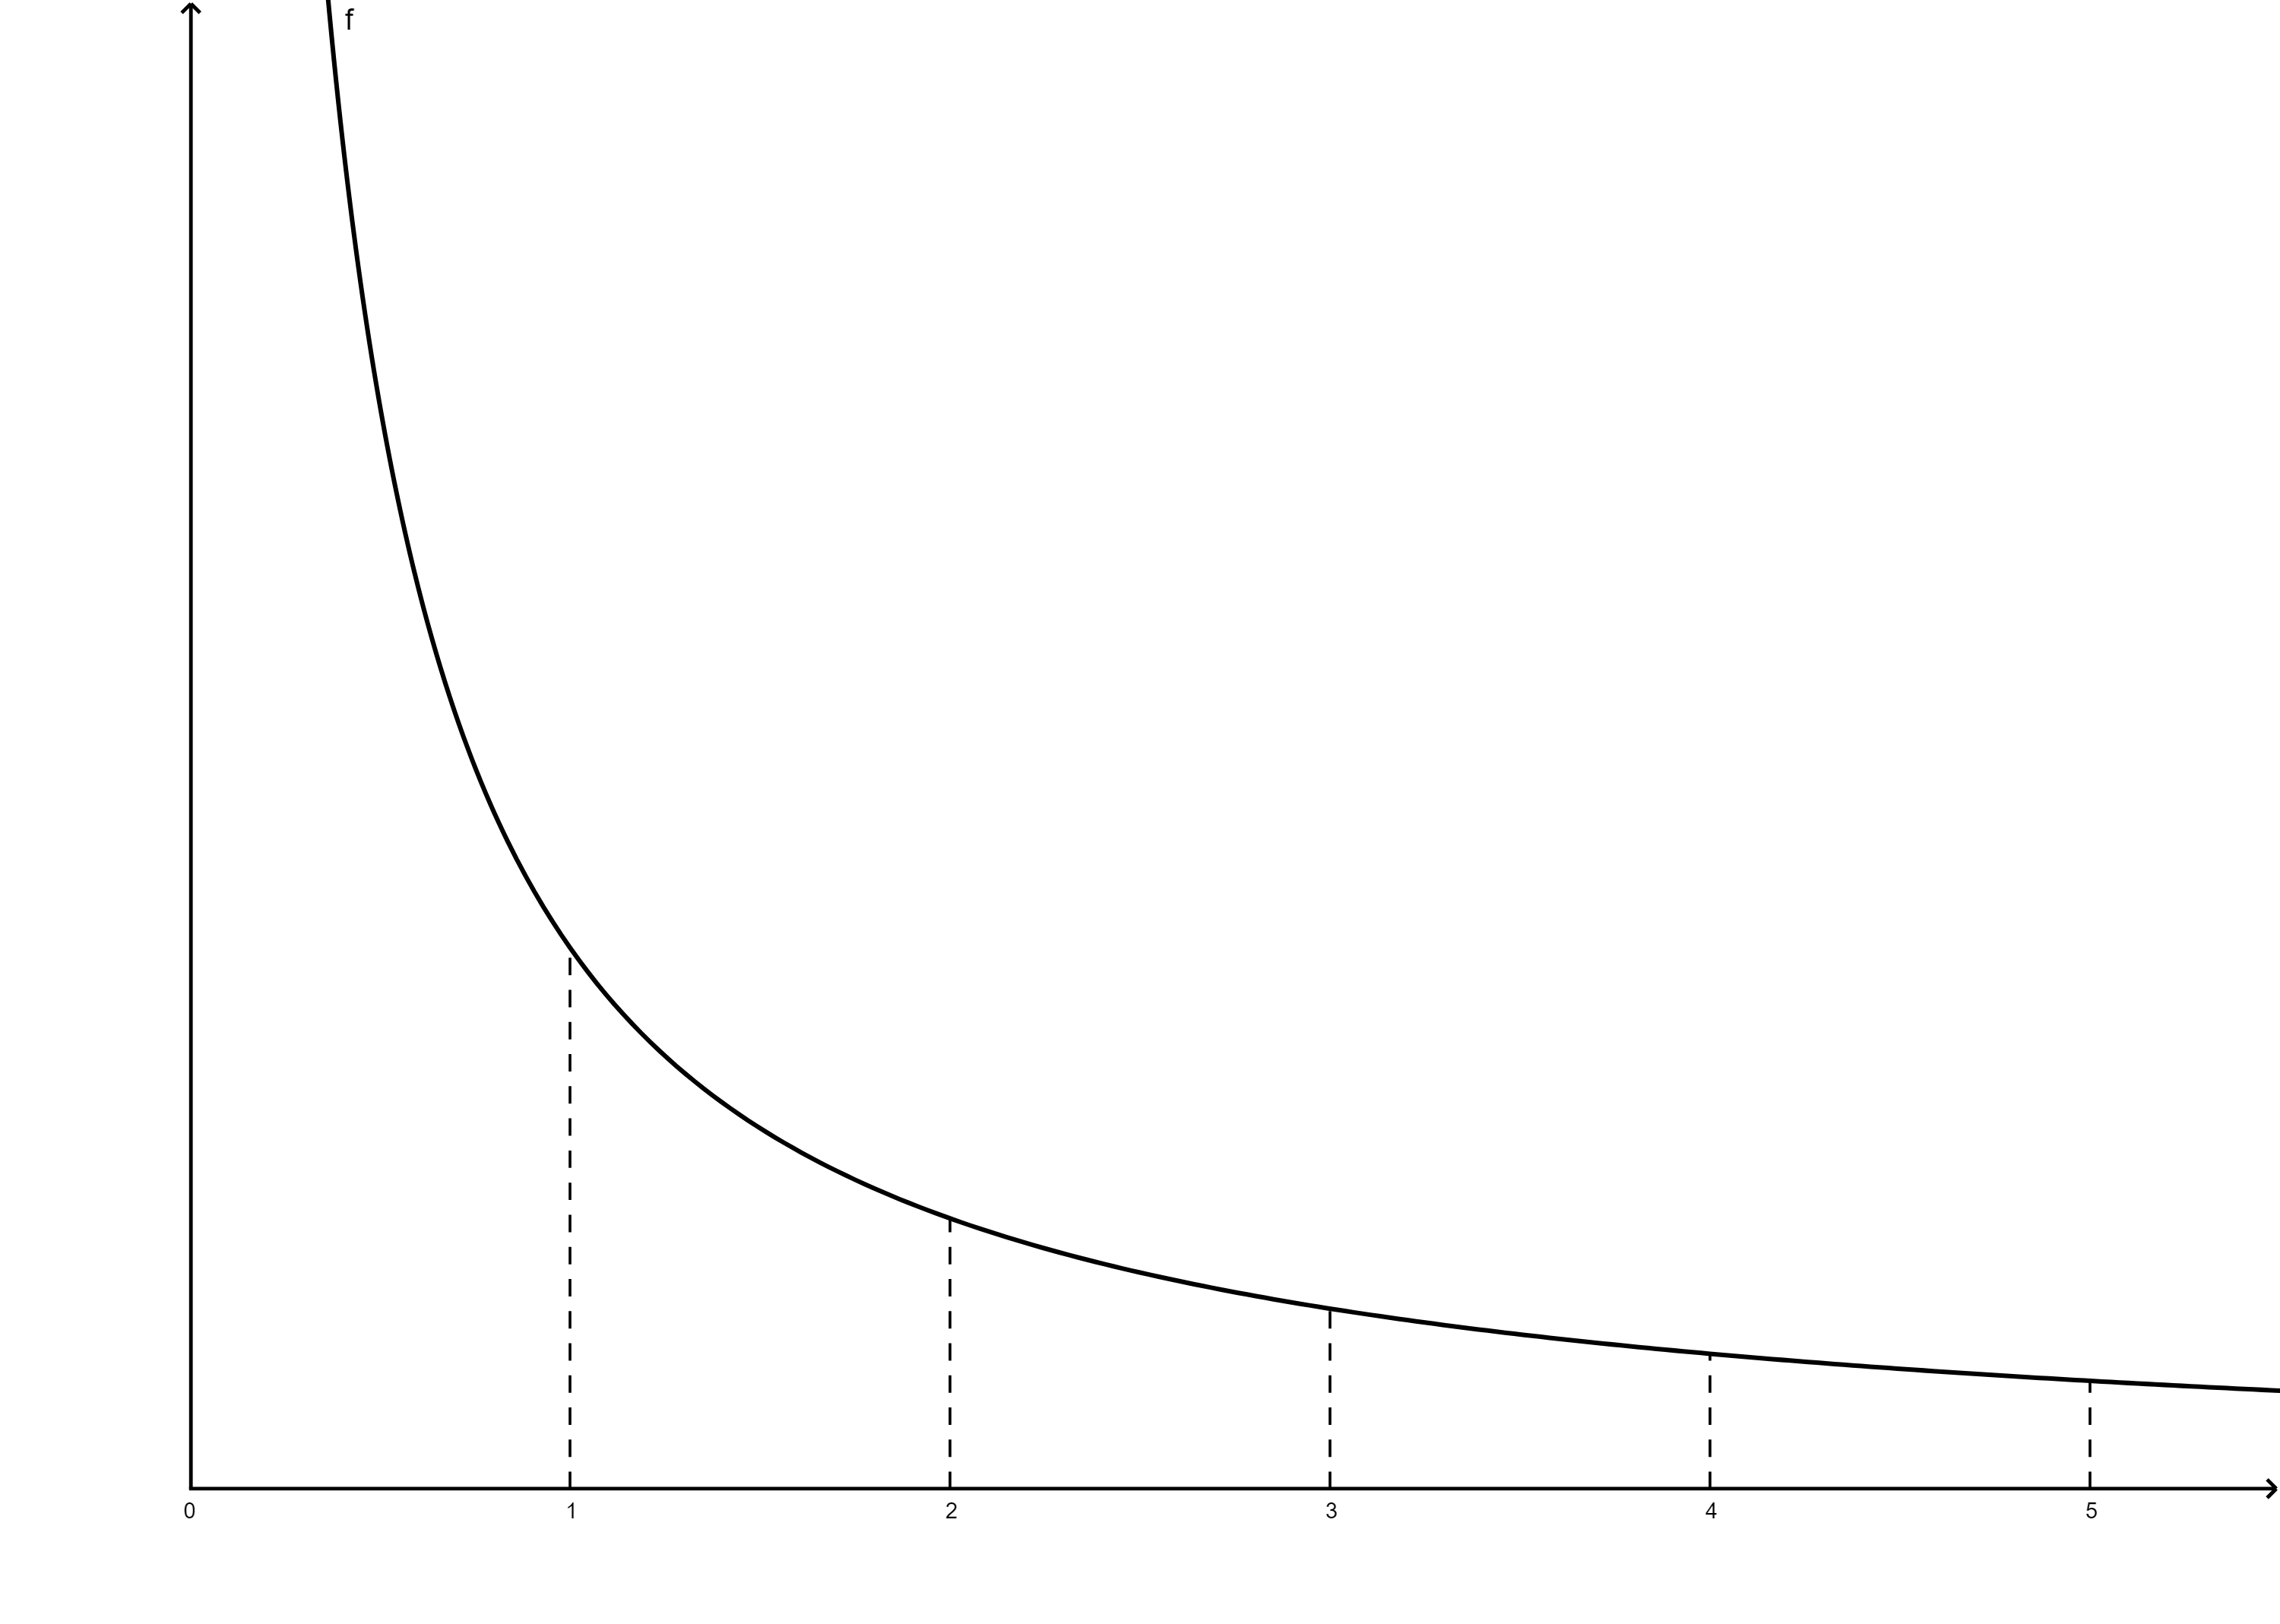
\includegraphics[width=0.5\linewidth]{3_2_1.png}\\
	$x \in [k; k+1], f(k+1) < f(x) < f(k) (k=1,2,\dots) \Rightarrow \\
	\Rightarrow f(k+1) \leq \int\limits_{k}^{k+1}f(x)\,dx \leq f(k) \Rightarrow \\
	\Rightarrow \sum\limits_{k=1}^{n}f(k+1) \leq \int\limits_{1}^{n+1}f(x)\,dx \leq \sum\limits_{k=1}^{n}f(k) = S_n, S_{n+1} - f(1) \leq \int\limits_{1}^{n+1}f(x)\,dx \leq S_n$\\
	$\Rightarrow$: \\
	$\baserow{f(n)}$ сходится $\Rightarrow$ [по теореме 1] $\Rightarrow S_n \leq S$\\
	$\forall t \in \bb{R} \; t > 1 \; \exists n \in \bb{N} t<n+1$ (аксиома Архимеда)\\
	$F(t) = \int\limits_{1}^{t}f(x)\,dx = \int\limits_{1}^{n+1}f(x)\,dx \leq S_n \ leq S$\\
	$F(t) \nearrow$ т.к. $F'=f(x) \Rightarrow \exists \lim\limits_{t \to +\infty} = F \leq S \Rightarrow \int\limits_{1}^{+\infty}f(x)\,dx$ сходится\\
	$\Leftarrow$:\\
	$\int\limits_{1}^{+\infty}f(x)\,dx = F$ сходится $\Rightarrow S_n \leq f(1) + \int\limits_{1}^{n+1}f(x)\,dx \leq f(1) + F \Rightarrow \\
	\Rightarrow [\text{по теореме 1}] \Rightarrow$ $\baserow{f(n)}$ сходится
\end{Proof}  %21  %Writing
    \section{Сходимость знакопеременных рядов}

\begin{Def}~\\
    Ряд $\sum_{n=1}^{+\infty}a_n$ называют знакопеременным, если существует бесконечно много $n \in \bb{N} a_n>0$
    и бесконечно много $k \in \mathbb{N} a_k<0$\\
\end{Def}

\begin{Def}~\\
    Ряд 
    \[
        \sum (-1)^{n-1} a_n = a_1 - a_2 + a_3 - a_4 + \dots
    \] 
    называют знакочередующимся, если $\forall n \in \mathbb{N} \quad a_n > 0 $
\end{Def}

\begin{Th}[признак Лейбница сходимость знакоперем. рядов]~\\
    Пусть ряд $\sum_{n=1}^{+\infty} (-1)^{n-1} a_n $ удовлетворяет следующим условиям:
    \begin{enumerate}
        \item $\forall n \in \mathbb{N}, \quad a_n > 0$
         
        \item $\{a_n\} \searrow$ строго, то есть $\forall n \in \bb{N}, \quad a_{n+1}<a_n$
        
        \item $\exists \lim\limits_{n \to \infty}=0$
        
    \end{enumerate}
    Тогда ряд $\sum_{n=1}^{+\infty} (-1)^{n-1} a_n = S$ сходится, $S$ - его сумма, при этом
    \begin{enumerate}
        \item $a_1-a_2<S<a_1$
        
        \item $\forall n \geqslant 1 \quad |S-S_n|<a_{n+1}$
    \end{enumerate}
\end{Th}

\begin{Proof}~\\
    Рассмотрим $\{S_{2n}\}$ тогда
    \[
        S_{2\,n}=\underbrace{(a_1-a_2)}_{>0}+\underbrace{(a_3-a_4)}_{>0}+\dots+\underbrace{(a_{2\,n-1}-a_{2\,n})}_{>0} 
    \]
    Также заметим
    \[
        S_{2\,(n+1)} - S_{2\,n}= a_{2\,n+1}-a_{2\,n+2} > 0 \quad \forall n \geqslant 1
    \]
    Так как по условию $\{a_n\}$ возрастает строго, тогда $S_{2n}<S_{2(n+1)}$ и $\{S_{2n}\}$ строго возрастает.\\
    Теперь рассмотрим другую группировку.
    \[
        S_{2n}=\underbrace{a_1}_{>0}-\underbrace{(a_2-a_3)}_{>0}-\dots-\underbrace{(a_{2n-2}-a_{2n-1})}_{>0}-\underbrace{a_{2n}}_{>0}
    \]
    Из этого следует 
    \[
        S_{2\,n}<a_1 \quad (n \geqslant 1) \qquad S_{2\,n}<a_1-a_2+a_3(n \geqslant 2)
    \]
    Значит $S_{2n}$ ограниченна сверху. Тогда
    \begin{gather*}
        \exists \lim\limits_{n \to \infty} S_{2\,n} = S = \sup\limits_{n\geqslant 1} S_{2\,n} \leqslant a_1-(a_2-a_3) < a_1
    \end{gather*}
    Значит
    \begin{gather*}
        \exists \lim\limits_{n \to \infty}S_{2\,n+1}= 
        \lim\limits_{n\to\infty}(\underbrace{S_{2\,n}}_{\to S}+\underbrace{a_{2n+1}}_{\to 0})=S\\
        \exists \lim\limits_{n \to \infty}S_{n}=S<a_1
    \end{gather*}
    Таким образом
    \[
        \sum_{n=2}^{+\infty} (-1)^{n-1} a_n=a_2-a_3+a_4-\dots=a_1-S<a_2
    \]
    Значит $a_1-a_2<S$ (пункт 1 доказан)\\
    Второй пункт доказывается аналогично\\
    \[
        (-1)^n\sum_{k=n+1}^{+\infty} (-1)^{k-1} a_k=a_{n+1}-a_{n+2} + \dots =\underbrace{(-1)^n(S-S_n)}_{0 < a_{n+1}-a_{n+2} < a_{n + 1}}
    \]
    Таким образом $|S-S_n| < a_{n+1}$
\end{Proof}

\textcolor{red}{не разобрано}
\begin{Example}~\\
    Доказ. $\sum_{n=1}^{+\infty} \frac{(-1)^{n-1}}{n}$ сходится(не абсолютно)\\
    $\frac{(-1)^{n-1}}{n}$ - ряд Лейбница\\
    Решение:\\
    $a_n=\frac{1}{n}>0, {a_n}\searrow$ строго, $a_n->0 (n->\infty)$ => по т.1 ряд Лейбница сходится\\
    Проверка на абс. сход.\\
    $\sum_{n=1}^{+\infty}| \frac{(-1)^{n-1}}{n}|=\sum_{n=1}^{+\infty}\frac{1}{n}$расход. (гарм. ряд)\\
\end{Example}

\textcolor{red}{не разобрано}
\begin{Example}~\\
	$\sum^{\infty}_{n=1} \frac{(-1)^{n-1}}{n^2}$ - сходится абсолютно\\
	$\sum^{\infty}_{n=1} \frac{(-1)^{n-1}}{ln(n+1)}$ - сходится (не абсолютно)\\
\end{Example}

\textcolor{red}{не разобрано}
\begin{Th}[Признак Дирихле]~\\
	Пусть $\sum^{infty}_{n=1}a_n\,b_n$ - числовой ряд, удовлетворяющий следующим условиям:
    \begin{enumerate}
        \item $\exists M > 0 : \forall n \in N |\sum^n_{k=1}a_k| \leq M$, то есть частичная сумма ряда ограничена
        
        \item $\{b_n\} \rightarrow 0$, то есть $\forall n \geq 1, b_k > 0;$ $\forall n \geq 1 b_{n+1} < b_n;$ $\exists lim b_n = 0$\\
        Тогда ряд $\sum^{infty}_{n=1}a_nb_n$ сходится и его сумма $|T| \leq Mb_1$
        
    \end{enumerate}
\end{Th}

\textcolor{red}{не разобрано}
\begin{Proof}~\\
	$T_n = a_1\,b_1 + \dots + a_n\,b_n = (a_1\,b_1) + (a_1\,b_2 + a_2\,b_2 - a_1\,b_2) + (a_1\,b_3 + a_2\,b_3 + a_3\,b_3 - a_1\,b_3 - a_2\,b_3) + \dots + a_1\,b_n + a_2\,b_n + \dots + a_n\,b_n - a_1\,b_n - a_2\,b_n - \dots - a_{n_1}\,b_n = $\\
	$ = S_1b_1 + S_2b_2 + \dots + S_nb_n - S_1b_2 - S_2b_3 - \dots - S_{n_1}b_n = S_1(b_1-b_2) + S_2(b_2 - b_3) + \dots + S_{n-1}(b_{n-1} - b_n) + S_nb_n$\\
	$\sum^{infty}_{k=1}a_kb_k = \sum^{\infty}_{k=1} S_k(b_k - b_{k+1})$\\
	$|S_k(b_k - b_{k+1})| < M(b_k - b_{k+1})$\\
	$\sum^{n}_{k=1}a_kb_k \leq \sum^{n}_{k=1} |S_k(b_k - b_{k+1})| < M\sum^{n}_{k=1}(b_k - b_{k+1}) = M(b_1 - b_n) \rightarrow Mb_1$\\
	По признаку сравнения ряд $\sum^{+\infty}_{n=1}S_k(b_k - b_{k+1}) = T$ - сходится\\
	$T_n = \sum^{n-1}_{k=1} S_k(b_k - b_{k+1}) + S_nb_n \rightarrow T \Rightarrow \exists limT_n = T$
\end{Proof}

\begin{Note}~\\
	Если
    \[
        \sum_{n=1}^{+\infty}(-1)^{n-1}b_n, \qquad b_n \rightarrow 0
    \]
    То значение суммы можно свести к следующему
	\[
        a_n = (-1)^{n-1}, |S_n| \leqslant 1    
    \]
\end{Note}

\textcolor{red}{Не разобран}
\begin{Example}~\\
	$\sum^{+\infty}_{n=1} \frac{cos n\alpha}{n^{\beta}}$\\
	$1) \alpha = 2\Pi k, k \in Z$ $cos(2 \Pi nk) = 1 \Rightarrow \sum^{\infty}_{n=1} \frac{1}{n^{\beta}}, \beta \leq 0 \Rightarrow \frac{1}{n^{\beta}}$ расходится, иначе сходится\\
	$2) \alpha \neq 2 \Pi k$\\
	$a_n = cos n\alpha, b_n = \frac{1}{n^{\beta}} \rightarrow 0$ при $\beta > 0$\\
	$S_n = cos \alpha + ... cos n\alpha$\\
	$2cos\alpha S_n = 2cos^2\alpha + 2cos\alpha cos2\alpha + ... + 2cos\alpha cosn\alpha = 1 + cos2\alpha + cos\alpha + cos3\alpha + ... + cos(n-1)\alpha + cos(n+1)\alpha = 1 + S_n - cosn\alpha + S_n - cos \alpha + cos(n+1)\alpha$\\
	$2(1-cos\alpha)S_n = 1 + cos n\alpha + cos\alpha - cos(n+1)\alpha$\\
	$2(1-cos\alpha)|S_n| = 4 \Rightarrow |S_n| \leq \frac{2}{1-cos\alpha} = M \Rightarrow$ ряд сходится\\
\end{Example}

  %20  %ReWriting
    %TODO Complete by images

\part{Функциональные последовательности и ряды}
\section{Равномерно сходящиеся функциональные последовательности}

\begin{Def}
	Пусть $\{f_n(x)\}$ это последовательность функций, определённых в некоторой области $D \subset \bb{R}$, тогда говорят, что эта последовательность поточечно сходится к $F(x), x \in D$\\
	$\text{т.е. } \exists \lim\limits_{n \to +\infty} = F(x), (x \in D) \Leftrightarrow \forall x \in D \; \exists \lim\limits_{n \to +\infty} = F(x)\\
	\text{т.е. } \forall \varepsilon > 0 \; \exists N \in \bb{N}, N=N(\varepsilon, x) \; \forall n > N \; |f_n(x) - F(x)| < \varepsilon$
\end{Def}

\begin{Example}
	Let there be images\\
	$f_n(x) = x^n, x \in [0;1]$\\
	$\lim\limits_{n \to +\infty}x^n = F(x) \Rightarrow F(x) = 
	\begin{cases}
	0, x \in [0;1)\\
	1, x=1
	\end{cases}$
\end{Example}

\begin{Def}
	Пусть $\{f_n(x)\}$ это последовательность функций, определённых в некоторой области $D \subset \bb{R}$, тогда говорят, что эта последовательность равномерно сходится к $F(x), x \in D \Leftrightarrow \\
	\Leftrightarrow \forall \varepsilon > 0 \; \exists N \in \bb{N}, N=N(\varepsilon, x) \; \forall n > N \; \forall x \in D \; |f_n(x) - F(x)| < \varepsilon$
	Отличие от поточечной сходимости получается только в том, что номер, с которого начинается пренебрежимо малое отставание от F не зависит от x\\
	Обозначают: $f_n(x) \rightrightarrows F(x) (n \to +\infty; x \in D)$
\end{Def}

\begin{Note}[Геометрический смысл равномерной сходимости]
	Let there be image
\end{Note}

\begin{Note}
	Let there be image\\
	$f_n(x) = x^n; x \in [0;1] \: \: f_n(x) \underset{n \to +\infty}{\rightarrow}F(x) \\
	f_n(x) \cancel{\rightrightarrows} F(x)$, где $F(x) = 
	\begin{cases}
	0, x \in [0;1)\\
	1, x = 1
	\end{cases} 0 < \varepsilon < \frac{1}{2}$
\end{Note}

\begin{Th}[Критерий Коши равномерной сходимости функциональных последовательностей]
	Пусть $\{f_n(x)\}$ - функциональная последовательность, где $x \in D$. Тогда $\{f_n(x)\}$ равномерно стремится к $F(x)$ при $n \to +\infty; x \in D \Leftrightarrow \\
	\Leftrightarrow \forall \varepsilon > 0 \; \exists N(\varepsilon) \in \bb{N} \; \forall n,m \geq N \; \forall x \in D \; |f_n(x)-f_m(x)| < \varepsilon$
\end{Th}

\begin{Proof}
	$\; \\ \Rightarrow \\$
	Пусть $f_n(x)$ равномерно сходится к $F(x)$ для $n \to +\infty, x \in D \Rightarrow \\$
	$\Rightarrow \forall n \geq N \; \forall x \in D \; |f_n(x) - F(x)| < \frac{\varepsilon}{2};\\$
	$\Rightarrow \forall m \geq N \; \forall x \in D \; |f_m(x) - F(x)| < \frac{\varepsilon}{2}\\
	|f_n(x) - f_m(x)| = |f_n(x) - F(x) + F(x) - f_m(x)| \leq |f_n(x) - F(x)| +\\
	+ |f_m(x) - F(x)| < \frac{\varepsilon}{2} + \frac{\varepsilon}{2} = \varepsilon \Rightarrow |f_n(x) - f_m(x)| < \varepsilon\\$
	$\; \\ \Leftarrow \\$
	$\forall \varepsilon \; \exists N(\varepsilon) \; \forall n,m \geq N \: |f_n(x) - f_m(x)| < \frac{\varepsilon}{2} \Rightarrow \\
	\text{Тогда} \; \forall x \in D \; f_m(x) \underset{n \to +\infty}{\rightarrow} F(x) $ (по критерию Коши для числовой последовательности)\\
	$\Rightarrow (m \to +\infty) \Rightarrow |f_n(x) - F(x)| \leq \frac{\varepsilon}{2} < \varepsilon \Rightarrow f_n(x) \rightrightarrows F(x) (n \to +\infty; x \in D)$
\end{Proof}

\begin{Th}[О непрерывности предела равномерно сходящихся функциональных последовательностей]
	Пусть $\forall n \geq 1 \text{ функции } f_n(x) \in C_{[a;b]}$.\\
	Тогда $f_n(x) \rightrightarrows F(x) (n \to +\infty, x \in [a;b]) \Rightarrow F(x) \in C_{[a;b]}$ 
\end{Th}

\begin{Proof}
	Надо доказать, что
	1. $\forall x_0 \in [a;b] \; \exists \lim\limits_{x \to x_0}F(x) = F(x_0) \text{и} 
	\begin{cases}
	\exists F(a+0) = F(a)\\
	\exists F(b-0) = F(b)
	\end{cases}\\$
	Пусть $x_0 \in [a;b], f_n(x) \in C_{[a;b]} \Rightarrow \text{[по теореме Кантора]} \Rightarrow \\
	\Rightarrow f_n(x) \text{равномерно непрерывна на} [a;b] \forall n in \bb{N},$\\
	т.е. $\forall \varepsilon > 0 \; \exists \delta > 0, \delta = \delta(\varepsilon, n) \; \forall x, x_0 \in [a;b] \; |x-x_0| < \delta \: |f_n(x)-f_n(x_0)| < \frac{\varepsilon}{3}$\\
	$f_n(x) \rightrightarrows F(x) (n \to +\infty; x \in D) \text{ для } \varepsilon > 0 \\
	\exists N \in \bb{N} \; \forall n \geq N \; \forall x, x_0 \in [a;b] |f_n(x) - F(x)| < \frac{\varepsilon}{3}, |f_n(x_0) - F(x_0)| < \frac{\varepsilon}{3}$\\
	Для $n = N: |f_N(x) - F(x)| < \frac{\varepsilon}{3}; |f_N(x_0) - F(x_0)| < \frac{\varepsilon}{3} \Rightarrow\\
	\Rightarrow |F(x) - F(x_0)| = |F(x) - f_N(x) + f_N(x) - F(x_0) - f_N(x_0) + f_N(x_0)| \leq \\
	\leq |f_N(x) - F(x)| + |f_N(x_0) - F(x_0)| + |f_N(x) - f_N(x_0)| < \frac{\varepsilon}{3} + \frac{\varepsilon}{3} + \frac{\varepsilon}{3} = \varepsilon$
	$\delta = \delta(\varepsilon, n)$, т.е. $\delta$ не зависит от $x$\\
	$\forall \varepsilon > 0 \; \exists N \in \bb{N} \; \exists \delta(\varepsilon, n) > 0 \; \forall x, x_0 \in [a;b] \; |x-x_0| < \delta \Rightarrow |F(x) - F(x_0)| < \varepsilon\\
	\Rightarrow F(x) \text{непрерывна на } [a;b]$
\end{Proof}

\begin{Note}
	$\lim\limits_{x \to x_0}(\lim\limits_{n \to +\infty}(f_n(x))) = \lim\limits_{n \to +\infty}(\lim\limits_{x \to x_0}(f_n(x))) \Leftrightarrow F(x) \in C_{[a;b]}, x,x_0 \in [a;b]$
\end{Note}

\begin{Th}[Об интегрировании равномерно сходящихся функциональных последовательностей]
	Пусть функции $f_n(x) \in C_[a;b]$ и $f_n(x) \rightrightarrows F(x), (n \to +\infty, x \in [a;b]) \Rightarrow\\
	\Rightarrow \exists \lim\limits_{n \to +\infty}\int\limits_{a}^{b}f_n(x)dx = \int\limits_{a}^{b}F(x)dx$
\end{Th}

\begin{Proof}
	$\; \\
	f_n(x) \rightrightarrows F(x) (n \to +\infty; x \in [a;b]) \Rightarrow\\
	\Rightarrow \forall \varepsilon > 0 \; \exists N(\varepsilon) \in \bb{N} \; \forall n \geq N \; \forall x \in [a;b] |f_n(x) - F(x)| < \frac{\varepsilon}{b - a}\\
	|\int\limits_{a}^{b}f_n(x)dx - \int\limits_{a}^{b}F(x)dx| = |\int\limits_{a}^{b}f_n(x)dx - F(x)dx| \leq \\
	\leq |\int\limits_{a}^{b}f_n(x)dx - F(x)dx| \leq \frac{\varepsilon}{b - a}(b-a) =  \varepsilon \Rightarrow\\
	\Rightarrow \forall \varepsilon > 0 \; \exists N(\varepsilon) \in \bb{N} \; \forall n \geq N \; \forall x \in [a;b] |\int\limits_{a}^{b}f_n(x)dx - \int\limits_{a}^{b}F(x)dx| \leq \varepsilon \Rightarrow\\
	\Rightarrow \exists \lim\limits_{n \to +\infty}\int\limits_{a}^{b}f_n(x)dx = \int\limits_{a}^{b}F(x)dx$
\end{Proof}

\begin{Note}
	$\lim\limits_{n \to +\infty}\int\limits_{a}^{b}f_n(x)dx = \int\limits_{a}^{b} \lim\limits_{n \to +\infty}f_n(x)dx$
\end{Note}

\begin{Note}
	Теорема 3 неверна в случае поточечной, а не равномерной, сходимости.\\
	Let there be images\\
	$f_n(x) \in C_{[0;1]}. f_n(x) \rightarrow 0 (n \to +\infty; x \in [0;1])\\
	\int\limits_{0}^{1}f_n(x) = \text{[как площадь треугольника]} = \frac{2}{n} \frac{n}{2} = 1 \rightarrow 1 (n \to +\infty)$\\
	Но при этом $\int\limits_{0}^{1}F(x) = 0 \rightarrow 0 (n \to +\infty) \Rightarrow\\
	\Rightarrow \lim\limits_{n \to +\infty}\int\limits_{a}^{b}f_n(x)dx \neq \int\limits_{a}^{b}F(x)dx$
\end{Note}

\begin{Th}[О дифференциировании равномерно сходящихся функциональных рядов]
	Пусть $f_n(x) \in C_{[a;b]}^{1}, \text{т.е.} \exists f_n'(x) \in C_{[a;b]}$ и выполнены условия:\\
	\begin{enumerate}
		\item $f_n'(x) \rightrightarrows \varphi (x) (n \to +\infty; x \in [a;b])$
		\item $\exists x_0 \in [a;b] \; f_n(x_0) \rightarrow A (n \to +\infty)$
	\end{enumerate}
	Тогда:
	\begin{enumerate}
		\item $\exists F(x) \in C_{[a;b]}^{1} \; f_n(x) \rightrightarrows F(x) (n \to +\infty; x \in [a;b])$
		\item $F'(x) = \varphi'(x) (x \in [a;b])$
	\end{enumerate}
\end{Th}

\begin{Proof}
	$F(x) = A + \int\limits_{x_0}^{x}\varphi(t)dt$\\
	$\begin{cases}
	f_n'(x) \in C_{[a;b]}\\
	f_n'(x) \rightrightarrows \varphi(x)
	\end{cases} \Rightarrow \text{[по теореме 2]} \Rightarrow \varphi(t) \in C_{[a;b]} \Rightarrow\\
	\Rightarrow \varphi(t)$ интегрируема $\Rightarrow \text{[по теореме Барроу]} \Rightarrow \exists F'(x) = \varphi(x) (x \in [a;b])$\\
	$|f_n(x) - F(x)| = |\int\limits_{x_0}^{x}f_n'(t)dt + f_n(x_0) - A - \int\limits_{x_0}^{x}\varphi(t)dt| = \\
	= |\int\limits_{x_0}^{x}(f_n'(t) - \varphi(t))dt + f_n(x_0) - A| \leq |\int\limits_{x_0}^{x}|(f_n'(t) - \varphi(t))|dt| + |f_n(x_0) - A|$\\
	$\forall \varepsilon > 0 \; \exists N_1(\varepsilon) \in \bb{N} \; \forall n \geq N_1 \; \forall t \in [a;b] |f_n'(x) - \varphi(t)| < \frac{\varepsilon}{2(b-a)}$ т.к. $f_n(t)$ сходится к $\varphi(t)$\\
	Для $\varepsilon > 0 \exists N \geq N_1 \; \forall n \geq N \: |f_n(x_0) - A| < \frac{\varepsilon}{2}$\\
	Итого:\\
	$\forall \varepsilon > 0 \; \exists N(\varepsilon) \in \bb{N} \; \forall n \geq N \: |\int\limits_{x_0}^{x}|(f_n'(t) - \varphi(t))|dt| < \frac{\varepsilon}{2(b-a)}|\int\limits_{x_0}^{x}dt| = \\
	= \frac{\varepsilon |x-x_0|}{2(b-a)} \leq \frac{\varepsilon(b-a)}{2(b-a)} = \frac{\varepsilon}{2}$\\
	Прибавим к этому, что $|f_n(x_0) - A| < \frac{\varepsilon}{2}$ и получим:\\
	$|f_n(x) - F(x)| < \frac{\varepsilon}{2} + \frac{\varepsilon}{2} = \varepsilon$\\
	Итого:\\
	$\forall x \in [a;b] |f_n(x) - F(x)| < \varepsilon\\
	\forall \varepsilon > 0 \; \exists N(\varepsilon) \; \forall n \geq N \; \forall x \in [a;b] \: |f_n(x) - F(x)| < \varepsilon \Rightarrow f_n(x) \rightrightarrows F(x), (n \to +\infty, x \in [a;b])$ 1я часть доказана %Тут есть доказательство второй части, которое я пропустил или какой-то подвох?
\end{Proof}
  %21  %Writing
    
    %\begin{figure}[bh]
    %    \noindent\centering{
    %        \includegraphics[width=75mm]{1_1_1.png}
    %        \caption{}
    %    }
    %\end{figure}
    
\end{document}